% This LaTeX document needs to be compiled with XeLaTeX.
\documentclass[10pt]{article}
\usepackage[utf8]{inputenc}
\usepackage{ucharclasses}
\usepackage{graphicx}
\usepackage[export]{adjustbox}
\graphicspath{ {./images/} }
\usepackage{caption}
\usepackage{amsmath}
\usepackage{amsfonts}
\usepackage{amssymb}
\usepackage[version=4]{mhchem}
\usepackage{stmaryrd}
\usepackage{multirow}
\usepackage{polyglossia}
\usepackage{fontspec}
\setmainlanguage{vietnamese}
\setotherlanguages{english, hindi}
\newfontfamily\vietnamesefont{CMU Serif}
\IfFontExistsTF{Noto Serif Devanagari}
{\newfontfamily\hindifont{Noto Serif Devanagari}}
{\IfFontExistsTF{Kohinoor Devanagari}
  {\newfontfamily\hindifont{Kohinoor Devanagari}}
  {\IfFontExistsTF{Devanagari MT}
    {\newfontfamily\hindifont{Devanagari MT}}
    {\IfFontExistsTF{Lohit Devanagari}
      {\newfontfamily\hindifont{Lohit Devanagari}}
      {\IfFontExistsTF{FreeSerif}
        {\newfontfamily\hindifont{FreeSerif}}
        {\newfontfamily\hindifont{Arial Unicode MS}}
}}}}
\IfFontExistsTF{CMU Serif}
{\newfontfamily\lgcfont{CMU Serif}}
{\IfFontExistsTF{DejaVu Sans}
  {\newfontfamily\lgcfont{DejaVu Sans}}
  {\newfontfamily\lgcfont{Georgia}}
}
\setDefaultTransitions{\lgcfont}{}
\setTransitionsFor{Vietnamese}{\vietnamesefont}{\lgcfont}
\setTransitionsForDevanagari{\hindifont}{\rmfamily}

%New command to display footnote whose markers will always be hidden
\let\svthefootnote\thefootnote
\newcommand\blfootnotetext[1]{%
  \let\thefootnote\relax\footnote{#1}%
  \addtocounter{footnote}{-1}%
  \let\thefootnote\svthefootnote%
}

%Overriding the \footnotetext command to hide the marker if its value is `0`
\let\svfootnotetext\footnotetext
\renewcommand\footnotetext[2][?]{%
  \if\relax#1\relax%
    \ifnum\value{footnote}=0\blfootnotetext{#2}\else\svfootnotetext{#2}\fi%
  \else%
    \if?#1\ifnum\value{footnote}=0\blfootnotetext{#2}\else\svfootnotetext{#2}\fi%
    \else\svfootnotetext[#1]{#2}\fi%
  \fi
}

\begin{document}
\captionsetup{singlelinecheck=false}
\section*{HUÚNG DÂN GHÁT}
\section*{Churong 1. ESHER - HIPID. XA PHONG VA CHÁT GHET RÚA}
\begin{center}
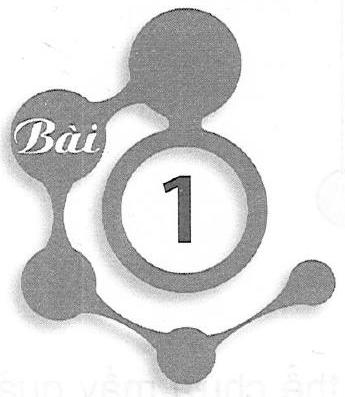
\includegraphics[max width=\textwidth]{2025_10_23_b4e16b74380d0f7e7700g-001}
\end{center}

\section*{ESTER - LIPID}
1.1. Đáp án C.\\
1.2. Đáp án B. Gồm 1 carboxylic acid và 2 ester.\\
1.3. Đáp án A. Độ tan trong nước của ester giảm khi độ dài mạch carbon tăng.\\
1.4. Đáp án C. Ester có nhiệt độ sôi thấp hơn alcohol và carboxylic acid có cùng số nguyên tử carbon hoặc có phân tử khối tương đương.\\
1.5. Đáp án A.\\
1.6. Đáp án C .\\
1.7. Đáp án C.\\
1.8. Đáp án C. Các phát biểu đúng là a ), b) và d).

Chú ý:

\begin{itemize}
  \item Dù diethyl ether có nhiệt độ sôi thấp hơn nhiều so với ethyl acetate nhưng không thể thu ethyl acetate sau khi chiết bằng cách dùng đèn cồn đun nhẹ cho dung môi diethyl ether bay hơi, do hơi diethyl ether đặc biệt dễ cháy, khi gặp ngọn lửa đèn cồn sẽ gây hoả hoạn, nguy hiểm.
  \item Cũng không nên sử dụng đèn cồn trong phương pháp chưng cất đơn giản để tách ethyl acetate ra khỏi dung môi diethyl ether sau khi chiết do diethyl ether có thể rò rỉ gây hoả hoạn. Có thể dùng bếp điện để đun cách thuỷ, nhưng an toàn nhất vẫn là dùng nước nóng tưới liên tục lên bình cầu chưng cất.
\end{itemize}

\begin{table}[h]
\begin{center}
\captionsetup{labelformat=empty}
\caption{1.9.}
\begin{tabular}{|l|l|l|l|l|}
\hline
Tên gọi & Công thức cấu tạo & Phân loại & Phân tử khối & Nhiệt độ sôi $\left({ }^{\circ} \mathrm{C}\right)$ \\
\hline
diethyl ether & $\mathrm{C}_{2} \mathrm{H}_{5} \mathrm{OC}_{2} \mathrm{H}_{5}$ & ether & 74 & 34 \\
\hline
ethyl formate & $\mathrm{HCOOC}_{2} \mathrm{H}_{5}$ & ester & 74 & 54 \\
\hline
methyl acetate & $\mathrm{CH}_{3} \mathrm{COOCH}_{3}$ & ester & 74 & 57 \\
\hline
butanal & $\mathrm{CH}_{3} \mathrm{CH}_{2} \mathrm{CH}_{2} \mathrm{CHO}$ & aldehyde & 72 & 76 \\
\hline
butan-1-ol & $\mathrm{CH}_{3} \mathrm{CH}_{2} \mathrm{CH}_{2} \mathrm{CH}_{2} \mathrm{OH}$ & alcohol & 74 & 118 \\
\hline
propanoic acid & $\mathrm{CH}_{3} \mathrm{CH}_{2} \mathrm{COOH}$ & carboxylic acid & 74 & 141 \\
\hline
\end{tabular}
\end{center}
\end{table}

1.10. Nhiệt độ sôi của carboxylic acid và alcohol cao hơn so với các chất có phân tử khối xấp xỉ hoặc tương đương còn lại trong bảng, trong đó nhiệt độ sôi của carboxylic acid cao hơn alcohol. Đó là do chỉ có carboxylic acid và alcohol tạo được liên kết hydrogen liên phân tử, trong đó liên kết hydrogen giữa các phân tử carboxylic acid bền hơn so với giữa các phân tử alcohol.

\begin{table}[h]
\begin{center}
\captionsetup{labelformat=empty}
\caption{1.11.}
\begin{tabular}{|c|c|c|}
\hline
Ester & \begin{tabular}{c}
Acid tạo thành và \\
tên gọi \\
\end{tabular} & \begin{tabular}{c}
Alcohol tạo thành và \\
tên gọi \\
\end{tabular} \\
\hline
$\mathrm{C}_{2} \mathrm{H}_{5} \mathrm{COOCH}_{3}$ & \begin{tabular}{c}
$\mathrm{C}_{2} \mathrm{H}_{5} \mathrm{COOH}$ \\
(propionic acid) \\
\end{tabular} & \begin{tabular}{c}
$\mathrm{CH}_{3} \mathrm{OH}$ \\
(methanol) \\
\end{tabular} \\
\hline
\end{tabular}
\end{center}
\end{table}

\begin{center}
\begin{tabular}{|l|l|l|}
\hline
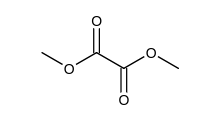
\includegraphics{smile-d54167939222949db4b67932cda17e447bc68f7c} & \begin{tabular}{l}
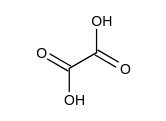
\includegraphics{smile-b4c509572bfd6d29fae388032ddf8a35b1df7ddd} \\
(oxalic acid) \\
\end{tabular} & $\mathrm{CH}_{3} \mathrm{OH}$ (methanol) $\mathrm{C}_{2} \mathrm{H}_{5} \mathrm{OH}$ (ethanol) \\
\hline
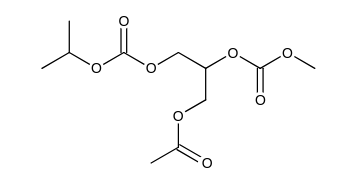
\includegraphics{smile-970dc952bae2e954252dfbf5237bfc9073dd673f} & HCOOH (formic acid) $\mathrm{CH}_{3} \mathrm{COOH}$ (acetic acid) & \begin{tabular}{l}
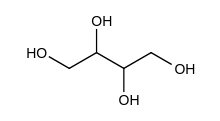
\includegraphics{smile-a01d03643f56ddc1cd55b7a5f16df71719337409} \\
(glycerol) \\
\end{tabular} \\
\hline
\end{tabular}
\end{center}

1.12. Do ester không tạo được liên kết hydrogen giữa các phân tử nên ester có nhiệt độ sôi thấp hơn so với các alcohol và carboxylic acid có cùng số nguyên tử carbon. Mặt khác, nhiệt độ sôi của carboxylic acid luôn cao hơn alcohol có cùng số nguyên tử carbon hoặc có phân tử khối tương đương, còn nhiệt độ sôi của các chất cùng dãy đồng đẳng tăng khi số nguyên tử carbon tăng, ta có kết quả sau:

\begin{center}
\begin{tabular}{|l|c|l|c|}
\hline
\multicolumn{1}{|c|}{Họp chất} & \multicolumn{1}{|c|}{\begin{tabular}{c}
Nhiệt độ \\
sôi $\left({ }^{\circ} \mathrm{C}\right)$ \\
\end{tabular}} & \multicolumn{1}{|c|}{Hợp chất} & \begin{tabular}{c}
Nhiệt độ \\
sôi ( ${ }^{\circ} \mathrm{C}$ ) \\
\end{tabular} \\
\hline
HCOOH & 100,8 & $\mathrm{CH}_{3} \mathrm{CH}_{2} \mathrm{CH}_{2} \mathrm{COOH}$ & 164 \\
\hline
$\mathrm{CH}_{3} \mathrm{CH}_{2} \mathrm{CH}_{2} \mathrm{CH}_{2} \mathrm{OH}$ & 117,7 & $\mathrm{CH}_{3} \mathrm{CH}_{2} \mathrm{CH}_{2} \mathrm{CH}_{2} \mathrm{CH}_{2} \mathrm{OH}$ & 138 \\
\hline
$\mathrm{HCOOCH}_{2} \mathrm{CH}_{2} \mathrm{CH}_{2} \mathrm{CH}_{3}$ & 107 & $\mathrm{CH}_{3} \mathrm{COOCH}_{2} \mathrm{CH}_{3}$ & 77 \\
\hline
\end{tabular}
\end{center}

1.13. $X$ có thể có 3 công thức cấu tạo sau:\\
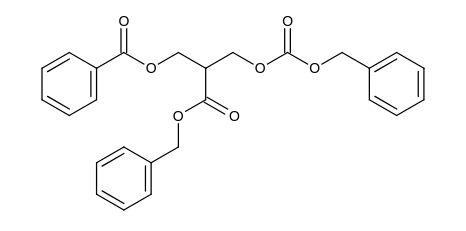
\includegraphics{smile-d6348fae1e8764fdcbca8c349238f4da9aad0aef}\\
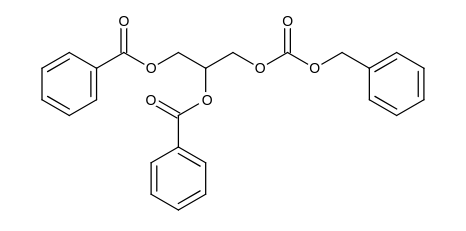
\includegraphics{smile-af940decc1528d6904d789773681f5c04f7fb945}\\
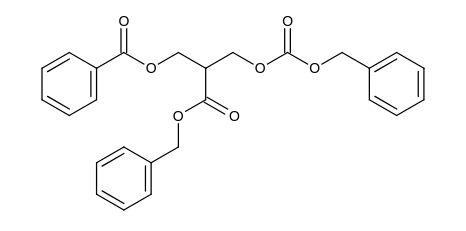
\includegraphics{smile-2bfd6534941131a22f97a9093713d785a938f66b}\\
1.14. Ester có mùi thơm được nhận biết thông qua khứu giác. Điều này phụ thuộc vào hiện tượng bay hơi của ester, có nghĩa liên quan đến nhiệt độ sôi của ester. Các ester có phân tử khối lớn hơn không có mùi thơm mạnh do có nhiệt độ sôi cao hơn các ester có phân tử khối nhỏ. Ngoài\\
ra, các ester có phân tử khối lớn tuy hoà tan được trong chất béo nhưng không hoà tan được trong nước, vì vậy ngay cả khi chúng đến được mũi, chúng cũng sẽ không đi qua lớp chất nhầy để đến được các cơ quan thụ cảm mùi hương. Mặt khác với kích thước cồng kềnh, ester có phân tử khối lớn không tương thích với các thụ thể mùi hương. Do đó, ester có phân tử khối lớn hơn thì mùi thơm nhẹ hơn.\\
1.15. Mặc dù hương vị và mùi "trái cây" của ester rất dễ chịu, nhưng chúng hiếm khi được sử dụng trong các loại nước hoa cao cấp. Lí do là các ester không bền với mồ hôi. Khi tiếp xúc với mồ hôi, chúng bị thuỷ phân tạo ra các carboxylic acid thường có mùi không dễ chịu như các ester. Ví dụ, butyric acid có mùi giống như bơ bị ôi thiu, đây cũng là chất có trong thành phần các chất tạo nên mùi hôi cơ thể, được tạo thành do sự thuỷ phân ethyl butyrate và methyl butyrate. Ethyl butyrate và methyl butyrate là những ester có mùi hấp dẫn của dâu và táo.

Trong nước hoa cao cấp, chất tạo hương có thể là hydrocarbon (terpene), aldehyde hoặc ketone. Ví dụ với terpene, myrcene $\left(\mathrm{C}_{10} \mathrm{H}_{16}\right)$ được tìm thấy trong nhiều cây gai dầu, trái cây họ cam quýt, xoài, nguyệt quế, đinh hương, ... Limonene, đồng phân của myrcene được tìm thấy trong vỏ của các loại trái cây có múi, rau mùi, cần tây và hạt hồi, ... Với aldehyde, hầu như không loại nước hoa nào trên thế giới tồn tại mà không có sự hiện diện của chúng, chẳng hạn decanal ( $\mathrm{C}_{10} \mathrm{H}_{20} \mathrm{O}$ ), undecanal ( $\mathrm{C}_{11} \mathrm{H}_{22} \mathrm{O}$ ), có trong thành phần tinh dầu cam, quýt, hoa hồng, $\ldots$ đã góp phần cùng một số chất tạo mùi khác tạo nên hương thơm đặc sắc của những loại nước hoa nổi tiếng nhất thế giới.

Muscone ( $\mathrm{C}_{16} \mathrm{H}_{30} \mathrm{O}$ ) là một ketone chủ yếu tạo nên mùi thơm của xạ hương. Xạ hương tạo cho nước hoa một mùi thơm đặc biệt dễ chịu và bền lâu. Ngày nay, xạ hương được sử dụng trong nước hoa đều là xạ hương tổng hợp.\\
1.16. Chất béo là những chất có phân tử lớn, cồng kềnh hơn nhiều so với phân tử nước. Do đó trong cùng một thể tích không gian, số các phân tử nước hiện diện nhiều hơn so với số các phân tử chất béo. Vì thế, chất béo có khối lượng riêng nhỏ hơn nước nên chất béo nhẹ hơn nước.

Chất béo là phân tử không phân cực nên không tan trong dung môi phân cực là nước.\\
1.17. Trong công nghiệp thực phẩm, dầu thực vật được chuyển đổi từ chất lỏng sang chất rắn bằng phản ứng hydrogen hoá. Bơ thực vật (margarine) được "làm cứng" theo cách này để chúng trở nên rắn hoặc bán rắn trong điều kiện thường. Việc làm này sẽ giúp kéo dài thời hạn sử dụng của thực phẩm và giữ hương vị ổn định do khó bị oxi hoá hơn dầu thực vật.\\
1.18. a) Vì tỉ lệ mol giữa pentyl alcohol và acetic acid là $1: 1$ nên

$$
\begin{gathered}
\frac{22 \times 0,81}{88}=\frac{V \times 1,05}{60} \\
\Rightarrow V=11,57(\mathrm{~mL})
\end{gathered}
$$

b) Đá bọt là loại đá được hình thành bởi dung nham núi lửa phun trào, có độ xốp cao và nhẹ.

Vai trò của đá bọt là giúp hỗn hợp phản ứng không bị sôi mạnh.\\
c) Phản ứng xảy ra trong thí nghiệm là phản ứng ester hoá. Đây là phản ứng thuận nghịch:\\
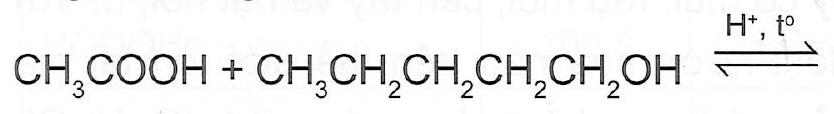
\includegraphics[max width=\textwidth, center]{2025_10_23_b4e16b74380d0f7e7700g-005}

$$
\mathrm{CH}_{3} \mathrm{COOCH}_{2} \mathrm{CH}_{2} \mathrm{CH}_{2} \mathrm{CH}_{2} \mathrm{CH}_{3}+\mathrm{H}_{2} \mathrm{O}
$$

d) Trên lí thuyết, $n_{\text {ester }}=n_{\text {carboxylic acid }}=n_{\text {alcohol }}=0,2025 \mathrm{~mol}$.

Vậy hiệu suất ester hoá là:

$$
H=\frac{17}{0,2025 \times 130} \times 100 \%=64,58 \%
$$

e) Hạt silica gel có nhiệm vụ hấp thụ nước sinh ra trong phản ứng ester hoá, nhờ đó giúp hiệu suất ester hoá tăng lên.

Hạt silica gel có màu xanh do được nhuộm $\mathrm{CoCl}_{2}$. Khi hấp thụ một lượng nước bão hoà sẽ chuyển sang màu hồng, là màu của phức chất $\left[\mathrm{Co}\left(\mathrm{H}_{2} \mathrm{O}\right)_{6}\right] \mathrm{Cl}_{2}$, hay viết dưới dạng muối ngậm nước là $\mathrm{CoCl}_{2} \cdot 6 \mathrm{H}_{2} \mathrm{O}$.

Bằng cách sấy khô silica gel đã hấp thụ nước, ta có thể tái sử dụng các hạt silica gel đã bão hoà nước.\\
1.19. Một lượng nhỏ chất béo là phần thiết yếu của chế độ ăn uống cân bằng, lành mạnh. Chất béo là nguồn cung cấp các acid béo thiết yếu mà cơ thể không tự tổng hợp được. Ngoài ra, chất béo còn giúp cơ thể hấp thụ vitamin $\mathrm{A}, \mathrm{D}$ và E . Những vitamin này tan trong chất béo, có nghĩa chúng chỉ có thể được cơ thể hấp thụ khi có mặt chất béo.\\
1.20. Trong thực tế, dầu thực vật tuy chứa chủ yếu chất béo không no nhưng lại khó bị ôi thiu hơn mỡ động vật chứa chủ yếu chất béo no. Nguyên nhân là do trong quá trình sản xuất dầu thực vật, người ta thường cho thêm một lượng nhỏ chất chống oxi hoá là một số dẫn xuất của phenol.\\
1.21. Công thức khung phân tử của myricyl palmitate:\\
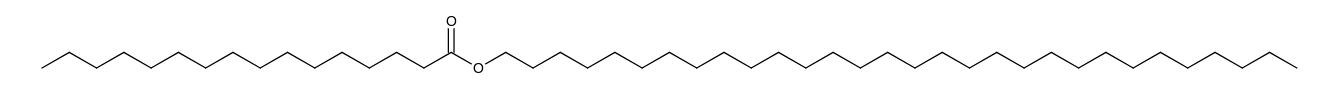
\includegraphics{smile-540e060fe3678bd7c83941f28ee462932ff24b0e}

myricyl palmitate\\
1.22. a)\\
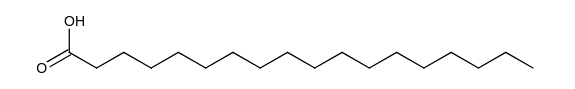
\includegraphics{smile-fcada1d664f81e415c0b420d6c448a01c45a27dc}

stearic acid\\
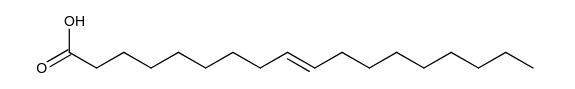
\includegraphics{smile-f855672583878fcd318c0e47e4f9100d28a50c2b}\\
b) Oleic acid có liên kết đôi $\mathrm{C}=\mathrm{C}$ ở dạng cis, zigzag hơn stearic acid là acid béo no. Do đó các phân tử stearic acid trong mạng tinh thể xếp khít với nhau hơn so với oleic acid. Kết quả là lực hút giữa các phân tử stearic acid mạnh hơn so với oleic acid làm cho nhiệt độ nóng chảy của stearic acid ( $69^{\circ} \mathrm{C}$ ) cao hon oleic acid ( $13,4^{\circ} \mathrm{C}$ ).\\
1.23. a) Công thức cấu tạo của tripalmitin, tristearin và triolein lần lượt là $\left(\mathrm{C}_{15} \mathrm{H}_{31} \mathrm{COO}\right)_{3} \dot{\mathrm{C}}_{3} \mathrm{H}_{5},\left(\mathrm{C}_{17} \mathrm{H}_{35} \mathrm{COO}\right)_{3} \mathrm{C}_{3} \mathrm{H}_{5}$ và $\left(\mathrm{C}_{17} \mathrm{H}_{33} \mathrm{COO}\right)_{3} \mathrm{C}_{3} \mathrm{H}_{5}$.\\
b) Dầu olive có hàm lượng các gốc acid béo không no cao, còn dầu ca cao có tổng hàm lượng các gốc acid béo no cao. Do đó ở điều kiện thường, dầu olive ở thể lỏng còn dầu ca cao lại ở thể rắn, có nghĩa là dầu olive có nhiệt độ đông đặc thấp hơn $\left(-6^{\circ} \mathrm{C}\right)$ so với dầu ca cao $\left(34^{\circ} \mathrm{C}\right)$.\\
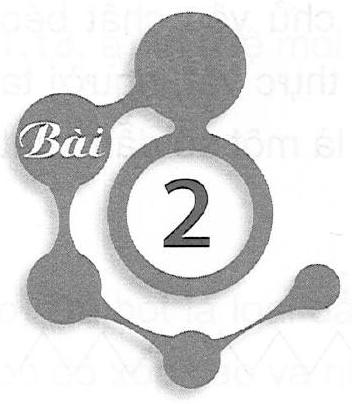
\includegraphics[max width=\textwidth, center]{2025_10_23_b4e16b74380d0f7e7700g-007}

\section*{XÀ PHÒNG VÀ CHẤT GIẶT RỦA}
2.1. Đáp án C .\\
2.2. Đáp án C.\\
2.3. Đáp án B. Nước bồ kết và dầu gội đầu có thành phần là các chất giặt rửa tự nhiên, tổng hợp.\\
2.4. Đáp án $C$.\\
2.5. Đáp án A. Sodium laurylsulfate là chất giặt rửa tổng hợp.\\
2.6.

\begin{center}
\begin{tabular}{|l|l|l|}
\hline
\multicolumn{1}{|c|}{Phân tử} & \multicolumn{1}{|c|}{Tên gọi} & \multicolumn{1}{|c|}{Phân loại} \\
\hline
$\mathrm{CH}_{3}\left[\mathrm{CH}_{2}\right]_{14} \mathrm{COOK}^{-}$ & potassium palmitate & Xà phòng \\
\hline
$\mathrm{CH}_{3}\left[\mathrm{CH}_{2}\right]_{11} \mathrm{OSO}_{3} \mathrm{Na}$ & \begin{tabular}{l}
sodium laurylsulfate \\
(hay sodium dodecylsulfate) \\
\end{tabular} & \begin{tabular}{l}
Chất giặt rừa \\
tồng hợp \\
\end{tabular} \\
\hline
$\mathrm{CH}_{3}\left[\mathrm{CH}_{2}\right]_{11} \mathrm{C}_{6} \mathrm{H}_{4} \mathrm{SO}_{2} \mathrm{ONa}$ & sodium 4-dodecylbenzenesulfonate & \begin{tabular}{l}
Chất giặt rửa \\
tông hợp \\
\end{tabular} \\
\hline
\end{tabular}
\end{center}

2.7. Chất giặt rửa tổng hợp không phải là xà phòng vì chúng không phải là muối sodium hoặc potassium của các acid béo. Tuy nhiên, chất giặt rửa tổng hợp cũng có hình mẫu của xà phòng, gồm một đầu ưa nước\\
gắn với một đuôi kị nước. Tương tự như xà phòng, chất giặt rửa tổng hợp cũng dùng để tắm gội, giặt giũ, ... dưới dạng dầu gội, sữa tắm, ... Chính vì vậy, chất giặt rửa tổng hợp "không phải xà phòng nhưng thường được gọi là xà phòng".\\
2.8. Khi cho xà phòng hoặc chất giặt rửa vào nước, đầu ưa nước sẽ bị hút vào các phân tử nước. Các phân tử xà phòng hoặc chất giặt rửa này tích tụ trên bề mặt nước với phần đầu ở trong nước và phần đuôi thẳng lên trong không khí, phá vỡ liên kết hydrogen giữa các phân tử nước, làm giảm sức căng bề mặt của nước, giúp nước dễ làm ướt các vật dụng và bám dính vào các vật mà nó tiếp xúc dễ hơn. Nhờ đó, nước dễ lan ra một diện tích rộng hơn và thấm sâu vào các sợi vải trong quá trình giặt.\\
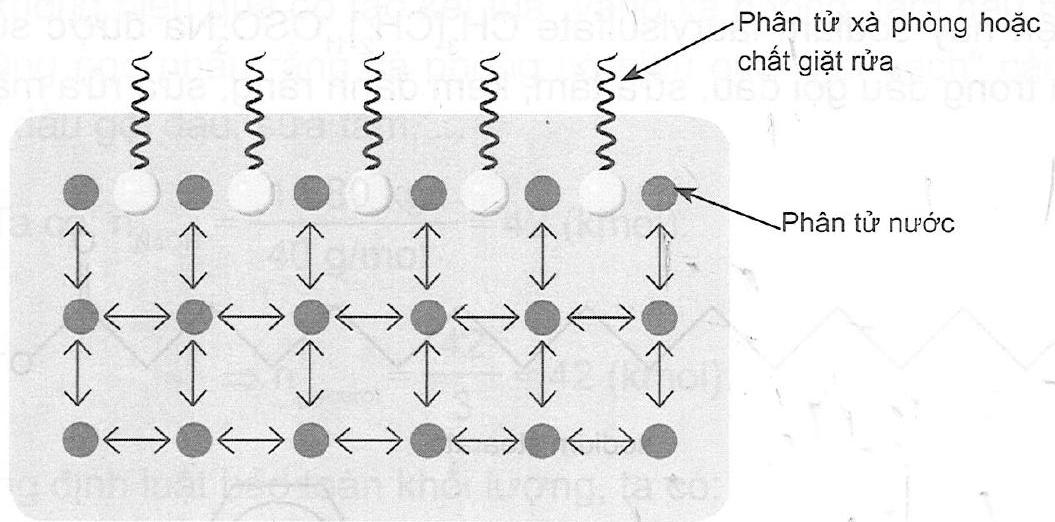
\includegraphics[max width=\textwidth, center]{2025_10_23_b4e16b74380d0f7e7700g-008}\\
2.9. Xà phòng diệt khuẩn là xà phòng được thêm một số chất kháng khuẩn khác, phổ biến là triclosan. Theo Cơ quan Quản lí Thực phẩm và Dược phẩm Mỹ (FDA), hiện tại vẫn không có đủ bằng chứng khoa học để chứng minh xà phòng diệt khuẩn có khả năng ngăn ngưa bệnh tật tốt hơn so với xà phòng thông thường. Ngoài ra, việc sử dụng rộng rãi xà phòng diệt khuẩn trong một thời gian dài có khả năng ảnh hưởng tiêu cực đến sức khoẻ của người sử dụng, do xảy ra khả năng kháng thuốc của các loại vi khuẩn, chưa kể còn tiêu diệt một số loài vi khuẩn có ích cho da. Vì thế, không nên lạm dụng việc sử dụng xà phòng diệt khuẩn trong rửa tay sát khuẩn.\\
2.10. Khi rửa tay sát khuẩn, alcohol có thể tiện sử dụng hơn. Tuy nhiên, xà phòng cũng như alcohol đều có khả năng diệt khuẩn do có thể hoà tan lớp vỏ lipid của vi khuẩn. Do đó, xà phòng cũng có công dụng rửa tay sát khuẩn, chưa kể còn giúp tiết kiệm chi phí.\\
2.11. a) Cả hai đều là muối sodium với đuôi dài kị nước và đầu ưa nước tích điện âm, trong đó một muối là sulfate và muối còn lại là sulfonate. Tuy nhiên, phân tử muối sulfate có đuôi không phân nhánh, còn phân tử muối sulfonate có mạch đuôi phân nhánh.\\
b) Trước đây, phân tử chất giặt rửa tổng hợp có đuôi phân nhánh như chất đã nêu ở trên được sử dụng một cách phổ biến. Tuy nhiên vì chúng khó bị phân huỷ sinh học nên đã gây ra nhiều bọt ở sông, bờ biển, hồ và hệ thống nước thải cũng như gây ô nhiễm nguồn cung cấp nước uống. Các chất giặt rửa tổng hợp có mạch không phân nhánh phân huỷ sinh học dễ dàng hơn nhiều, vì vậy chúng đã thay thế phần lớn các chất giặt rửa tổng hợp có mạch phân nhánh.

Ví dụ hiện nay sodium laurylsulfate $\mathrm{CH}_{3}\left[\mathrm{CH}_{2}\right]_{11} \mathrm{OSO}_{3} \mathrm{Na}$ được sử dụng phổ biến trong dầu gội đầu, sữa tắm, kem đánh răng, sữa rửa mặt, ...\\
2.12. a)\\
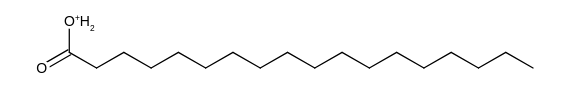
\includegraphics{smile-a810cbe4b7b7e4dff4512c1992550588e1047561}

sodium stearate\\
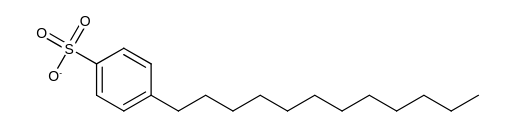
\includegraphics{smile-683f445d4e98433383d6322cb1565dc69f146669}

sodium 4-dodecylbenzenesulfonate\\
b) Cả hai đều là muối sodium với đuôi dài kị nước và đầu ưa nước tích điện âm. Tuy nhiên, sodium stearate là muối carboxylate, trong khi sodium 4-dodecylbenzenesulfonate là muối sulfonate.\\
Nguyên tắc làm sạch của chúng đều giống nhau: đuôi dài kị nước nhưng ưa dầu thâm nhập vào vết bẩn dầu mỡ và nhờ các đầu ưa nước kéo các vết bẩn này vào nước.\\
c) Trong nước cứng, sodium stearate mất khả năng giặt rửa do tạo muối khó tan là calcium stearate hoặc magnesium stearate, còn sodium 4-dodecylbenzenesulfonate không mất tính giặt rửa do không tạo muối khó tan với $\mathrm{Ca}^{2+}, \mathrm{Mg}^{2+}$.\\
2.13. a) Chất giặt rửa anion là chất giặt rửa mà phân tử có đuôi dài kị nước gắn với một đầu anion ưa nước như sodium 4-dodecylbenzenesulfonate $\left[\mathrm{CH}_{3}\left(\mathrm{CH}_{2}\right)_{11} \mathrm{C}_{6} \mathrm{H}_{4} \mathrm{SO}_{3}\right]-\mathrm{Na}^{+}$hay sodium laurylsulfate $\left[\mathrm{CH}_{3}\left(\mathrm{CH}_{2}\right)_{11} \mathrm{OSO}_{3}\right]-\mathrm{Na}^{+}, \ldots$ Gọi là chất giặt rửa anion để phân biệt với chất giặt rửa cation. Chất giặt rửa cation là chất giặt rửa mà phân tử có đuôi dài kị nước gắn với một đầu cation ưa nước như dodecylamine hydrochloride $\left[\mathrm{CH}_{3}\left(\mathrm{CH}_{2}\right)_{11} \mathrm{NH}_{3}\right]^{+} \mathrm{Cl}^{-}$.\\
b) Chất giặt rửa anion được phát minh vào những năm 1930. Xà phòng và chất giặt rửa anion hoạt động theo cùng một cách để làm sạch và loại bỏ các vết bẩn. Tuy nhiên so với nhóm sulfonate trong chất giặt rửa anion, nhóm carboxylate trong xà phòng rất dễ tạo kết tủa với các cation có trong nước máy như $\mathrm{Ca}^{2+}$ và $\mathrm{Mg}^{2+}$. Khi điều này xảy ra, xà phòng hoạt động không hiệu quả do tạo kết tủa "váng xà phòng" làm hầu hết người tiêu dùng ngộ nhận rằng xà phòng có hiệu quả "gột sạch" các vết bẩn hơn là dầu gội đầu, sữa tắm, ...\\
2.14. Ta có: $\mathrm{n}_{\mathrm{NaOH}}=\frac{1680 \mathrm{~kg}}{40 \mathrm{~g} / \mathrm{mol}}=42(\mathrm{kmol})$.

$$
\Rightarrow \mathrm{n}_{\text {glycerol }}=\frac{42}{3}=42(\mathrm{kmol}) .
$$

Áp dụng định luật bảo toàn khối lượng, ta có:

$$
\begin{aligned}
m_{\text {muối }} & =m_{\text {chất béo }}+m_{\mathrm{NaOH}}-m_{\text {glycerol }} \\
& =10000+1680-14 \times 92 \\
& =10392(\mathrm{~kg}) .
\end{aligned}
$$

Nhưng khối lượng muối sodium carboxylate chiếm 65\% khối lượng xà phòng nên thực tế khối lượng xà phòng thu được là:

$$
\mathrm{m}=\frac{10392 \times 100}{65} \approx 15988(\mathrm{~kg})
$$

2.15. Ta có: $\mathrm{n}_{\mathrm{KOH} \text { (đä düng) }}=1 \mathrm{~mol}$ và $\mathrm{n}_{\text {glycerol }}=0,32 \mathrm{~mol}$.

Điều này chứng tỏ chất béo $A$ đã cho gồm các triglyceride có lẫn một phần acid béo.\\
Định luật bảo toàn khối lượng cho:

$$
\begin{aligned}
& m_{A}+m_{\mathrm{KOH}}=m_{\text {muối }}+m_{\text {glycerol }}+m_{\text {nước }} \\
& \Rightarrow m_{\text {muối }}=\left(m_{A}+m_{\mathrm{KOH}}\right)-\left(m_{\text {glycerol }}+m_{\text {nước }}\right) \\
& =(300+1 \times 56)-[92 \times 0,32+18 \times(1-3 \times 0,32)]=325,84(\mathrm{~g}) .
\end{aligned}
$$

Do khối lượng muối sodium carboxylate chiếm $70 \%$ khối lượng xà phòng nên thực tế khối lượng xà phòng thu được là:

$$
\mathrm{m}=\frac{325,84 \times 100}{70} \approx 465,5(\mathrm{~g}) .
$$

2.16. Trong 2 ngày đầu tiên, khối lượng bánh xà phòng giảm nhanh nhất, căn cứ trên biểu đồ là khoảng 5 g . Trong những chu kì 2 ngày tiếp theo, khối lượng bánh xà phòng tiếp tục giảm nhưng không giảm nhanh như 2 ngày đầu tiên, mức độ giảm chậm dần. Ở 4 ngày cuối, khối lượng bánh xà phòng hầu như không đổi, ổn định ở mức 90 g .\\
Từ dữ kiện đã cho, tính ra kể từ sau điều chế 14 ngày, khối lượng bánh xà phòng hầu như ổn định. Độ hao hụt khối lượng là $\frac{100-90}{100}=10 \%$.\\
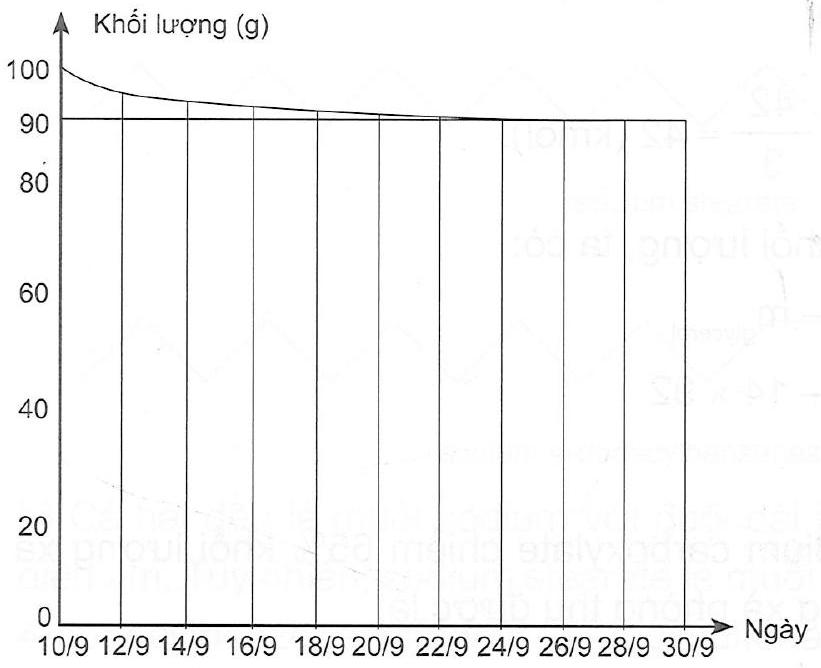
\includegraphics[max width=\textwidth]{2025_10_23_b4e16b74380d0f7e7700g-011} nhiệt, lượng nước những ngày đầu bốc hơi nhanh hơn những ngày sau đó. Khi phản ứng xà phòng hoá đã xảy ra xong, khối lượng bánh xà phòng cơ bản thay đổi không đáng kể.\\
2.17. Trong xét nghiệm Hay (Hay's test), bột lưu huỳnh được rắc vào ống nghiệm chứa 3 mL nước tiểu. Do có sự hiện diện của các muối mật, nước tiểu của người bị bệnh về gan có sức căng bề mặt giảm so với nước tiểu của người bình thường, vì thế khi được rắc lên bề mặt nước

Những ngày đầu, khối lượng xà phòng giảm nhanh hơn so với những ngày sau là do trong phương pháp làm lạnh, phản ứng xà phòng hoá vẫn đang diễn ra trong quá trình bảo quản bánh xà phòng và điều này thể hiện trong báo cáo kết quả thực hành của nhóm. Do phản ứng xà phòng hoá là phản ứng toả đó. Khi phản ứng xà phòng hoá đã xảy ra xong, khối lượng bánh xà\\
phòng cơ bản thay đồi không đáng kê. 2.17. Trong xét nghiệm Hay (Hay's test), bột lưu huỳnh được rắc vào ống nghiệm chứa 3 mL nước tiểu. Do có sự hiện diện của các muối mật, nước tiểu của người bị bệnh về gan có sức căng bề mặt giảm so với nước tiểu của người bình thường, vì thế khi được rắc lên bề mặt nước\\
tiểu, bột lưu huỳnh sẽ nổi lên đối với nước tiểu của người bình thường và chìm xuống đối với nước tiểu của người mắc bệnh gan.\\
2.18. Nước nóng có sức căng bề mặt giảm hơn so với nước lạnh, do đó nước nóng giúp nước dễ làm ướt và bám dính vào các vật mà nó tiếp xúc. Nhờ đó, nước nóng dễ lan ra một diện tích rộng và thấm sâu vào các sợi vải trong quá trình giặt, giúp quần áo được giặt sạch hơn. Ngoài ra, nước nóng có khả năng phân huỷ hoặc làm bay hơi các phân tử màu nên quần áo giặt bằng nước nóng sẽ sạch hơn so với giặt bằng nước lạnh.\\
2.19. Khi rửa tay bằng xà phòng hoặc chất giặt rửa tổng hợp, màng chất béo bao bọc tế bào virus hoặc vi khuẩn sẽ bị hoà tan bởi xà phòng hoặc chất giặt rửa tổng hợp, lộ ra các thành phần quan trọng bên trong tế bào làm cho vi khuẩn, virus nhanh chóng bị bất hoạt.\\
2.20. Các mẫu thí nghiệm được tiến hành ở 3 nhiệt độ khác nhau, với mục đích xác định độ hoạt động tối ưu của protease ở các nhiệt độ khảo sát. Trên biểu đồ, tốc độ phân huỷ chất bẩn đạt mức cao nhất là 12,5 $\mu \mathrm{mol} /$ phút $0^{3} 40^{\circ} \mathrm{C}$ nên độ hoạt động của protease trong thí nghiệm là tối ưu ở nhiệt độ trên.\\
2.21. Khi sử dụng xà phòng chung với giấm ăn, xà phòng sẽ mất khả năng giặt rửa do xảy ra phản ứng tạo thành acid béo khó tan trong nước.\\
Ví dụ khi sử dụng xà phòng sodium stearate chung với giấm ăn sẽ xảy ra phản ứng tạo thành stearic acid khó tan, làm xà phòng mất tính giặt rửa:\\
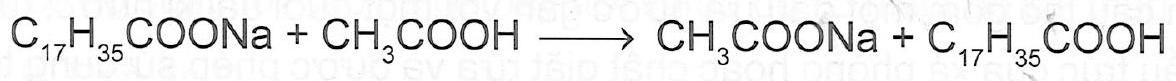
\includegraphics[max width=\textwidth, center]{2025_10_23_b4e16b74380d0f7e7700g-012}\\
2.22. Dung dịch NaCl bão hoà có tác dụng làm xà phòng kết tủa triệt để. Do dung dịch NaCl bão hoà có khối lượng riêng $\left(1,20 \mathrm{~g} / \mathrm{cm}^{3}\right)$ lớn hơn so với xà phòng $\left(1,01-1,10 \mathrm{~g} / \mathrm{cm}^{3}\right)$ nên xà phòng tạo thành nổi lên trên. Chú ý khối lượng riêng của dung dịch NaCl tỉ lệ thuận với nồng độ dưng dịch nên dung dịch NaCl bão hoà có khối lượng riêng lớn, giúp xà phòng dễ nổi trong dung dịch hơn so với dung dịch NaCl chưa bão hoà.\\
2.23. Xà phòng làm giảm sức căng bề mặt của nước, nhờ đó bong bóng nước xà phòng bền và không vỡ. Chính vì vậy, chỉ có thể thổi bong bóng với nước xà phòng mà không thể thổi bong bóng với nước sạch.\\
Điều thú vị là em có thể tạo một mái vòm bong bóng giống như sơ đồ bên dưới bằng cách làm ướt bề mặt một chiếc mâm lớn với nước xà phòng.

Dùng ống hút thổi một bong bóng nước xà phòng lớn nhất có thể. Đẩy ống hút qua bong bóng ban đầu và thổi một bong bóng khác nhỏ hơn vào bên trong và tiếp tục lặp lại các bước tương tự. Thử xem kỉ lục của em là tạo được bao nhiêu mái vòm bong bóng.\\
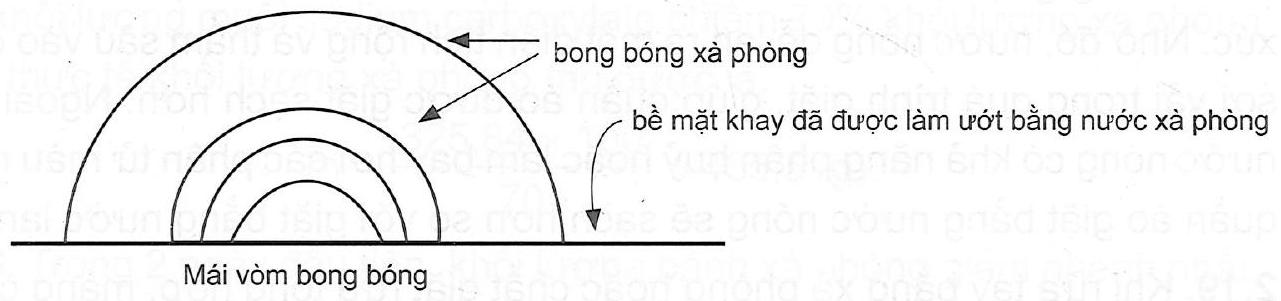
\includegraphics[max width=\textwidth, center]{2025_10_23_b4e16b74380d0f7e7700g-013}\\
2.24*. a) Lòng đỏ trứng đóng vai trò chất tạo nhũ trong quá trình chế biến.\\
b) Chất nhũ hoá ở đây là lòng đỏ trứng, hoạt động bằng cách làm giảm sức căng bề mặt giữa các phân tử dầu và nước, cho phép chúng trộn lẫn và tạo thành một hỗn hợp ổn định, đồng nhất, gọi là nhũ tương.\\
c) Lòng đỏ trứng được tạo thành từ nước, protein, chất béo và nhiều chất khác, bao gồm lecithin và cholesterol. Lecithin là một loại lipid được tìm thấy với nồng độ cao trong lòng đỏ trứng và là hợp chất mang lại đặc tính nhũ hoá cho lòng đỏ trứng.\\
Lecithin là một hợp chất có đuôi kị nước và một đầu ưa nước, tức "vừa ưa dầu, vừa ưa nước" nên đã mang lại đặc tính nhũ hoá cho lòng đỏ trứng. Nhờ đó, lecithin trở thành một chất nhũ hoá trong chế biến thực phẩm. Như vậy, chất được sử dụng thay thế lòng đỏ trứng ở trên phải có đặc điểm cấu tạo gồm một đầu ưa nước gắn với một đuôi dài kị nước, tương tự cấu trúc của xà phòng hoặc chất giặt rửa và được phép sử dụng trong chế biến thực phẩm.\\
d) Hợp chất đã cho có khả năng sử dụng làm chất nhũ hoá do có một đầu ưa nước gắn với một đuôi dài kị nước, tức có đặc tính "vừa ưa dầu, vừa ưa nước".

\begin{figure}[h]
\begin{center}
  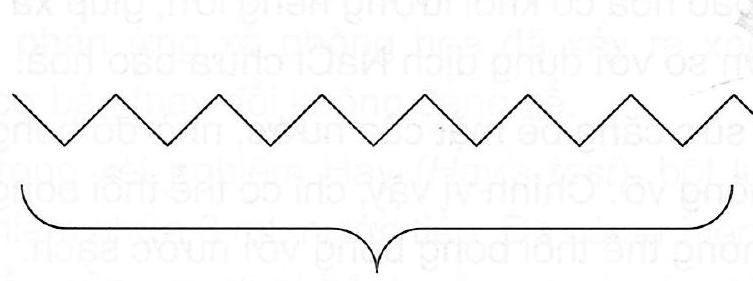
\includegraphics[width=\textwidth]{2025_10_23_b4e16b74380d0f7e7700g-013(1)}
\captionsetup{labelformat=empty}
\caption{Đuôi dài kị nước}
\end{center}
\end{figure}

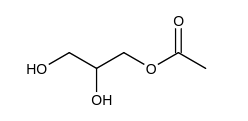
\includegraphics{smile-f69f5025ca38680a2e5e34a5b4a069e29f561f3b}

Đầu ưa nước

\section*{ÔN TẬP CHUONG 1}
OT1.1. Đáp án D.\\
OT1.4. Đáp án D.\\
OT1.7. Đáp án D.

OT1.2. Đáp án D. OT1.3. Đáp án D.\\
OT1.5. Đáp án A . OT1.6. Đáp án B.

Ta có phương trình nhiệt hoá học của các phản ứng:

$$
\begin{array}{ll}
2 \mathrm{C}(\mathrm{~s})+\mathrm{O}_{2}(\mathrm{~g})+2 \mathrm{H}_{2}(\mathrm{~g}) \xrightarrow{\mathrm{t}^{\circ}} \mathrm{HCOOCH}_{3}(\mathrm{l}) & \Delta_{\mathrm{r}} \mathrm{H}_{298}^{\circ}=\mathrm{a} \\
\mathrm{HCOOCH}_{3}(\mathrm{l})+2 \mathrm{O}_{2}(\mathrm{~g}) \xrightarrow{\mathrm{t}^{\circ}} 2 \mathrm{CO}_{2}(\mathrm{~g})+2 \mathrm{H}_{2} \mathrm{O}(\mathrm{~g}) & \Delta_{\mathrm{r}} \mathrm{H}_{298}^{\circ}=\mathrm{b} \\
2 \mathrm{CO}_{2}(\mathrm{~g}) \xrightarrow{\mathrm{t}^{\circ}} 2 \mathrm{C}(\mathrm{~s})+2 \mathrm{O}_{2}(\mathrm{~g}) & \Delta_{\mathrm{r}} \mathrm{H}_{298}^{\circ}=-2 \mathrm{c}
\end{array}
$$

Cộng 3 phản ứng trên, kết quả được:

$$
2 \mathrm{H}_{2}(\mathrm{~g})+\mathrm{O}_{2}(\mathrm{~g}) \xrightarrow{\mathrm{t}^{\circ}} 2 \mathrm{H}_{2} \mathrm{O}(g) \quad \Delta_{\mathrm{r}} \mathrm{H}_{298}^{\circ}=\mathrm{a}+\mathrm{b}-2 \mathrm{c}
$$

Theo đề, ta cũng có:

$$
2 \mathrm{H}_{2}(\mathrm{~g})+\mathrm{O}_{2}(\mathrm{~g}) \xrightarrow{\mathrm{t}^{\circ}} 2 \mathrm{H}_{2} \mathrm{O}(\mathrm{~g}) \quad \Delta_{\mathrm{r}} \mathrm{H}_{298}^{\circ}=2 \mathrm{~d}
$$

Vậy $2 \mathrm{~d}=\mathrm{a}+\mathrm{b}-2 \mathrm{c}$.\\
OT1.8. Đáp án B.\\
Chất có áp suất hơi cao thì dễ bay hơi và do đó có nhiệt độ sôi thấp hơn.\\
OT1.9. Đáp án D.\\
OT1.10. a) Ta có $\% \mathrm{O}=100 \%-(40,7 \%+5,1 \%)=54,2 \%$.\\
Đặt công thức của $X$ là $\mathrm{C}_{x} \mathrm{H}_{y} \mathrm{O}_{z}$, ta có:

$$
x: y: z=\frac{\% C}{12}: \frac{\% H}{1}: \frac{\% O}{16}=\frac{40,7}{12}: \frac{5,1}{1}: \frac{54,2}{16}=3,39: 5,10: 3,39=2: 3: 2
$$

Vậy công thức thực nghiệm của X là $\mathrm{C}_{2} \mathrm{H}_{3} \mathrm{O}_{2}$.\\
b) Dựa vào phổ khối của $X$, nhận thấy phân tử khối của $X$ là 118 , do đó $X$ có công thức phân tử là $\mathrm{C}_{4} \mathrm{H}_{6} \mathrm{O}_{4}$.\\
c) $X$ có thể có các công thức cấu tạo:

$$
\mathrm{HOOCCH}_{2} \mathrm{CH}_{2} \mathrm{COOH} \text { hoặc } \mathrm{CH}_{3} \mathrm{CH}(\mathrm{COOH})_{2}
$$

d) 20 g dung dịch Y chứa 1 g chất X nên khối lượng chất X có trong 4 g dung dịch $Y$ là:

$$
m_{x}=\frac{4}{20}=0,2(g)
$$

Do $\mathrm{n}_{\mathrm{NaOH}}=0,017 \times 0,2=0,0034(\mathrm{~mol})$.\\
Nên $\mathrm{n}_{\mathrm{x}}=\frac{0,0034}{2}=0,0017(\mathrm{~mol})$.\\
Vậy $\mathrm{M}_{\mathrm{x}}=\frac{0,2}{0,0017}=117,6$.\\
e) Vì $Z$ không phân nhánh nên $X$ phải không phân nhánh.

Vậy công thức cấu tạo của $X$ là $\mathrm{HOOC}-\mathrm{CH}_{2} \mathrm{CH}_{2}-\mathrm{COOH}$, có tên succinic acid.\\
$Z$ là ester của $X$ với ethanol nên công thức cấu tạo của $Z$ là $\mathrm{C}_{2} \mathrm{H}_{5} \mathrm{OOC}-\mathrm{CH}_{2} \mathrm{CH}_{2}-\mathrm{COOC}_{2} \mathrm{H}_{5}$, có tên diethyl succinate.\\
Phương trình hoá học của phản ứng:\\
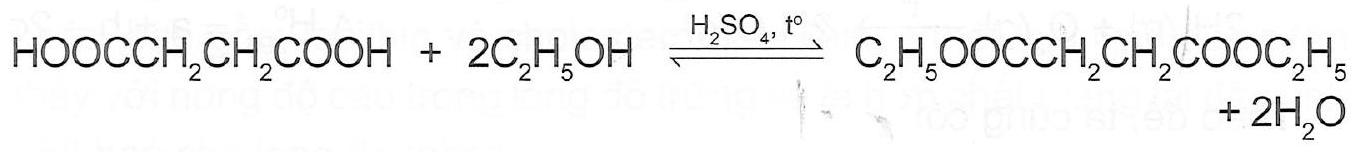
\includegraphics[max width=\textwidth, center]{2025_10_23_b4e16b74380d0f7e7700g-015}\\
g) Trước hết, cho dung dịch NaOH dư vào hỗn hợp sau phản ứng, toàn bộ succinic acid chuyển thành muối disodium succinate. Sau đó, thêm dung môi hexane vào, diethyl succinate sẽ tan trong hexane, còn ethanol, disodium succinate và sodium hydroxide tan trong nước. Dùng phễu chiết để tách lớp hexane có hoà tan diethyl succinate.\\
Do hexane và diethyl succinate có nhiệt độ sôi chênh lệch nhiều ( $68,7^{\circ} \mathrm{C}$ so với $217^{\circ} \mathrm{C}$ ) nên có thể dùng phương pháp chưng cất để tách riêng chúng.\\
OT1.11. a) Công thức khung phân tử của elaidic acid và oleic acid lần lượt là:\\
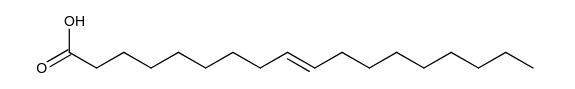
\includegraphics{smile-22696f0883bb4885950955b0f3baa2636607dbfa}

elaidic acid\\
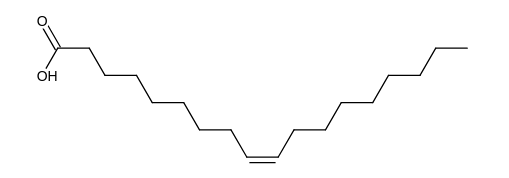
\includegraphics{smile-bd02b89272428b67383050cd4a9dcf0ee552f838}

oleic acid\\
b) Oleic acid và elaidic acid là đồng phân hình học của nhau, trong đó oleic acid có liền kết đôi $\mathrm{C}=\mathrm{C}$ ở dạng cis nên zigzag hơn elaidic acid có liên kết đôi $\mathrm{C}=\mathrm{C}$ ở dạng trans.\\
c) Do oleic acid có liên kết đôi $\mathrm{C}=\mathrm{C}$ ở dạng cis, zigzag hơn elaidic acid có liên kết đôi $\mathrm{C}=\mathrm{C}$ ở dạng trans nên các phân tử elaidic acid trong mạng tinh thể xếp khít với nhau hơn so với oleic acid. Kết quả là lực hút giữa các phân tử elaidic acid mạnh hơn so với oleic acid làm nhiệt độ nóng chảy của elaidic acid ( $45^{\circ} \mathrm{C}$ ) cao hơn so với oleic acid ( $13,4^{\circ} \mathrm{C}$ ).\\
OT1.12. Do $Y$ có nhiệt độ sôi cao hơn $X$ nên $Y$ là carboxylic acid và $X$ là ester, ứng với các công thức cấu tạo:

$$
\begin{aligned}
& \mathrm{X} \text { là } \mathrm{HCOO}-\mathrm{CH}=\mathrm{CH}_{2} \\
& \mathrm{Y} \text { là } \mathrm{CH}_{2}=\mathrm{CH}-\mathrm{COOH}
\end{aligned}
$$

OT1.13. a) Acid béo rất quan trọng cho hoạt động bình thường của tất cả các hệ thống trong cơ thể như hệ thống tuần hoàn, hệ thống hô hấp, hệ thống miễn dịch, não và các cơ quan khác. Cơ thể có khả năng tổng hợp hầu hết các acid béo từ thức ăn, những acid béo này được gọi là acid béo không thiết yếu. Ngoài ra, có một số acid béo cơ thể không thể tổng hợp được, chúng được gọi là acid béo thiết yếu. Cần lưu ý acid béo không thiết yếu thì không có nghĩa là không quan trọng, việc phân loại nêu trên chỉ dựa vào khả năng tổng hợp acid béo của cơ thể.\\
Acid béo thiết yếu phải được lấy từ thực phẩm, chúng thuộc hai loại là omega-3 và omega-6. Acid béo omega-3 và omega-6 là tiền thân của các hợp chất quan trọng, được gọi là eicosanoid. Eicosanoid là những hormone kiểm soát nhiều hormone khác và các chức năng quan trọng của cơ thể như hệ thống thần kinh trung ương, hệ thống miễn dịch. Do đó trong số 3 acid béo đã cho, chỉ có linoleic acid là acid béo thiết yếu.\\
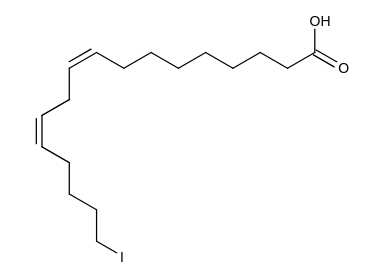
\includegraphics{smile-f7d062b4ad83a9c8dd37a4cfa49ce8f46755cf7f}

Linoleic acid là acid béo omega-6\\
b) Nhiệt độ nóng chảy của 3 acid béo đã cho có liên quan đến cấu trúc phân tử của chúng.\\
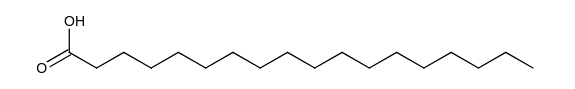
\includegraphics{smile-2a132e8d083b45345ea11411dc5cc8586c2e841e}

stearic acid\\
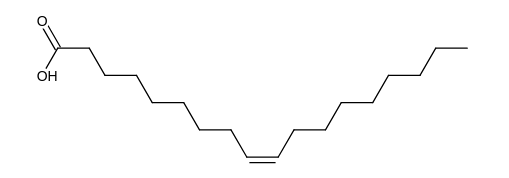
\includegraphics{smile-a31f3f8f63a3436209e87cd734e7dda04fa9d291}

oleic acid\\
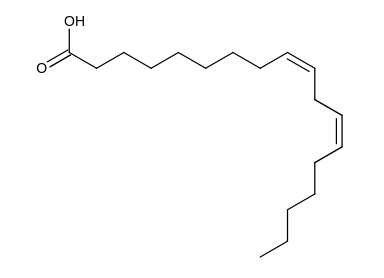
\includegraphics{smile-cf2e3d07a1acd9985c0b97107fd7089cd992f3e3}

linoleic acid

Ta đã biết liên kết đôi $\mathrm{C}=\mathrm{C}$ ở dạng cis làm phân tử trở nên zigzag nhiều hơn. Stearic acid là acid béo no có cấu trúc ít ziggag nhất, còn oleic acid có 1 liên kết đôi $\mathrm{C}=\mathrm{C}$ ở dạng cis và linoleic acid có 2 liên kết đôi $\mathrm{C}=\mathrm{C}$ ở dạng cis nên oleic acid có cấu trúc zigzag nhiều hơn và linoleic acid có cấu trúc zigzag nhất.\\
Điều này dẫn đến các phân tử stearic acid trong mạng tinh thể xếp khít với nhau nhất, rồi đến oleic acid và linoleic acid là kém khít nhất. Kết quả là lực hút giữa các phân tử acid béo giảm dần theo thự tự từ stearic acid đến linoleic acid, làm nhiệt độ nóng chảy của chúng giảm dần theo thứ tự trên theo bảng sau:

\begin{center}
\begin{tabular}{|c|c|c|c|}
\hline
Acid béo & stearic acid & oleic acid & linoleic acid \\
\hline
Nhiệt độ nóng chảy $\left({ }^{\circ} \mathrm{C}\right)$ & 69 & 13,4 & -5 \\
\hline
\end{tabular}
\end{center}

Ở điều kiện thường $\left(25^{\circ} \mathrm{C}\right)$, stearic acid ở thể rắn do có nhiệt độ nóng chảy là $69^{\circ} \mathrm{C}$, còn oleic acid và linoleic acid ở thể lỏng do có nhiệt độ nóng chảy lần lượt là $13,4^{\circ} \mathrm{C}$ và $-5^{\circ} \mathrm{C}$.\\
c) Phân tử muối sodium hoặc potassium của chúng đều có một đầu ưa nước gắn với một đuôi dài kị nước nên đều được sử dụng làm xà phòng.

OT1.14. Động vật cũng tạo ra chất sáp đóng vai trò là lớp phủ bảo vệ, giữ cho bề mặt của lông, da không thấm nước. Trên thực tế, nếu lớp sáp phủ trên lông của chim bị hoà tan do chim bơi trong vết dầu loang, lông của chúng sẽ trở nên ẩm ướt và nặng hơn làm chim không thể duy trì khả năng nổi trên nước, dẫn đến chúng bị chết đuối.

OT1.15. Khi sử dụng xà phòng RCOONa để giặt giũ, phân tử RCOONa tan trong nước, phân li ra ion $\mathrm{RCOO}^{-}$và $\mathrm{Na}^{+}$. Do đó, đầu ưa nước của phân tử xà phòng RCOONa là $-\mathrm{COO}^{-}$, không phải -COONa . Tuy nhiên để đơn giản, người ta thường nói đầu ưa nước của phân tử xà phòng RCOONa là -COONa .

OT1.16. a) Công thức khung phân tử của myricyl cerotate:\\
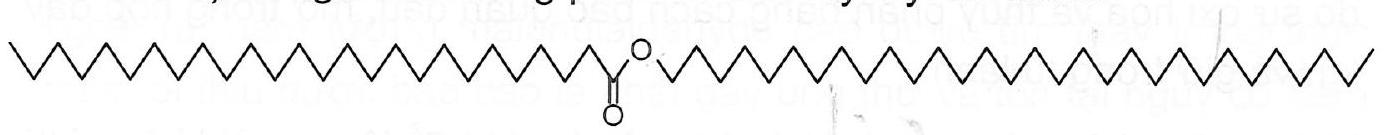
\includegraphics[max width=\textwidth, center]{2025_10_23_b4e16b74380d0f7e7700g-018}\\
b) Thực vật ngăn ngừa mất nước bằng cách phủ sáp trên bề mặt lá của chúng. Thành phần sáp thường khác nhau giữa các loài, các cơ quan và các giai đoạn phát triển của cây. Hàm lượng sáp trên lá tăng ở những khu vực có nhiệt độ cao hoặc có lượng bức xạ mặt trời lớn hay những vùng khô cằn, vùng có lượng nước trong đất thấp.

Ngoài việc làm giảm sự thoát hơi nước của lá, lớp sáp còn ngăn không cho nước và các hạt tích tụ trên bề mặt lá, ức chế sự phát triển của mầm bệnh.\\
OT1.17. a)\\
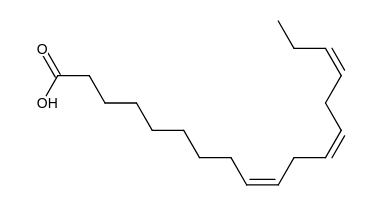
\includegraphics{smile-a4eac796d7dcd321079e4a4133957cc7d5106d67}

$\alpha$-linolenic acid\\
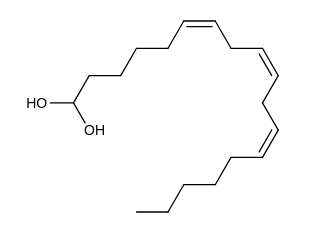
\includegraphics{smile-906eea08d16f2b61beb45066cae3e350f06241a7}

$\gamma$-linolenic acid\\
b) $\alpha$-linolenic acid là acid béo thuộc nhóm omega- 3 và $\gamma$-linolenic acid là acid béo thuộc nhóm omega- 6 nên chúng đều là các acid béo thiết yếu.\\
c) Liên kết đôi $\mathrm{C}=\mathrm{C}$ ở dạng cis làm phân tử trở nên zigzag nhiều hơn. Stearic acid là acid béo no có cấu trúc ít ziggag nên các phân tử của chúng trong mạng tinh thể xếp khít với nhau nhất so với $\alpha$-linolenic acid và $\gamma$-linolenic acid. Kết quả là lực hút giữa các phân tử stearic acid là mạnh nhất, làm cho nhiệt độ nóng chảy của stearic acid cao hơn các acid còn lại.

\begin{center}
\begin{tabular}{|c|c|c|c|}
\hline
Acid béo & stearic acid & $\alpha$-linolenic acid & $\gamma$-linolenic acid \\
\hline
Nhiệt độ nóng chảy $\left({ }^{\circ} \mathrm{C}\right)$ & 69 & $-16,5$ & $-11,3$ \\
\hline
\end{tabular}
\end{center}

OT1.18. a) Chất béo khi tiếp xúc với không khí ẩm ở nhiệt độ phòng sẽ xảy ra các phản ứng oxi hoá và thuỷ phân làm cho chúng bị phân huỷ, gây ôi thiu và tạo hợp chất có mùi khó chịu. Có thể ngăn ngừa sự ôi thiu do sự oxi hoá và thuỷ phân bằng cách bảo quản dầu, mỡ trong hộp đậy kín và giữ trong tủ lạnh.\\
b) Nguyên nhân gây ra mùi khó chịu của bơ khi để lâu ngoài không khí ẩm là do những vi sinh vật có trong không khí cung cấp lipase là enzyme xúc tác quá trình thuỷ phân bơ, tạo ra butyric acid có mùi khó ngửi.\\
c) Quan sát cấu trúc phân tử của linoleic acid và linolenic acid, ta thấy chúng đều chứa đoạn mạch carbon $-\mathrm{CH}=\mathrm{CH}-\mathrm{CH}_{2}-\mathrm{CH}=\mathrm{CH}-$ như sau:\\
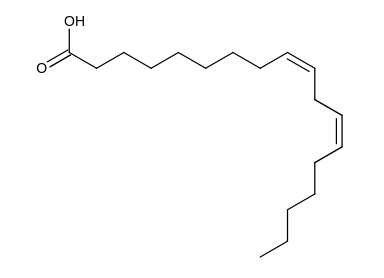
\includegraphics{smile-1a8ec449a9cb6da217b944a9b98b7de326691042}

linolenic acid\\
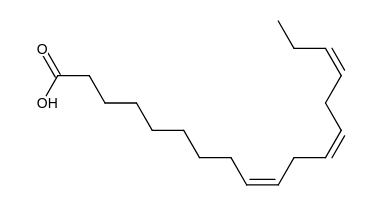
\includegraphics{smile-4c2496252ff15247b50bbfd5e3b00d95a212b740}\\
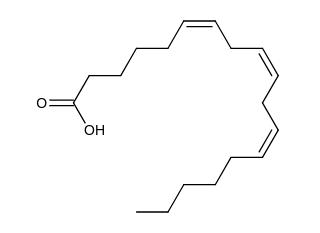
\includegraphics{smile-e55ca94492ca2fdcbcf52abd560638da1d8f75bb}

$\gamma$-linolenic acid

Khi 2 liên kết đôi trong đoạn mạch $-\mathrm{CH}=\mathrm{CH}-\mathrm{CH}_{2}-\mathrm{CH}=\mathrm{CH}-$ bị oxi hoá sẽ giải phóng MDंA. Điều đó giải thích vì sao các chất béo có chứa thành phần là linoleic acid hoặc $\alpha$-linolenic acid dễ bị oxi hoá tạo mùi khó chịu.\\
d) Chất chống oxi hoá là những hợp chất có ái lực với oxygen lớn hơn ái lực của lipid trong thực phẩm. Chúng hoạt động bằng cách ưu tiên làm cạn kiệt nguồn cung cấp oxygen được hấp thụ vào sản phẩm và được thêm vào với lượng rất nhỏ $(0,001 \%-0,01 \%)$ để giúp ngăn chặn quá trình oxi hoá chất béo.\\
e) Dầu mỡ ôi thiu tạo ra các hợp chất gây hại. Các hoá chất như peroxide và aldehyde có thể làm hỏng tế bào và góp phần gây xơ vữa động mạch. Các gốc tự do sinh ra từ dầu ôi thiu cũng có thể làm hỏng DNA trong tế bào, gây tổn thương động mạch và có khả năng gây ung thư.

Ngoài ra, hàm lượng malondialdehyde cao được tìm thấy trong thực phẩm ôi thiu được báo cáo là chất gây ung thư và tồn tại nguy cơ tiềm ẩn đối với sức khoẻ.

\begin{table}[h]
\begin{center}
\captionsetup{labelformat=empty}
\caption{OT1.19.}
\begin{tabular}{|l|l|l|}
\hline
Phát biểu & Đúng & Sai \\
\hline
a) Ester E có khối lượng phân tử là $\mathrm{M}=60$. & $\checkmark$ &  \\
\hline
b) E là ester của methyl alcohol. & $\checkmark$ &  \\
\hline
c) Nhiệt độ sôi của E cao hơn ethyl alcohol. &  & $\checkmark$ \\
\hline
d) Xà phòng hoá E bằng dung dịch NaOH thu được muối có công thức $\mathrm{CHO}_{2} \mathrm{Na}$. & $\checkmark$ &  \\
\hline
\end{tabular}
\end{center}
\end{table}

\begin{table}[h]
\begin{center}
\captionsetup{labelformat=empty}
\caption{OT1.20.}
\begin{tabular}{|l|c|c|}
\hline
\multicolumn{1}{|c|}{Phát biểu} & Đúng & Sai \\
\hline
a) Triglyceride X có tên gọi là tripalmitin. &  & $\checkmark$ \\
\hline
b) X là chất béo no, Y là chất béo không no. & $\checkmark$ &  \\
\hline
\end{tabular}
\end{center}
\end{table}

\begin{center}
\begin{tabular}{|l|c|c|}
\hline
c) $X, Y$ đều tan tốt trong nước. &  & $\checkmark$ \\
\hline
d) Hydrogen hoá $Y$ thu được $X$. & $\checkmark$ &  \\
\hline
\end{tabular}
\end{center}

OT1.21.

\begin{center}
\begin{tabular}{|l|l|l|}
\hline
Phát biểu & Đúng & Sai \\
\hline
a) Sodium palmitate và sodium laurylsulfate đều là thành phần chính của xà phòng. &  & $\checkmark$ \\
\hline
b) Sodium palmitate và sodium laurylsulfate đều có tính năng giặt rửa. & $\checkmark$ &  \\
\hline
c) Sodium palmitate và sodium laurylsulfate đều tạo muối khó tan trong nước cứng. &  & $\checkmark$ \\
\hline
d) Sodium palmitate và sodium laurylsulfate đều có đầu ưa nước gắn với đuôi kị nước. & $\checkmark$ &  \\
\hline
\end{tabular}
\end{center}

OT1.22.

\begin{center}
\begin{tabular}{|l|l|l|}
\hline
Phát biểu & Đúng & Sai \\
\hline
a) Do không tạo được liên kết hydrogen giữa các phân tử nên ester có nhiệt độ sôi thấp hơn nhiệt độ sôi của carboxylic acid và alcohol có cùng số nguyên tử carbon. & $\checkmark$ &  \\
\hline
b) Do có khả năng tạo liên kết hydrogen yếu với nước nên ester thường ît tan trong nước hơn so với carboxylic acid và alcohol có cùng số carbon. & $\checkmark$ &  \\
\hline
c) Carboxylic acid có nhiệt độ sôi cao hơn alcohol có cùng số nguyên tử carbon. & $\checkmark$ &  \\
\hline
d) Methanol có khả năng tan vô hạn trong nước. & $\checkmark$ &  \\
\hline
\end{tabular}
\end{center}

\begin{center}
\begin{tabular}{|c|c|c|c|c|c|c|}
\hline
Câu & OT1.23 & OT1.24 & OT1.25 & OT1.26 & OT1.27 & OT1.28 \\
\hline
Đáp án & 2 & 5 & 4 & 3,2 & 23,6 & 465,5 \\
\hline
\end{tabular}
\end{center}

OT1.23. Có 2 ester cần tìm là $\mathrm{CH}_{3} \mathrm{CH}_{2} \mathrm{CH}_{2} \mathrm{COOCH}_{3}$ và $\left(\mathrm{CH}_{3}\right)_{2} \mathrm{CHCOOCH}_{3}$.\\
OT1.24. Vì hợp chất có $M=60$ mà chỉ chứa các nguyên tố carbon, hydrogen, oxygen nên hợp chất này có thể có công thức phân tử là $\mathrm{C}_{3} \mathrm{H}_{8} \mathrm{O}$ hoặc $\mathrm{C}_{2} \mathrm{H}_{4} \mathrm{O}_{2}$.

\begin{itemize}
  \item Có 3 hợp chất hữu cơ đơn chức có công thức phân tử $\mathrm{C}_{3} \mathrm{H}_{8} \mathrm{O}$ là $\mathrm{CH}_{3} \mathrm{CH}_{2} \mathrm{CH}_{2} \mathrm{OH},\left(\mathrm{CH}_{3}\right)_{2} \mathrm{CHOH}$ và $\mathrm{C}_{2} \mathrm{H}_{5} \mathrm{OCH}_{3}$.
  \item Có 2 hợp chất hữu cơ đơn chức có công thức phân tử $\mathrm{C}_{2} \mathrm{H}_{4} \mathrm{O}_{2}$ là $\mathrm{HCOOCH}_{3}$ và $\mathrm{CH}_{3} \mathrm{COOH}$.
\end{itemize}

Vậy tổng cộng có 5 hợp chất hữu cơ đơn chức cần tìm.\\
OT1.25. Có 4 triglyceride cần tìm là:\\
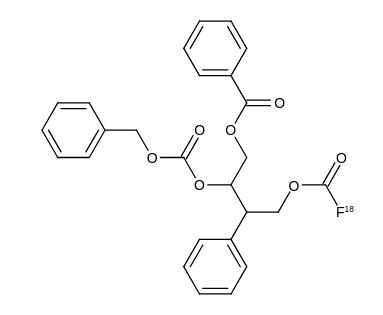
\includegraphics{smile-0bcaf2b156ad310a3e87a37ff8e3da907718e690}\\
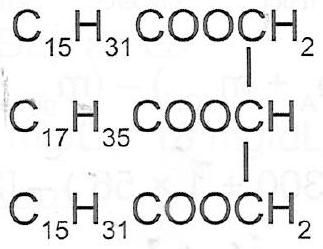
\includegraphics[max width=\textwidth, center]{2025_10_23_b4e16b74380d0f7e7700g-022(1)}\\
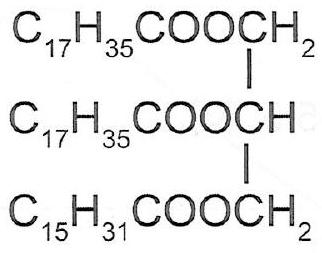
\includegraphics[max width=\textwidth, center]{2025_10_23_b4e16b74380d0f7e7700g-022}\\
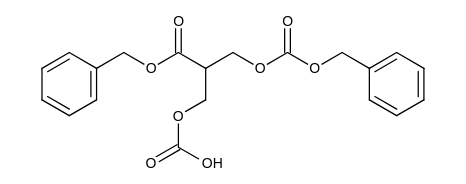
\includegraphics{smile-7ab118c0c8ea1ccb76756d5566478d28ef553197}

OT1.26. Đặt công thức ester là RCOOR'.\\
Theo đề, ta có $m_{\text {muói }}>m_{\text {ester }}$ nên $M_{R^{\prime}}<23 \Rightarrow M_{R^{\prime}}=15$.\\
Vậy ester E là methyl acetate, muối F là sodium acetate và alcohol G là methanol.\\
$\Rightarrow \mathrm{m}_{\mathrm{CH}_{3} \mathrm{OH}}=0,1 \times 32=3,2(\mathrm{~g})$.

OT1.27. Vì alcohol cháy cho số mol nước gấp đôi số mol $\mathrm{CO}_{2}$ nên alcohol là $\mathrm{CH}_{3} \mathrm{OH}$.

Do ester E có $\mathrm{M}<200$, xà phòng hoá tạo muối F , khi đốt F chỉ thu được $\mathrm{CO}_{2}$ và $0,2 \mathrm{~mol} \mathrm{Na}_{2} \mathrm{CO}_{3}$ cho thấy đây là muối $(\mathrm{COONa})_{2}$.

Vậy ester là $\left(\mathrm{COOCH}_{3}\right)_{2}$ và $n=0,2 \mathrm{~mol}$.\\
$\Rightarrow \mathrm{m}=118 \times 0,2=23,6(\mathrm{~g})$.\\
OT1.28. Theo đề bài, số mol KOH đã dùng là 1 mol và số mol glycerol tạo thành là $0,32 \mathrm{~mol}$, chứng tỏ chất béo $A$ đã cho gồm các triglyceride có lẫn một phần acid béo.

Áp dụng bảo toàn khối lượng, ta có:\\
$m_{A}+m_{\text {KOH }}=m_{\text {muói }}+m_{\text {glycerol }}+m_{\text {nước }}$\\
Vậy $m_{\text {muói }}=\left(m_{A}+m_{\text {KOH }}\right)-\left(m_{\text {glycerol }}+m_{\text {nườc }}\right)$

$$
=(300+1 \times 56)-[29,44+18(1-3 \times 0,32)]=325,84(\mathrm{~g}) .
$$

Do khối lượng muối sodium carboxylate chiếm 70\% khối lượng xà phòng nên khối lượng xà phòng thu được là


\begin{equation*}
\frac{325,84 \times 100}{70} \approx 465,5 \tag{g}
\end{equation*}


\begin{center}
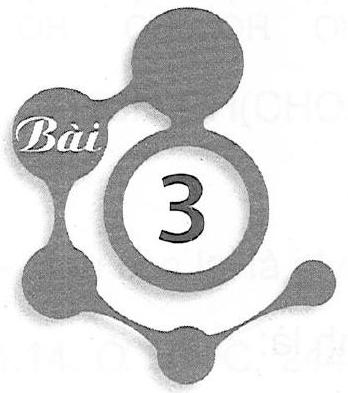
\includegraphics[max width=\textwidth]{2025_10_23_b4e16b74380d0f7e7700g-024}
\end{center}

\section*{GLUCOSE VÀ FRUCTOSE}
3.1. Đáp án $B$.\\
3.3. Đáp án C .\\
3.2. Đáp án D .\\
3.4. Đáp án D.\\
3.5. Đáp án C . Các phát biểu đúng là (2), (3) và (4).\\
3.6. Đáp án C .\\
3.8. Đáp án B.\\
3.7. Đáp án B.\\
3.9. Đáp án C.\\
3.10. Với glucose, ta có $1 \mathrm{mmol} / \mathrm{L}=180 \mathrm{mg} / \mathrm{L}=18 \mathrm{mg} / \mathrm{dL}$ nên đồ thị đã cho có thể biểu diễn lại theo $\mathrm{mg} / \mathrm{dL}$ như sau:\\
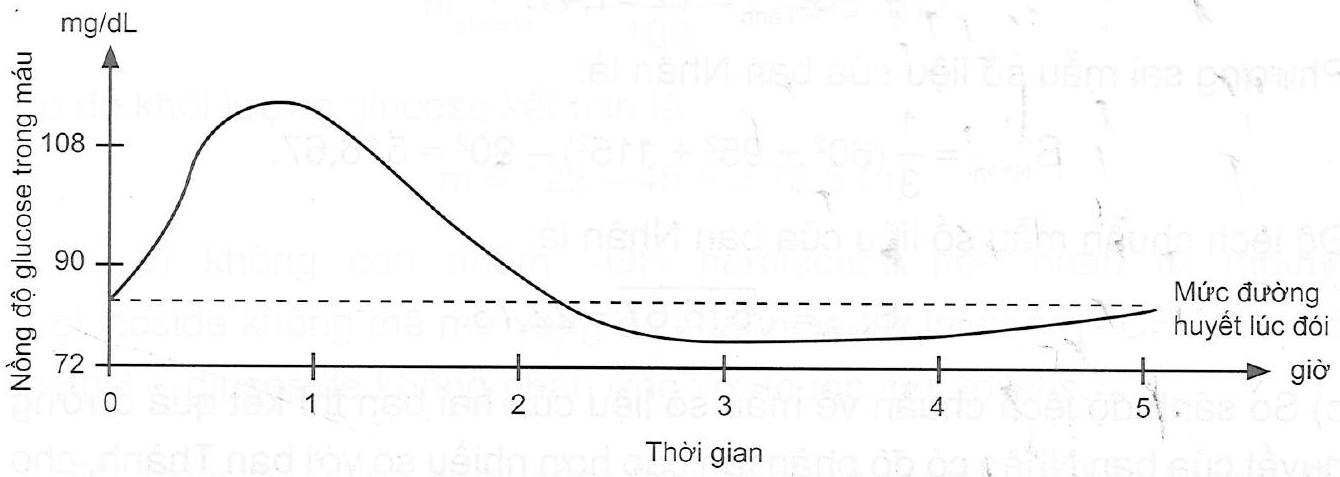
\includegraphics[max width=\textwidth, center]{2025_10_23_b4e16b74380d0f7e7700g-024(1)}

Trên đồ thị, chỉ số đường huyết lúc đói của người này khoảng $83 \mathrm{mg} / \mathrm{dL}$, đạt dưới $100 \mathrm{mg} / \mathrm{dL}$ nên có tình trạng đường huyết của người bình thường. Ngoài ra, sau khi thử nghiệm dung nạp glucose được 2 giờ, người này có đường huyết khoảng $90 \mathrm{mg} / \mathrm{dL}$, đạt dưới $140 \mathrm{mg} / \mathrm{dL}$, cho thấy đây là người khoẻ mạnh, không có dấu hiệu liên quan đến bệnh đái tháo đường.

Lưu ý: Nếu một người có chỉ số đường huyết dưới $70 \mathrm{mg} / \mathrm{dL}$ (tương đương khoảng $3,9 \mathrm{mmol} / \mathrm{L}$ ) được đánh giá là hạ đường huyết.\\
3.11. Xem nước là dung dịch glucose $0 \%$. Áp dụng sơ đồ đường chéo, ta có:\\
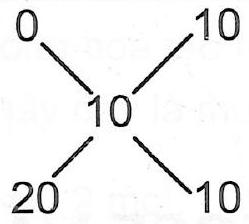
\includegraphics[max width=\textwidth, center]{2025_10_23_b4e16b74380d0f7e7700g-025}

Vậy $m_{\text {nước }}=m_{\text {dung dich glucose } 20 \%}=4 \mathrm{~g}$.\\
3.12. a) Chỉ số đường huyết trung bình của bạn Thành là:

$$
\frac{80+80+83}{3}=81(\mathrm{mg} / \mathrm{dL}) .
$$

Chỉ số đường huyết trung bình của bạn Nhân là:

$$
\frac{60+95+115}{3}=90(\mathrm{mg} / \mathrm{dL}) .
$$

b) Phương sai mẫu số liệu của bạn Thành là:

$$
S_{\text {Thành }}^{2}=\frac{1}{3}\left(80^{2}+80^{2}+83^{2}\right)-81^{2}=2 .
$$

Độ lệch chuẩn mẫu số liệu của bạn Thành là:

$$
S_{\text {Thành }}=\sqrt{2}=1,41 \text {. }
$$

Phương sai mẫu số liệu của bạn Nhân là:

$$
S_{\text {Nhân }}^{2}=\frac{1}{3}\left(60^{2}+95^{2}+115^{2}\right)-90^{2}=516,67 .
$$

Độ lệch chuẩn mẫu số liệu của bạn Nhân là:

$$
S_{\text {Nhän }}=\sqrt{516,67}=22,73 .
$$

c) So sánh độ lệch chuẩn về mẫu số liệu của hai bạn thì kết quả đường huyết của bạn Nhân có độ phân tán cao hơn nhiều so với bạn Thành, cho thấy đường huyết của bạn Thành trong tuần ổn định hơn, tức tốt hơn so với bạn Nhân.\\
3.13. Lần lượt trích một ít dung dịch ở các lọ làm mẫu thử.

\begin{itemize}
  \item Mẫu thử làm mất màu nước bromine là glucose:
\end{itemize}

$$
\mathrm{CH}_{2} \mathrm{OH}(\mathrm{CHOH})_{4} \mathrm{CHO}+\mathrm{Br}_{2}+\mathrm{H}_{2} \mathrm{O} \longrightarrow \mathrm{CH}_{2} \mathrm{OH}(\mathrm{CHOH})_{4} \mathrm{COOH}+2 \mathrm{HBr}
$$

\begin{itemize}
  \item Mẫu thử cho phản ứng tráng bạc là fructose:\\
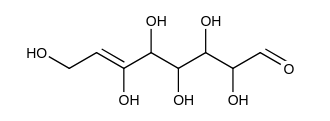
\includegraphics{smile-effaf37220136a48aae70f6025575b87cb7c37db}
\end{itemize}

$$
\begin{aligned}
& \mathrm{CH}_{2} \mathrm{OH}(\mathrm{CHOH})_{4} \mathrm{CHO}+2\left[\mathrm{Ag}\left(\mathrm{NH}_{3}\right)_{2}\right] \mathrm{OH} \xrightarrow{\mathrm{t}^{\circ}} \\
& \mathrm{CH}_{2} \mathrm{OH}(\mathrm{CHOH})_{4} \mathrm{COONH}_{4}+2 \mathrm{Ag}+3 \mathrm{NH}_{3}+\mathrm{H}_{2} \mathrm{O}
\end{aligned}
$$

\begin{itemize}
  \item Mẫu còn lại là glycerol.\\
3.14. Ơ $50^{\circ} \mathrm{C}, 244$ gam glucose tan được tối đa trong 100 g nước tạo 344 gam dung dịch. Khối lượng glucose và nước trong 172 g dung dịch glucose bão hoà ở $50^{\circ} \mathrm{C}$ là:
\end{itemize}

$$
\begin{gathered}
m_{\text {glucose }}=\frac{172 \times 244}{344}=122(\mathrm{~g}) \\
m_{\text {nước }}=172-122=50(\mathrm{~g})
\end{gathered}
$$

Ở $25^{\circ} \mathrm{C}, 100 \mathrm{~g}$ nước hoà tan được tối đa 91 g glucose nên 50 g nước sẽ hoà tan được một lượng tối đa glucose là:

$$
m_{\text {glucose }}=\frac{50 \times 91}{100}=45,5(\mathrm{~g}) .
$$

Do đó khối lượng glucose kết tinh là:

$$
m=122-45,5=76,5(g)
$$

3.15. Vì không còn nhóm -OH hemiacetal nên phân tử methyl $\alpha$-glucoside không thể mở vòng để xuất hiện trở lại nhóm -CHO . Do đó methyl $\alpha$-glucoside không phản ứng với thuốc thử Tollens.\\
3.16*. Trong tự nhiên, $\beta$-glucose bền hơn $\alpha$-glucose. Độ bền tương đối của $\alpha$-glucose và $\beta$-glucose xấp xỉ theo tỉ lệ $36: 64$.

Trong cấu tạo vòng của glucose, $\alpha$-glucose có nhóm 1-hydroxyl và 4-hydroxyl ở cùng phía, còn $\beta$-glucose có nhóm 1-hydroxyl và 4-hydroxyl ở các phía đối nhau. Chính điều đó đã làm cho $\alpha$-glucose bị cản trở lập thể bởi các nhóm -OH ở cùng phía nên $\alpha$-glucose sẽ kém bền hơn so với $\beta$-glucose.\\
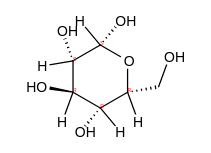
\includegraphics{smile-4f6b21af8319e07f12f90e78017b8a4370e942b2}

$\alpha$-glucose\\
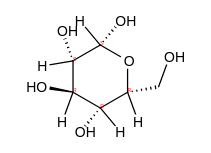
\includegraphics{smile-be3ae122e619128d74933506b2110e6297e4ba32}

$\beta$-glucose\\
3.17. Trong biểu đồ biểu diễn lượng đường huyết trước, trong và sau quá trình tập thể dục của một người khoẻ mạnh, không mắc bệnh tiểu đường cho thấy:

\begin{itemize}
  \item Quá trình tập thể dục diễn ra trong khoảng 70 phút.
  \item Lượng đường huyết giảm khi bắt đầu tập thể dục và xuống mức thấp nhất sau khi tập 20 phút, tăng lên mức cao nhất sau khi tập thể dục được 55 phút (xem ghi chú ở biểu đồ bên dưới).
  \item Sau khi dừng tập thể dục, lượng đường huyết có xu hướng giảm.
\end{itemize}

Vậy cả 4 phát biểu đã nêu đều đúng.\\
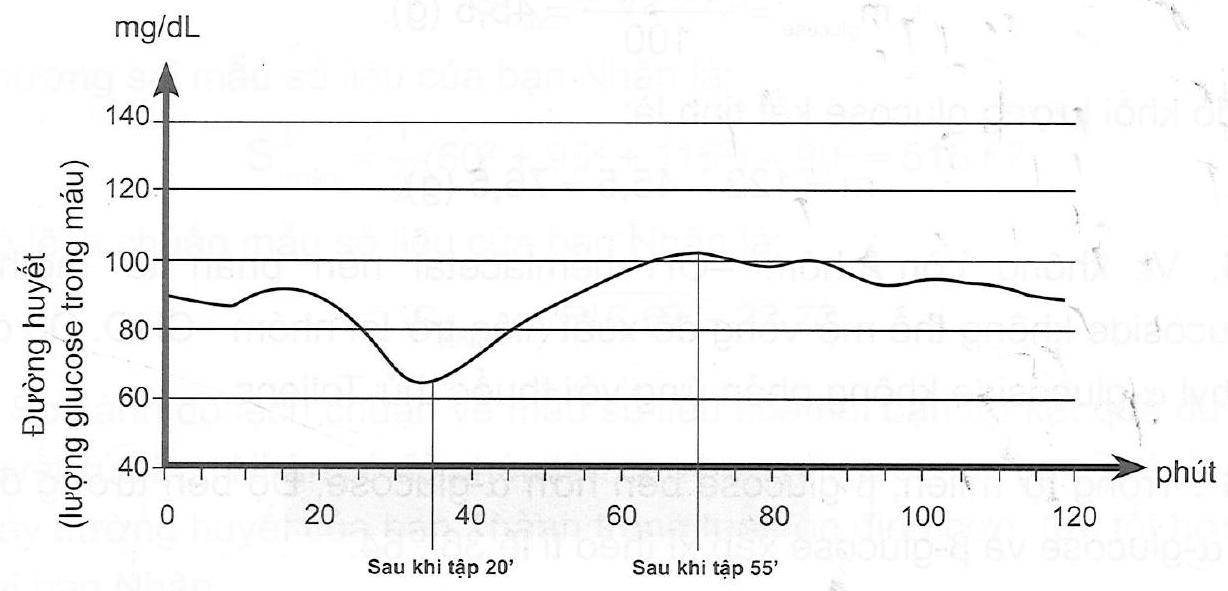
\includegraphics[max width=\textwidth, center]{2025_10_23_b4e16b74380d0f7e7700g-027}\\
3.18. Khi tập thể dục, việc sử dụng cơ bắp giúp đốt cháy glucose. Đó là lí do tại sao lượng đường huyết thường giảm trong giai đoạn đầu và sau khi kết thúc hoạt động.

Tuy nhiên, nếu việc luyện tập diễn ra lâu hoặc với cường độ cao, lượng đường trong máu có thể tăng lên. Đó là do cơ thể lúc này sản sinh hormone adrenaline giúp tăng lượng oxygen đến não và các cơ.

Adrenaline sẽ làm tăng nồng độ glucose trong máu bằng cách kích thích gan giải phóng glucose, dẫn đến lượng đường huyết tăng lên.\\
3.19*. Phương trình hoá học của phản ứng:\\
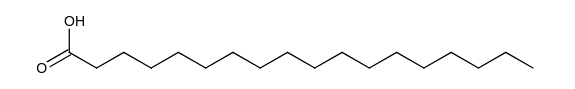
\includegraphics{smile-0881356f05c4158c3ec0f2dc5af676ad6bf03d05}

stearic acid\\
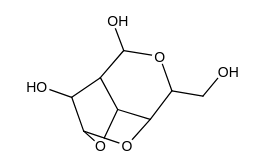
\includegraphics{smile-e6f83f2daa00e9a27b89bd1c91394c15d3e29aab}

$\beta$-glucose\\
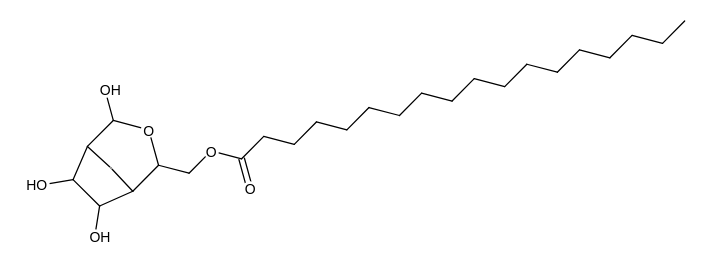
\includegraphics{smile-3fdd8a5eeb1e9f07e68882691b24ff372834fdca}

glucose monostearate\\
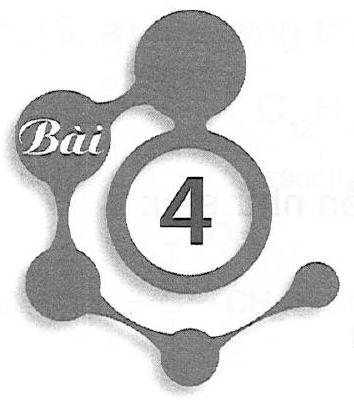
\includegraphics[max width=\textwidth, center]{2025_10_23_b4e16b74380d0f7e7700g-028}

\section*{SACCHAROSE VÀ MALTOSE}
4.1. Đáp án $B$.\\
4.3. Đáp án $A$.\\
4.5. Đáp án $C$.\\
4.6. Đáp án $C$.\\
4.2. Đáp án $A$.\\
4.4. Đáp án $C$.

Glucose, fructose và maltose có khả năng mở vòng để xuất hiện trở lại các nhóm aldehyde hoặc ketone.\\
4.7. Đáp án D .\\
4.8. Đáp án B.

Phương trình hoá học của phản ứng:

$$
\mathrm{C}_{12} \mathrm{H}_{22} \mathrm{O}_{11}+\mathrm{H}_{2} \mathrm{O} \xrightarrow{\mathrm{H}^{+}, \mathrm{t}^{\circ}} \mathrm{C}_{6} \mathrm{H}_{12} \mathrm{O}_{6}+\mathrm{C}_{6} \mathrm{H}_{12} \mathrm{O}_{6}
$$

Cứ a mol saccharose bị thuỷ phân sẽ tạo a mol gluocose và a mol fructose nên:

$$
\begin{aligned}
& 180 a+180 a+(100-342 a)=103,6 \\
& \Rightarrow a=0,2(\mathrm{~mol}) .
\end{aligned}
$$

Vậy hiệu suất phản ứng là:

$$
H=\frac{0,2 \times 342 \times 100 \%}{100}=68,4 \% .
$$

4.9. Đáp án C.

Phương trình hoá học của phản ứng:

$$
\begin{aligned}
\mathrm{C}_{12} \mathrm{H}_{22} \mathrm{O}_{11}+\mathrm{H}_{2} \mathrm{O} & \xrightarrow{\mathrm{H}^{+}, \mathrm{t}^{\circ}} 2 \mathrm{C}_{6} \mathrm{H}_{12} \mathrm{O}_{6} \\
342 \mathrm{~g} & \longrightarrow 2 \times 180 \mathrm{~g} \\
57 \mathrm{~g} & \longrightarrow \frac{57 \times 2 \times 180}{342}=60 \mathrm{~g}
\end{aligned}
$$

Vậy hiệu suất phản ứng là:

$$
H=\frac{57 \times 100 \%}{60}=95 \%
$$

4.10. Cấu trúc phân tử của saccharose được biểu diễn như sau:

\begin{figure}[h]
\begin{center}
  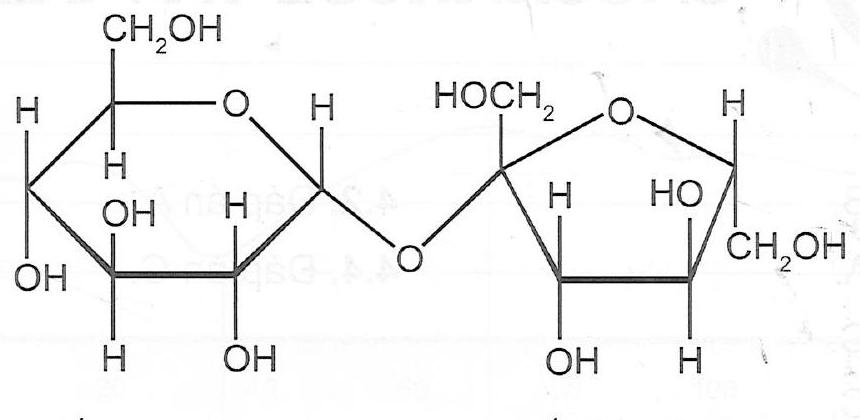
\includegraphics[width=\textwidth]{2025_10_23_b4e16b74380d0f7e7700g-029}
\captionsetup{labelformat=empty}
\caption{gốc $\alpha$-glucose gốc $\beta$-fructose}
\end{center}
\end{figure}

Trong cấu trúc này, nhóm -OH hemiacetal trên gốc $\alpha$-glucose và nhóm -OH hemiketal trên gốc $\beta$-fructose đều không còn hiện diện, do đó không vòng nào có thể mở để xuất hiện các nhóm aldehyde ( -CHO ) hoặc ketone (-CO-). Vì thế saccharose chỉ tồn tại một kiểu cấu trúc phân tử ở trạng thái rắn hoặc trong dung dịch.\\
4.11. Đường khử là thuật ngữ để chỉ các carbohydrate đóng vai trò chất khử do phân tử có sự hiện diện các nhóm aldehyde (- CHO ) hoặc nhóm ketone (-CO-). Carbohydrate không có nhóm aldehyde hoặc nhóm ketone thì không được gọi là đường khử.

Ở dạng mạch vòng, glucose, fructose và maltose không có sự hiện diện các nhóm chức trên, nhưng khi mở vòng thì xuất hiện trở lại các nhóm chức đã nêu làm chúng có khả năng đóng vai trò chất khử nên được gọi là đường khử.

Saccharose không phải là đường khử do saccharose không thể mở vòng.\\
4.12. Maltose là đường khử do có thể mở vòng, xuất hiện trở lại nhóm chức aldehyde. Do đó maltose tác dụng được với $\mathrm{NaBH}_{4}$ tương tự như một aldehyde. Saccharose không thể mở vòng để xuất hiện trở lại các nhóm aldehyde hoặc nhóm ketone, do đó saccharose không phản ứng được với $\mathrm{NaBH}_{4}$.\\
4.13. a) Phương trình hoá học của các phản ứng:\\
\includegraphics[max width=\textwidth, center]{2025_10_23_b4e16b74380d0f7e7700g-030}\\
\includegraphics[max width=\textwidth, center]{2025_10_23_b4e16b74380d0f7e7700g-030(1)}\\
b) Trong quá trình chế biến mứt, đường nghịch chuyển được hình thành vì có sự hỗ trợ bởi xúc tác là acid có trong trái cây và nhiệt độ khi đun nóng. Thợ làm mứt chuyên nghiệp sử dụng tính chất này để tăng hương vị của mứt vì đường nghịch chuyển giúp tạo độ mịn và.cảm giác ngon miệng hơn.\\
c) Phương trình hoá học của phản ứng:

$$
\mathrm{C}_{12} \mathrm{H}_{22} \mathrm{O}_{11}+\mathrm{H}_{2} \mathrm{O} \xrightarrow{\mathrm{H}^{+}, \mathrm{t}^{\circ}} \mathrm{C}_{6} \mathrm{H}_{12} \mathrm{O}_{6}+\mathrm{C}_{6} \mathrm{H}_{12} \mathrm{O}_{6}
$$

Cứ 342 g saccharose cần 18 g nước, nên 10 tấn saccharose cần:

$$
m_{\text {nước }}=\frac{10 \times 18}{342}=0,527 \text { (tấn). }
$$

Áp dụng định luật bảo toàn khối lượng, ta có:

$$
\begin{aligned}
m_{\text {đường nghich chuyền (max) }} & =m_{\text {glucose, fructose }}=m_{\text {saccharose }}+m_{\text {nước }} \\
& =10+0,527=10,527 \text { (tấn). }
\end{aligned}
$$

4.14. a) Do độ ngọt của đường nghịch chuyển cao hơn khoảng $20 \%$ $25 \%$ so với đường saccharose nên dùng đường nghịch chuyển trong pha chế thực phẩm giúp tiết kiệm chi phí hơn so với dùng đường saccharose.\\
b) Học sinh tiến hành thí nghiệm và hoàn thành báo cáo theo mẫu.\\
4.15*. a) Công thức phân tử của saccharose monolaurate là $\mathrm{C}_{24} \mathrm{H}_{44} \mathrm{O}_{12}$.\\
b) Saccharose monolaurate được sử dụng làm chất nhũ hoá do phân tử có một đầu ưa nước gắn với một đuôi dài kị nước.\\
\includegraphics[max width=\textwidth, center]{2025_10_23_b4e16b74380d0f7e7700g-031}\\
c) Saccharose monolaurate không phản ứng với thuốc thử Tollens do saccharose monolaurate không thể mở vòng.\\
d) Ta có $n_{\text {saccharose }}=\frac{500}{342}=1,46(\mathrm{~mol}) ; n_{\text {lauric acid }}=\frac{100}{200}=0,5(\mathrm{~mol})$.

Chú ý saccharose đã dùng dư, ta có phương trình hoá học của phản ứng:

$$
\begin{aligned}
& \mathrm{C}_{12} \mathrm{H}_{14} \mathrm{O}_{3}(\mathrm{OH})_{8}+\mathrm{C}_{11} \mathrm{H}_{23} \mathrm{COOH} \stackrel{\mathrm{H}^{+}, \mathrm{t}^{\circ}}{\rightleftharpoons} \mathrm{C}_{11} \mathrm{H}_{23} \mathrm{COOC}_{12} \mathrm{H}_{14} \mathrm{O}_{3}(\mathrm{OH})_{7}+\mathrm{H}_{2} \mathrm{O} \\
& 0,5(\mathrm{~mol}) \quad 0,5(\mathrm{~mol})
\end{aligned}
$$

Vậy khối lượng saccharose monolaurate thực tế thu được là:

$$
m=524 \times 0,5 \times 47 \%=123,14(g)
$$

4.16. Glucose là dạng đường đơn giản nhất, cơ thể có thể sử dụng ngay khi đi vào máu mà không cần trải qua bất kì quá trình trao đổi chất nào.

Do được tạo thành từ glucose và fructose, saccharose là một loại đường phức tạp hơn glucose. Cơ thể cần thuỷ phân saccharose trước khi có thể sử dụng làm năng lượng. Vì thế, glucose được dùng để truyền tĩnh mạch trong y học.\\
4.17*. a) Khi được thêm vào thực phẩm, đường liên kết với nước trong thực phẩm và tế bào vi sinh vật làm giảm lượng nước có sẵn cho sự phát triển của vi sinh vật, tương tự như hiện tượng thẩm thấu khi dùng nước muối trong sát trùng. Do vậy, khi cho thực phẩm vào dung dịch đường đậm đặc, nước sẽ bị hút ra khỏi tế bào của thực phẩm và vi sinh vật làm cho vi sinh vật không thể tồn tại được nữa.\\
b) Tuy nhiên, người ta thường sử dụng saccharose mà không phải glucose trong bảo quản do glucose khi mở vòng xuất hiện nhóm aldehyde dễ bị oxi hoá bởi các tác nhân xung quanh, trong khi saccharose không thể mở vòng nên không dễ bị oxi hoá.

\section*{5}
\section*{TINH BỘT VÀ CELLULOSE}
5.1. Đáp án $A$.\\
5.2. Đáp án B.\\
5.3. Đáp án $A$.\\
5.4. Đáp án A.

Tinh bột dạng amylopectin còn có thêm liên kết $\alpha-1,6$-glycoside.\\
5.5. Đáp án D.\\
5.6. Đáp án B.\\
5.7. Đáp án C.

Monosaccharide không cho được phản ứng thuỷ phân.\\
5.8. Đáp án C.\\
5.9. Đáp án D.\\
5.10. a) Tinh bột là thực phẩm chính trong bữa ăn hằng ngày ở nhiều nước trên thế giới. Sản phẩm của sự thuỷ phân tinh bột là glưcose đi trực tiếp vào máu qua đường tiêu hoá. Tuy nhiên, có một lượng lớn năng lượng được tạo thành từ tinh bột nên việc lạm dụng tinh bột có thể dẫn đến một số bệnh như béo phì và đái tháo đường, ...

Tinh bột kháng do không bị thuỷ phân thành glucose ở ruột non mà lên men trong ruột già nên tạo ra ít năng lượng hơn so với tinh bột bình thường, giúp hạn chế tình trạng béo phì và ổn định lượng đường huyết, hạn chế bệnh đái tháo đường. Bên cạnh đó, tinh bột kháng côn giúp ruột kết(*) khoẻ mạnh nhờ các vi khuẩn tốt trong ruột già có tác dụng biến tinh bột kháng thành các acid béo chuỗi ngắn. Đây là nguồn năng lượng "ưa thích" của các tế bào ruột kết.

Tinh bột kháng còn có vai trò như là một thành phần của chất xơ. Sự đa dạng chất xơ trong chế độ ăn uống là rất cần thiết do chúng hoạt động theo những cách khác nhau. Các chất xơ thường hiệu quả hơn khi kết hợp với nhau để duy trì một đường ruột khoẻ mạnh.

\footnotetext{(") Ruột kết còn gọi là đại trực tràng, phần dài nhất của ruột già và phần thấp nhất của hệ tiêu hoá.
}
b) Do tinh bột kháng có trong một số thực phẩm được nấu chín và để nguội, nhất là qua đêm như khoai tây, mì ống, cơm, ... nên cách đơn giản nhất để tăng lượng tinh bột kháng trong khẩu phần ăn hằng ngày là để nguội các thực phẩm chứa tinh bột như trên trong tủ lạnh qua đêm. Việc nấu và làm nguội lặp đi lặp lại sẽ làm tăng lượng tinh bột kháng trong các loại thực phẩm nói trên. Ngoài ra chuối xanh cũng là một nguồn tinh bột kháng đơn giản, dễ tìm.\\
5.11. Để hình thành phân tử cellulose, nhóm -OH ở vị trí nguyên tử carbon số 1 của đơn vị $\beta$-glucose này phản ứng với nhóm -OH ở vị trí nguyên tử carbon số 4 của đơn vị $\beta$-glucose kia hình thành nên các liên kết $\beta-1,4-$ glycoside trong phân tử cellulose như sau:\\
\includegraphics[max width=\textwidth, center]{2025_10_23_b4e16b74380d0f7e7700g-034(1)}\\
\includegraphics[max width=\textwidth, center]{2025_10_23_b4e16b74380d0f7e7700g-034}

Cách biểu diễn cấu trúc phân tử cellulose của bạn Nhân thể hiện được liên kết $\beta-1,4-$ glycoside nên đây là cách biểu diễn đúng. Bạn Thành biểu diễn sai do thể hiện liên kết $\alpha-1,4-$ glycoside không phù hợp với cấu trúc phân tử cellulose.\\
5.12. a) Phương trình hoá học của các phản ứng:

$$
\begin{aligned}
& \left(\mathrm{C}_{6} \mathrm{H}_{10} \mathrm{O}_{5}\right)_{n}+\mathrm{nH}_{2} \mathrm{O} \xrightarrow{\text { enzyme }} \mathrm{nC}_{6} \mathrm{H}_{12} \mathrm{O}_{6} \\
& \mathrm{C}_{6} \mathrm{H}_{12} \mathrm{O}_{6} \xrightarrow{\text { enzyme }} 2 \mathrm{C}_{2} \mathrm{H}_{5} \mathrm{OH}+2 \mathrm{CO}_{2}
\end{aligned}
$$

b) Theo phương trình, cứ 162 g cellulose thu được 92 g ethanol.

Vậy khối lượng ethanol thu được từ 1 tấn cellulose là:

$$
m_{\text {ethanol }}=\frac{1000 \times 92}{162} \approx 568(\mathrm{~kg})
$$

Do đó hiệu suất của quá trình điều chế là:

$$
H=\frac{240 \times 0,79}{568} \times 100 \% \approx 33,39 \%
$$

c) Do được 240 lít ethanol thì hiệu suất quá trình đạt $33,38 \%$.

Nên được 400 lít ethanol thì hiệu suất quá trình đạt

$$
H=\frac{400 \times 33,39 \%}{240} \times 100 \% \approx 55,65 \%
$$

5.13. Trong quá trình thực hiện bánh mì, khí carbon dioxide làm cho bột bánh mì nở ra và "dậy lên". Sau một thời gian, bột được nhào nặn để phá vỡ các bong bóng carbon dioxide này. Khi bánh mi được nướng, hơi nóng sẽ làm nở carbon dioxide giúp cho bánh mì nở ra nhiều hơn. Cuối cùng, nhiệt sẽ loại bỏ carbon dioxide cũng như ethanol và phần lớn nước được sử dụng để trộn bột, kết quả thu được bánh mì mềm, nhẹ và xốp.\\
5.14. Cộng sinh là mối quan hệ lâu dài, mật thiết giữa các sinh vật thuộc hai loài khác biệt. Sự cộng sinh giữa mối và vi sinh vật, cụ thể là Trichonympha sống trong ruột mối rất có lợi cho cả hai bên. Trichonympha tiết ra enzyme là cellulase giúp vật chủ là mối tiêu hoá cellulose, đổi lại Trichonympha nhận được môi trường bảo vệ cũng như nguồn cung cấp thức ăn liên tục.\\
5.15. Động vật nhai lại có thể tiêu hoá cellulose vì chúng có vi khuẩn Ruminococcus trong dạ cỏ tạo ra cellulase là enzyme có thể thuỷ phân cellulose thành glucose. Con người không thể sử dụng cellulose như một loại thực phẩm chính vì không có cellulase xúc tác cho phản ứng thuỷ phân cellulose thành glucose.\\
5.16. Tuy cellulose là một loại chất xơ không thể tiêu hoá được trong ruột của con người nhưng lại là thành phần quan trọng của một chế độ ăn uống lành mạnh, do chất xơ hỗ trợ sự hoạt động trơn tru của\\
đường ruột, giúp phòng tránh các bệnh về đường ruột như khó tiêu, trĩ, táo bón, ... Ngoài ra, chất xơ còn giúp giảm nguy cơ ung thư ruột kết do giảm thời gian phân tồn tại trong ruột kết.\\
5.17. Cấu trúc xoắn của phân tử amylose giúp cho các phân tử iodine có thể trượt vào trong vòng xoắn. Trong khi đó, cellulose có cấu trúc mạch thả̉ng, không phân nhánh nên phân tử cellulose không thể chứa các phân tử iodine như tinh bột. Vì vậy tinh bột cho được phản ứng màu với iodine còn cellulose không cho phản ứng này.\\
5.18. Tuy mỗi phân tử tinh bột có 1 nhóm -OH hemiacetal có thể mở vòng tạo nhóm aldehyde, chẳng hạn như hình dưới đây:

\begin{figure}[h]
\begin{center}
  \includegraphics[width=\textwidth]{2025_10_23_b4e16b74380d0f7e7700g-036(1)}
\captionsetup{labelformat=empty}
\caption{Mở vòng}
\end{center}
\end{figure}

\begin{center}
\includegraphics[max width=\textwidth]{2025_10_23_b4e16b74380d0f7e7700g-036}
\end{center}

Nhưng thực tế, tinh bột không phản ứng với thuốc thử Tollens. Điều này có thể giải thích là do trong hàng ngàn đơn vị saccharide tạo nên phân tử tinh bột, chỉ có 1 nhóm -OH hemiacetal ở đầu cuối, không đủ để kích hoạt phản ứng với thuốc thử Tollens.\\
5.19. a) Tuỳ thuộc vào số nhóm -OH trong mắt xích phân tử tinh bột đã bị nitrate hoá, phản ứng có thể tạo ra các sản phẩm khác nhau là $\left[\mathrm{C}_{6} \mathrm{H}_{7} \mathrm{O}_{2}(\mathrm{OH})_{2}\left(\mathrm{ONO}_{2}\right)\right]_{n},\left[\mathrm{C}_{6} \mathrm{H}_{7} \mathrm{O}_{2}(\mathrm{OH})\left(\mathrm{ONO}_{2}\right)_{2}\right]_{n}$ và $\left[\mathrm{C}_{6} \mathrm{H}_{7} \mathrm{O}_{2}\left(\mathrm{ONO}_{2}\right)_{3}\right]_{n}$.

Phương trình hoá học của các phản ứng:

$$
\begin{aligned}
& {\left[\mathrm{C}_{6} \mathrm{H}_{7} \mathrm{O}_{2}(\mathrm{OH})_{3}\right]_{n}+\mathrm{nHONO}_{2} \xrightarrow[60-70^{\circ} \mathrm{C}]{\mathrm{H}_{2} \mathrm{SO}_{4}}\left[\mathrm{C}_{6} \mathrm{H}_{7} \mathrm{O}_{2}(\mathrm{OH})_{2}\left(\mathrm{ONO}_{2}\right)\right]_{n}+\mathrm{nH}_{2} \mathrm{O}} \\
& {\left[\mathrm{C}_{6} \mathrm{H}_{7} \mathrm{O}_{2}(\mathrm{OH})_{3}\right]_{n}+2 \mathrm{nHONO}_{2} \xrightarrow[60-70^{\circ} \mathrm{C}]{\mathrm{H}_{2} \mathrm{SO}_{4}}\left[\mathrm{C}_{6} \mathrm{H}_{7} \mathrm{O}_{2}(\mathrm{OH})\left(\mathrm{ONO}_{2}\right)_{2}\right]_{n}+2 \mathrm{nH}_{2} \mathrm{O}} \\
& {\left[\mathrm{C}_{6} \mathrm{H}_{7} \mathrm{O}_{2}(\mathrm{OH})_{3}\right]_{n}+3 \mathrm{nHONO}_{2} \xrightarrow[60-70^{\circ} \mathrm{C}]{\mathrm{H}_{2} \mathrm{SO}_{4}}\left[\mathrm{C}_{6} \mathrm{H}_{7} \mathrm{O}_{2}\left(\mathrm{ONO}_{2}\right)_{3}\right]_{n}+3 \mathrm{nH}_{2} \mathrm{O}}
\end{aligned}
$$

b) Giả sử mẫu starch nitrate trên có công thức $\left[\mathrm{C}_{6} \mathrm{H}_{7} \mathrm{O}_{2}(\mathrm{OH})_{x}\left(\mathrm{ONO}_{2}\right)_{3-x}\right]_{n}$ Ta có $\% N=\frac{14 \times(3-x) \times 100}{(297-45 x)}=14,14 \Leftrightarrow x=0$.

Vậy công thức của mẫu starch nitrate đã cho là $\left[\mathrm{C}_{6} \mathrm{H}_{7} \mathrm{O}_{2}\left(\mathrm{ONO}_{2}\right)_{3}\right]_{n}$.\\
5.20. Tinh bột hay carbohydrate nói chung trong chế độ ăn uống cung cấp glucose để cơ thể sử dụng tạo năng lượng. Lượng glucose dư thừa vượt quá mức cơ thể cần để tạo năng lượng sẽ được chuyển hoá thành glycogen, một dạng tinh bột động vật. Khi lượng glycogen vượt quá giới hạn cho phép, cơ thể sẽ thích nghi bằng cách chuyển hoá lượng glucose dư thừa thành chất béo và được lưu trữ trong các tế bào mỡ của cơ thể. Khi lượng mỡ thừa và tích tụ đạt đến một mức nhất định, chúng sẽ gây béo phì. Vì thế, khi lượng tinh bột tiêu thụ quá nhiều có thể dẫn đến tình trạng béo phì.

\section*{ÔN TÂP CHUONG 2}
OT2.1. Đáp án B.\\
OT2.4. Đáp án B.\\
OT2.7. Đáp án A.

OT2.2. Đáp án D.\\
OT2.5. Đáp án C.\\
OT2.8. Đáp án D.

OT2.3. Đáp án D.\\
OT2.6. Đáp án C.\\
OT2.9. Đáp án C.

OT2.10. Các phân tử glucose và maltose còn nhóm -OH hemiacetal, phân tử fructose còn nhóm -OH hemiketal nên 3 phân tử này đều có thể mở vòng, trong đó maltose chỉ mở được một vòng.\\
\includegraphics{smile-ade24bf49a121731ac8ea60c29d28fd1cfc54d9d}

$\alpha$-glucose

\begin{figure}[h]
\begin{center}
  \includegraphics[width=\textwidth]{2025_10_23_b4e16b74380d0f7e7700g-038}
\captionsetup{labelformat=empty}
\caption{maltose}
\end{center}
\end{figure}

\includegraphics{smile-8bdbafc2142c4c27a739a469cb9d9a72a9e5bd1c}

$\beta$-fructose

Phân tử glucose, maltose, fructose có các nhóm -OH hemiacetal hoặc hemiketal nên có thể mở vòng

Phân tử saccharose không còn nhóm -OH hemiacetal cũng như nhóm -OH hemiketal do hai nhóm này đã tham gia phản ứng tạo liên kết $\alpha-1, \beta-2-$ glycoside. Do đó phân tử saccharose không thể mở vòng.\\
\includegraphics[max width=\textwidth, center]{2025_10_23_b4e16b74380d0f7e7700g-038(1)}

Phân tử saccharose không còn nhóm -OH hemiacetal hoặc hemiketal nên không thể mở vòng\\
OT2.11. Liên kết giữa hai đơn vị monosaccharide qua cầu nối oxygen do sự loại đi 1 phân tử nước được gọi là liên kết glycoside.\\
Ví dụ: Liên kết giữa hai đơn vị monosaccharide là $\alpha$-glucose và $\beta$-fructose qua cầu nối oxygen tạo nên phân tử saccharose là liên kết glycoside.

OT2.12. Để xác định tên liên kết, cần xác định kiểu vòng ( $\alpha, \beta$ ) và vị trí nguyên tử carbon nơi mỗi đơn vị monosaccharide tham gia liên kết.\\
a)

liên kết $\beta$-1,4-glycoside\\
\includegraphics{smile-8480a29702ca044dd1c6b9824b1a6783d041f69d}\\
b)

liên kết $\alpha-1,2-$ glycoside\\
\includegraphics[max width=\textwidth, center]{2025_10_23_b4e16b74380d0f7e7700g-039(2)}\\
c)\\
\includegraphics[max width=\textwidth, center]{2025_10_23_b4e16b74380d0f7e7700g-039}\\
d)\\
\includegraphics[max width=\textwidth, center]{2025_10_23_b4e16b74380d0f7e7700g-039(1)}

OT2.13. Vì 1 mol glucose khi bị oxi hoá tạo $6 \mathrm{~mol} \mathrm{CO}_{2}$ nên thể tích $\mathrm{CO}_{2}$ thải ra là:

$$
\mathrm{V}_{\mathrm{CO}_{2}}=\frac{60 \times 6 \times 25,4}{180}=50,8 \text { (lit). }
$$

OT2.14. Từ phương trình nhiệt hoá học của các phản ứng đã cho, ta có: $2 \mathrm{CH}_{3} \mathrm{COOH}(\mathrm{l})+2 \mathrm{H}_{2} \mathrm{O}(\mathrm{l}) \longrightarrow 2 \mathrm{C}_{2} \mathrm{H}_{5} \mathrm{OH}(\mathrm{l})+2 \mathrm{O}_{2}(\mathrm{~g}) \Delta_{\mathrm{r}} \mathrm{H}_{298}^{0}=985,2 \mathrm{~kJ} 4 \mathrm{CO}_{2}(\mathrm{~g})+4 \mathrm{H}_{2} \mathrm{O}(\mathrm{l}) \longrightarrow 2 \mathrm{CH}_{3} \mathrm{COOH}(\mathrm{l})+4 \mathrm{O}_{2}(\mathrm{~g}) \quad \Delta_{\mathrm{r}} \mathrm{H}_{298}^{\circ}=1748,4 \mathrm{~kJ} \mathrm{C}_{6} \mathrm{H}_{12} \mathrm{O}_{6}(\mathrm{~s})+6 \mathrm{O}_{2}(\mathrm{~g}) \longrightarrow 6 \mathrm{CO}_{2}(\mathrm{~g})+6 \mathrm{H}_{2} \mathrm{O}(\mathrm{l}) \quad \Delta_{\mathrm{r}} \mathrm{H}_{298}^{\circ}=-2805,0 \mathrm{~kJ}$\\
Cộng 3 phản ứng trên, kết quả có được là:\\
\includegraphics[max width=\textwidth, center]{2025_10_23_b4e16b74380d0f7e7700g-040}

OT2.15*. a) Cấu trúc phân tử của $\beta$-glucose và $\beta$-galactose khác nhau ở nguyên tử carbon số 4:\\
\includegraphics{smile-6278cdebffc6783a5af43cbb1f475e2092f311a7}

$\beta$-glucose\\
\includegraphics{smile-867b903398adadf86290bd19be4fd81a169aed99}

$\beta$-galactose\\
b) Do còn nhóm -OH hemiacetal nên phân tử $\beta$-galactose có thể mở vòng, xuất hiện trở lại nhóm - CHO nên $\beta$-galactose phản ứng được với thuốc thử Tollens.

OT2.16*. a) Khi có thể có quá ít lactase, một loại enzyme được sản xuất trong ruột non, thường là nguyên nhân gây ra tình trạng không dung nạp lactose. Một người có lượng lactase thấp vẫn có thể tiêu hoá được các sản phẩm từ sữa. Tuy nhiên mức độ lactase quá thấp dẫn đến cơ thể không dung nạp được một lượng lớn lactose, từ đó xuất hiện các triệu chứng sau khi dùng các sản phẩm từ sữa như đầy bụng, sình hơi, tiêu chảy, thậm chí có thể ói mửa.\\
b) Cấu trúc phân tử lactose:

\begin{figure}[h]
\begin{center}
  \includegraphics[width=\textwidth]{2025_10_23_b4e16b74380d0f7e7700g-041(1)}
\captionsetup{labelformat=empty}
\caption{Phân tử lactose}
\end{center}
\end{figure}

c) Do còn nhóm -OH hemiacetal, phân tử lactose có thể mở vòng, xuất hiện trở lại nhóm - CHO nên lactose phản ứng được với thuốc thử Tollens. Vậy lactose là đường khử.\\
OT2.17. Tinh bột tạo bởi các đơn vị $\alpha$-glucose, nối với nhau bởi liên kết $\alpha-1,4-$ glycoside, ngoài ra có thể có thêm liên kết $\alpha-1,6-$ glycoside. Trong khi cellulose tạo bởi các đơn vị $\beta$-glucose nối với nhau chỉ bởi liên kết $\beta-1,4-$ glycoside. Dịch tiêu hoá của con người thiếu nhữung enzyme có thể thuỷ phân các liên kết $\beta-1,4-$ glycoside trong cellulose. Do đó, con người không thể sử dụng cellulose làm thức ăn chính thay thế cho tinh bột.\\
Cellulase là một loại enzyme được sản xuất bởi một số động vật nguyên sinh cộng sinh (ví dụ như Trichonympha) trong ruột của động vật nhai lại và mối, có khả năng phá vỡ liên kết $\beta-1,4$-glycoside, do đó các loài này có thể sử dụng cellulose làm thức ăn chính.\\
OT2.18*. Công thức phân tử của saccharose monostearate là $\mathrm{C}_{30} \mathrm{H}_{56} \mathrm{O}_{12}$. OT2.19*. a) Cấu trúc hoá học của saccharose octaacetate (chú ý AcO là kí hiệu cho nhóm $\mathrm{CH}_{3} \mathrm{COO}$ ):\\
\includegraphics[max width=\textwidth, center]{2025_10_23_b4e16b74380d0f7e7700g-041}

Phương trình hoá học của phản ứng điều chế saccharose octaacetate từ saccharose và acetic anhydride với xúc tác sodium acetate:\\
\includegraphics[max width=\textwidth, center]{2025_10_23_b4e16b74380d0f7e7700g-042(1)}\\
\includegraphics[max width=\textwidth, center]{2025_10_23_b4e16b74380d0f7e7700g-042}\\
b) Ta có $n_{\text {saccharose }}=\frac{10}{342}=0,029(\mathrm{~mol}) ; n_{\left(\mathrm{CH}_{3} \mathrm{CO}\right)_{2} \mathrm{O}}=\frac{30 \times 1,08}{102}=0,317(\mathrm{~mol})$.

Do $\mathrm{n}_{\left(\mathrm{CH}_{3} \mathrm{CO}\right)_{2} \mathrm{O}}>8 \mathrm{n}_{\text {saccharose }}$ nên acetic anhydride đã dùng dư.\\
Vậy khối lượng saccharose octaacetate ( $\mathrm{C}_{28} \mathrm{H}_{38} \mathrm{O}_{19}$ ) thực tế thu được là:

$$
\mathrm{m}_{\mathrm{C}_{28} \mathrm{H}_{38} \mathrm{O}_{19}}=\frac{678 \times 0,029 \times 75}{100}=14,746(\mathrm{~g})
$$

c) "Hoá học xanh" là khái niệm về phát triển hoá học một cách bền vững, thông qua việc hạn chế sử dụng hoặc tạo thạ̀nh sản phẩm phụ là các hoá chất độc hại, tránh gây ô nhiễm môi trường. "Hoá học xanh" cũng hướng đến việc ngăn ngừa sự lãng phí như tránh phát sinh chất thải phải xử lí; sử dụng dung môi và điều kiện phản ứng an toàn; tăng hiệu quả sử dụng năng lượng như ưu tiên tiến hành phản ứng ở nhiệt độ và áp suất phòng khi có thể; ưu tiên tạo thành sản phẩm có khả năng phân huỷ thành các chất vô hại sau sử dụng, ...

Ví dụ: Trong tổng hợp saccharose octaacetate ở trên, xúc tác sodium acetate khi thải ra môi trường có khả năng ảnh hưởng đến hệ sinh thái dưới nước, do làm pH của nước vượt quá phạm vi cho phép. Khi tiếp xúc với da, sodium acetate có thể gây kích ứng với mẩn đỏ và đau ngứa, ... Tất cả những điều này sẽ được giải quyết nếu xúc tác sodium acetate được thay thế bằng sự chiếu xạ siêu âm. Đó là một trong những khía cạnh hoá học xanh mang lại trong tổng hợp saccharose octaacetate.

\begin{table}[h]
\begin{center}
\captionsetup{labelformat=empty}
\caption{OT2.20.}
\begin{tabular}{|l|l|l|}
\hline
Phát biểu & Đúng & Sai \\
\hline
a) Glucose là monosaccharide do glucose không cho được phản ứng thuỷ phân. & $\checkmark$ &  \\
\hline
b) Saccharose là disaccharide do thuỷ phân một phân tử saccharose thu được một phân tử glúcose và một phân tử fructose. & $\checkmark$ &  \\
\hline
c) Maltose là monosaccharide do thuỷ phân maltose chỉ thu được glucose. &  & $\checkmark$ \\
\hline
d) Cellulose là polysaccharide do thuỷ phân một phân tử cellulose thu được nhiều phân tử glucose. & $\checkmark$ &  \\
\hline
\end{tabular}
\end{center}
\end{table}

OT2.21.

\begin{center}
\begin{tabular}{|l|l|l|}
\hline
Phát biểu & Đúng & Sai \\
\hline
a) Phân tử saccharose không còn nhóm - OH hemiacetal và nhóm -OH hemiketal. & $\checkmark$ &  \\
\hline
b) Phân tử saccharose và maltose đều không có khả năng mở vòng. &  & $\checkmark$ \\
\hline
c) Phân tử saccharose tạo bởi một đơn vị $\beta$-glucose và một đơn vị $\alpha$-fructose, liên kết với nhau qua nguyên tử oxygen giữa $\mathrm{C}_{1}$ của đơn vị $\beta$-glucose và $\mathrm{C}_{4}$ của đơn vị $\alpha$-fructose. &  & $\checkmark$ \\
\hline
d) Saccharose và maltose đều là các disaccharide. & $\checkmark$ &  \\
\hline
\end{tabular}
\end{center}

\begin{table}[h]
\begin{center}
\captionsetup{labelformat=empty}
\caption{OT2.22.}
\begin{tabular}{|l|l|l|}
\hline
Phát biều & Đúng & Sai \\
\hline
a) Phân tử maltose tạo bởi hai đơn vị glucose, liên kết với nhau qua nguyên tử oxygen giữa $\mathrm{C}_{1}$ của đơn vị glucose này và $\mathrm{C}_{4}$ của đơn vị glucose kia. & $\checkmark$ &  \\
\hline
b) Phân tử maltose còn một nhóm - OH hemiacetal. & $\checkmark$ &  \\
\hline
c) Thuỷ phân maltose chỉ thu được glucose. & $\checkmark$ &  \\
\hline
d) Maltose không có khả năng phản ứng với thuốc thử Tollens. &  & $\checkmark$ \\
\hline
\end{tabular}
\end{center}
\end{table}

OT2.23.

\begin{center}
\begin{tabular}{|l|l|l|}
\hline
Phát biểu & Đúng & Sai \\
\hline
a) Phân tử amylose tạo bởi nhiều đơn vị $\beta$-glucose, nối với nhau qua liên kết $\beta-1,4-$ glycoside. &  & $\checkmark$ \\
\hline
b) Phân tử cellulose tạo bởi nhiều đơn vị $\alpha$-glucose, nối với nhau qua liên kết $\alpha-1,4-$ glycoside. &  & $\checkmark$ \\
\hline
c) Amylose và cellulose đều là những polymer mạch không phân nhánh. & $\checkmark$ &  \\
\hline
d) Thuỷ phân amylose hoặc cellulose đều thu được glucose. & $\checkmark$ &  \\
\hline
\end{tabular}
\end{center}

\begin{center}
\begin{tabular}{|c|c|c|c|c|c|c|}
\hline
Câu & OT1.24 & OT1.25 & OT1.26 & OT1.27 & OT1.28 & OT1.29 \\
\hline
Đáp án & 4 & 2 & 4,3 & 20 & 15,6 & 63,5 \\
\hline
\end{tabular}
\end{center}

OT2.24. Trong số 6 carbohydrate: glucose, fructose, saccharose, maltose, tinh bột và cellulose, có 4 carbohydrate cho được phản ứng thựy phân là saccharose, maltose, tinh bột và cellulose.\\
OT2.25. Trong số 4 carbohydrate: glucose, fructose, saccharose và maltose, có 2 carbohydrate có nhóm -OH hemiacetal trong phân tử là glucose và maltose.

OT2.26. Phương trình hoá học của phản ứng:

$$
\underset{\text { saccharose }}{\mathrm{C}_{12} \mathrm{H}_{22} \mathrm{O}_{11}}+\mathrm{H}_{2} \mathrm{O} \xrightarrow{\mathrm{H}^{+}, \mathrm{t}^{\circ}} \underset{\text { glucose }}{\mathrm{C}_{6} \mathrm{H}_{12} \mathrm{O}_{6}}+\underset{\text { fructose }}{\mathrm{C}_{6} \mathrm{H}_{12} \mathrm{O}_{6}}
$$

Cứ a mol saccharose bị thuỷ phân tạo a mol gluocose và a mol fructose nên:

$$
180 a+180 a+(10-342 a)=10,3 \Rightarrow a=\frac{1}{60}(m o l) .
$$

Vậy khối lượng saccharose còn dư là:

$$
m_{\text {saccharose du }}=10-342 a=10-342 \times \frac{1}{60}=4,3(g) .
$$

OT2.27. Theo đề, có $0,2 \mathrm{~mol} \mathrm{CO}_{2}$ sinh ra từ phản ứng lên men tinh bột:

$$
\left(\mathrm{C}_{6} \mathrm{H}_{10} \mathrm{O}_{5}\right)_{\mathrm{n}}+\mathrm{nH}_{2} \mathrm{O} \xrightarrow{\text { enzyme }} 2 \mathrm{nC}_{2} \mathrm{H}_{5} \mathrm{OH}+2 \mathrm{nCO}_{2}
$$

Vậy $m=\frac{0,2 \times 162 n \times 100}{2 n \times 81}=20(g)$.\\
OT2.28. Xem X có công thức $\mathrm{C}_{\mathrm{n}}\left(\mathrm{H}_{2} \mathrm{O}\right)_{\mathrm{m}}$ (a mol) thì khi đốt X thu được an $\mathrm{mol} \mathrm{CO}_{2}$ và am $\mathrm{mol} \mathrm{H}_{2} \mathrm{O}$.

Vậy khối lượng rắn X là:

$$
m_{x}=a(12 n+18 m)=12 \times 0,55+18 \times 0,5=15,6(g) .
$$

OT2.29. Số mol oxygen thu được là:

$$
n=\frac{P V}{R T}=\frac{(1-0,035) \times 0,06}{0,082 \times 300}=0,00235(\mathrm{~mol}) .
$$

Phương trình hoá học của phản ứng:

$$
6 \mathrm{nCO}_{2}+5 \mathrm{nH}_{2} \mathrm{O} \xrightarrow{\text { enzyme }}\left(\mathrm{C}_{6} \mathrm{H}_{10} \mathrm{O}_{5}\right)_{n}+6 \mathrm{nO}_{2}
$$

Vậy khối lượng tinh bột thu được là:

$$
m_{\text {tinh bột }}=\frac{0,00235 \times 162 \times 1000}{6}=63,5(\mathrm{mg}) .
$$

\section*{Chuong 3. HOP CHÁT CHÚA NHHROGEN}
\begin{center}
\includegraphics[max width=\textwidth]{2025_10_23_b4e16b74380d0f7e7700g-046}
\end{center}

\section*{AMINE}
6.1. Đáp án A .\\
6.2. Đáp án $C$.\\
6.3. Đáp án D.\\
6.4. Đáp án B.\\
6.5. Đáp án A.\\
6.6. Đáp án B.\\
6.7. Đáp án D.\\
6.8. Đáp án A.\\
6.9. Đáp án B.\\
6.10. Đáp án C.\\
6.11. Đáp án $A$.\\
6.12. Đáp án D.\\
6.13. Sự liên hợp của cặp electron chưa liên kết của nguyên tử nitrogen với hệ thống electron vòng benzene làm giảm mật độ electron của nguyên tự nitrogen, dẫn đến tính base của amine giảm.\\
6.14. a) Các chất có phân tử khối tương đương (lần lượt theo thứ tự là trimethylamine, $\mathrm{M}=59$; ethylmethylether, $\mathrm{M}=60$; ethylmethylamine, $\mathrm{M}=59$; propylamine, $\mathrm{M}=59$; propyl alcohol, $\mathrm{M}=60$ ) nhưng nhiệt độ sôi rất khác nhau, tăng dần từ trimethylamine (có nhiệt độ sôi nhỏ nhất, $3^{\circ} \mathrm{C}$ ) đến propyl alcohol (có nhiệt độ sôi lớn nhất, $97^{\circ} \mathrm{C}$ ).\\
b) So với 2 amine $\mathrm{CH}_{3} \mathrm{CH}_{2}-\mathrm{NH}-\mathrm{CH}_{3}$ và $\mathrm{CH}_{3} \mathrm{CH}_{2} \mathrm{CH}_{2}-\mathrm{NH}_{2}$ thì $\left(\mathrm{CH}_{3}\right)_{3} \mathrm{~N}$ không hình thành được liên kết hydrogen liên phân tử, dẫn đến nhiệt độ sôi của $\left(\mathrm{CH}_{3}\right)_{3} \mathrm{~N}$ sẽ nhỏ hơn.

Nhóm $-\mathrm{NH}_{2}$ của $\mathrm{CH}_{3} \mathrm{CH}_{2} \mathrm{CH}_{2} \mathrm{NH}_{2}$ có nhiều hydrogen linh động nên tạo được nhiều liên kết hydrogen hơn so với nhóm $-\mathrm{NH}-$ của $\mathrm{CH}_{3} \mathrm{CH}_{2} \mathrm{NHCH}_{3}$.

Nitrogen có độ âm điện $(3,04)$ nhỏ hơn oxygen $(3,44)$ nên nhóm $-\mathrm{NH}_{2}$ của $\mathrm{CH}_{3} \mathrm{CH}_{2} \mathrm{CH}_{2} \mathrm{NH}_{2}$ hình thành liên kết hydrogen kém bền hơn so với liên kết hydrogen được hình thành từ nhóm -OH của $\mathrm{CH}_{3} \mathrm{CH}_{2} \mathrm{CH}_{2} \mathrm{OH}$.\\
6.15. Dựa vào giản đồ năng lượng, arylamine có mức năng lượng thấp hơn alkylamine, nên khi proton hoá, arylamine cần năng lượng lớn hơn alkylamine, tính base của arylamine yếu hơn alkylamine.

Quá trình proton hoá 2 amine trên là quá trình thu nhiệt. Arylamine cần cung cấp nhiều năng lượng hơn so với alkylamine.\\
6.16. Butane-1,4-diamine (putrescine) và pentane-1,5-diamine (cadaverine) là diamine được tìm thấy trong thịt dần bị phân huỷ. Có thể sử dụng các biện pháp làm giảm hoặc khử mùi hôi, tuy nhiên loại thực phẩm này đã biến chất, không đảm bảo an toàn để chế biến.\\
6.17. Nguyên tử nitrogen của nhóm amine còn cặp electron chưa liên kết nên dễ hình thành liên kết cho - nhận với một số kim loại nhóm B (bán kính nguyên tử lớn, có orbital trống, ...). Đó là khả năng tạo phức chất của các amine.\\
6.18. Một số gợi ý:

Thuốc nhuộm được sử dụng rộng rãi trong đời sống con người để tạo ra màu sắc và hiệu ứng trên các vật liệu như vải, da, giấy và tóc. Dưới đây là một số lợi ích, hạn chế của thuốc nhuộm nói chung và thuốc nhuộm azo nói riêng đối với đời sống con người.

Lợi ích của thuốc nhuộm

\begin{itemize}
  \item Tạo màu sắc đa dạng: Thuốc nhuộm tạo ra nhiều màu sắc khác nhau trên các vật liệu, từ những sắc thái tươi sáng đến nhữung màu sắc đậm.
  \item Cải thiện thẩm mĩ: Thuốc nhuộm tạo ra những sản phẩm có màu sắc hấp dẫn và thu hút người tiêu dùng, cải thiện thẩm mĩ của sản phẩm như quần áo, nội thất hoặc sản phẩm trang điểm.
  \item Tăng cá tính: Thuốc nhuộm cho phép mỗi người tuỳ chỉnh màu sắc tóc, thời trang theo sở thích và phong cách cá nhân, giúp tạo nên sự độc đáo và cá nhân hoá.
  \item Bổ sung phụ liệu cho nhiều ngành công nghiệp: Ngành công nghiệp dệt may và sản xuất quần áo lớn phụ thuộc vào thuốc nhuộm để cung cấp những màu sắc và kiểu dáng khác nhau cho sản phẩm.
\end{itemize}

\section*{Hạn chế của thuốc nhuộm}
\begin{itemize}
  \item Tiềm ẩn nguy cơ sức khoẻ: Một số thuốc nhuộm, đặc biệt là thuốc nhuộm azo có thể gây nguy hiểm cho sức khoẻ nếu sử dụng không đúng cách. Nhiều thuốc nhuộm có thể gây kích ứng da, dị ứng hoặc tăng nguy cơ mắc bệnh ung thư.
  \item Gây ô nhiễm môi trường: Quá trình nhuộm màu có thể tạo ra các chất thải và chất độc có thể gây ô nhiễm môi trường nếu không xử lí đúng cách. Các hợp chất hoá học từ việc nhuộm màu có thể gây hại môi trường.\\
6.19. Một số gợi ý về vấn đề nên hay không nên ban hành luật cấm sản xuất và sử dụng thuốc nhuộm azo trong công nghiệp may mặc, dệt nhuộm.
\end{itemize}

\section*{Ủng hộ việc cấm}
\begin{itemize}
  \item Nguy cơ cho sức khoẻ: Thuốc nhuộm hoặc thuốc nhuộm azo chứa các hoá chất độc hại, có thể gây ra những bệnh nguy hiểm, bao gồm cả ung thư. Cấm sử dụng thuốc nhuộm azo giúp bảo vệ sức khoẻ người lao động (công nhân) và người tiêu dùng trong ngành công nghiệp may mặc và dệt nhuộm.
  \item Bảo vệ môi trường: Quá trình sản xuất và sử dụng thuốc nhuộm azo thường gây ra ô nhiễm môi trường nghiêm trọng. Việc cấm sử dụng thuốc nhuộm azo sẽ giúp giảm lượng chất thải độc hại được thải ra và bảo vệ môi trường.
  \item Thúc đẩy sử dụng thuốc nhuộm an toàn: Bằng cách cấm sử dụng thuốc nhuộm azo, cơ quan chức năng và ngành công nghiệp có thể tập trung vào phát triển và sử dụng các loại thuốc nhuộm an toàn hơn, không gây hại cho sức khoẻ và môi trường.
\end{itemize}

\section*{Không nên cấm}
\begin{itemize}
  \item Ảnh hưởng đến ngành công nghiệp: Cấm sử dụng thuốc nhuộm azo gây ảnh hưởng đáng kể đến ngành công nghiệp may mặc và dệt nhuộm. Điều này có thể gây mất việc làm và khó khăn cho các doanh nghiệp trong ngành.
  \item Khó thực hiện và kiểm soát: Kiểm soát và thực hiện việc cấm sử dụng thuốc nhuộm azo có thể gặp khó khắn do sự phức tạp của chuỗi cung ứng và khả năng giám sát của cơ quan chức năng.
  \item Cần thiết của sự thay thế: Có thể cần thời gian và nỗ lực để phát triển cũng như chuyển đổi sang các loại thuốc nhuộm thay thế an toàn.\\
6.20. Hiện trạng nưởc thải từ ngành công nghiệp dệt nhuộm vẫn đang gặp nhiều thách thức và ảnh hưởng tiêu cực đến môi trường.
  \item Ô nhiễm nước: Ngành công nghiệp dệt nhuộm tạo ra lượng lớn nước thải chứa hoá chất, chất phụ gia, ... Nước thải này thường có màu sắc, pH cao hoặc thấp và có thể chứa các chất độc hại như thuốc nhuộm, phenol, aniline, formaldehyde và các kim loại nặng. Khi nước thải này được thải ra môi trường mà không qua xử lí hoặc xử lí không triệt để sẽ gây ô nhiễm cho nguồn nước.
  \item Thiếu hệ thống xử lí nước thải hiệu quả: Một số doanh nghiệp trong ngành công nghiệp dệt nhuộm có thể chưa đủ quy mô, tài chính để đầu tư vào hệ thống xử lí nước thải hiệu quả. Điều này dẫn đến việc nước thải chưa được xử lí đúng cách trước khi được thải ra môi trường.
  \item Quy định và thực thi pháp luật: Mặc dù đã có quy định pháp luật về quản lí và xử lí nước thải công nghiệp, nhưng việc thực thi và kiểm soát vẫn còn hạn chế. Một số doanh nghiệp vẫn không tuân thủ đúng quy định và tiếp tục xả nước thải chưa qua xử lí vào môi trường.
  \item Nhận thức và tinh thần bảo vệ môi trường: Nhận thức về tác động của nước thải dệt nhuộm đối với môi trường và sức khoẻ cần được nâng cao. Cả doanh nghiệp và người tiêu dùng cần có trách nhiệm hơn,\\
khuyến khích việc sử dụng các quy trình nhuộm và công nghệ xanh hơn để giảm thiểu tác động tiêu cực đến môi trường.
\end{itemize}

Để cải thiện hiện trạng nước thải dệt nhuộm, cần có sự hợp tác giữa cơ quan chuyên trách, các doanh nghiệp và cộng đồng. Đầu tư vào công nghệ xử lí nước thải hiệu quả, tăng cường kiểm tra và kiểm soát tuân thủ quy định, tăng cường nhận thức về bảo vệ môi trường là những yếu tố quan trọng để giảm thiểu ô nhiễm nước từ ngành công nghiệp dệt nhuộm.

\section*{AMINO ACID VÀ PEPTIDE}
7.1. Đáp án B.\\
7.5. Đáp án A .\\
7.9. Đáp án B .\\
7.2. Đáp án C.\\
7.6. Đáp án $C$. 7.10. Đáp án C.\\
7.3. Đáp án A.\\
7.7. Đáp án D .\\
7.4. Đáp án D .\\
7.8. Đáp án A.\\
7.11. Cấu trúc ion lưỡng cực của phân tử alliin như sau:\\
\includegraphics{smile-808966edbd28a54bf94b551fffb1f2ba3d7d1397}\\
7.12. Tương tác chủ yếu giữa các phân tử chất béo (triester) thường là tương tác van der Waals, giữa các phân tử acid béo còn cở liên kết hydrogen, giữa các phân tử glycine là liên kết ion. Độ bền liên kết giữa các phân tử trong hợp chất tăng dần nên nhiệt độ nóng chảy tăng dần.\\
7.13. a) Tuỳ thuộc vào pH môi trường, mỗi amino acid cớ điểm đẳng điện khác nhau sẽ tồn tại dạng ion chủ yếu khác nhau, có thể anion, cation hoặc ion lưỡng cực. Các ion này có thể đứng yên hoặc di chuyển trong trường điện dựa vào tính chất điện di của amino acid.\\
b) Trong dung dịch có $\mathrm{pH}=6$, là môi trường acid mạnh đối với Lys, là môi trường base mạnh đối với Glu, là môi trường trung tính đối với Ala.

Vì vậy:

\begin{itemize}
  \item Ion tồn tại chủ yếu đối với Lys là cation, sẽ di chuyển về cực âm của nguồn điện nên vệt (1) là Lys*.
  \item Ion tồn tại chủ yếu đối với Ala là ion lưỡng cực, không di chuyển nên vệt (2) là Ala.
  \item Ion tồn tại chủ yếu đối với Glu là anion, sẽ di chuyển về cực dương của nguồn điện nên vệt (3) là Glu-.\\
7.14. a) Bradykinin được tạo thành từ 9 đơn vị amino acid, gọi là nonapeptide. Phân tử có 8 liên kết peptide. Các amino acid khác nhau tạo nên Bradykinin là arginine, proline, glycine, phenylalanine, serine.\\
b) Tên viết tắt của Bradykinin: Arg-Pro-Pro-Gly-Phe-Ser-Pro-Phe-Arg\\
7.15. Điểm đẳng điện của các amino acid được hoàn thành như sau:
\end{itemize}

\begin{center}
\begin{tabular}{|l|l|l|l|}
\hline
Amino acid & pK ${ }_{\mathrm{a}}$ của. $\alpha-\mathrm{COOH}$ & $\mathrm{p} K_{\mathrm{a}}$ của $\alpha-\mathrm{NH}_{3}^{+}$ & Điểm đẳng điện (p/) \\
\hline
Alanine & 2,35 & 9,87 & 6,11 \\
\hline
Asparagine & 2,02 & 8,80 & 5,41 \\
\hline
Glutamine & 2,17 & 9,13 & 5,65 \\
\hline
Glycine & 2,35 & 9,78 & 6,06 \\
\hline
Isoleucine & 2,32 & 9,76 & 6,04 \\
\hline
Leucine & 2,33 & 9,74 & 6,04 \\
\hline
Methionine & 2,28 & 9,21 & 5,74 \\
\hline
Phenylalanine & 2,58 & 9,24 & 5,91 \\
\hline
Proline & 2,00 & 10,60 & 6,30 \\
\hline
Serine & 2,21 & 9,15 & 5,68 \\
\hline
Threonine & 2,09 & 9,10 & 5,60 \\
\hline
Tryptophan & 2,38 & 9,39 & 5,88 \\
\hline
Valine & 2,29 & 9,72 & 6,00 \\
\hline
\end{tabular}
\end{center}

Các giá trị này phù hợp với giá trị điểm đẳng điện trong-Bảng 7.1.\\
7.16. Glyphosate hoạt động bằng cách ức chế enzyme cần thiết để tổng hợp phenylalanine, cây không thể tạo ra các protein cần thiết, từ đó làm cho cây yếu dần và ngưng phát triển.\\
7.17. Ở pH thấp (ví dụ $\mathrm{pH}=1$ ), hai nhóm $\mathrm{COO}^{-}$được proton hoá cùng với nhóm $-\mathrm{NH}_{2}$ để có điện tích thuần là +1 . Khi nồng độ acid giảm, nhóm\\
$\alpha-\mathrm{COOH}$ có tính acid mạnh hơn sẽ bị khử proton để tạo ra dạng lưỡng cực (điện tích thuần, $\mathrm{q}=0$ ). Khi tăng nồng độ base, nhóm - COOH ở mạch bên bị khử proton để tạo ra dạng tích điện âm (điện tích thuần, $\mathrm{q}=-1$ ). Ở môi trường base cao (ví dụ $\mathrm{pH}=14$ ), $\mathrm{NH}_{3}^{+}$sẽ bị khử proton, tạo ra anion mang điện tích -2 (điện tích thuần, $\mathrm{q}=-2$ ).\\
\includegraphics[max width=\textwidth, center]{2025_10_23_b4e16b74380d0f7e7700g-052}

Tuỳ thuộc vào pH, khi đặt một trường điện vào dung dịch chứa các ion đó, nó sẽ di chuyển về cực ngược dấu với điện tích thuần của ion đó.\\
\includegraphics[max width=\textwidth, center]{2025_10_23_b4e16b74380d0f7e7700g-052(1)}

\section*{PROTEIN VÀ ENZYME}
8.1. Đáp án C .\\
8.2. Đáp án $A$.\\
8.3. Đáp án $A$.\\
8.4. Đáp án B\\
8.5. Đáp án D.\\
8.6. Đáp án B.\\
8.7. Đáp án B.\\
8.8. Đáp án B.\\
8.9. Đáp án D.\\
8.10. Đáp án B.\\
8.11. Đáp án C.\\
8.12. Đáp án D.\\
8.13. Mỗi loại protein có chức năng sinh học cụ thể, khi xảy ra dạng đột biến gene thay thế, một hay một vài amino acid trong protein bị thay thế bởi amino acid khác, dẫn đến loại protein đó bị thay đổi cấu trúc, là một protein khác với protein ban đầu, nên chức năng của proteïn cũng thay đổi.\\
8.14. Enzyme có vai trò làm giảm năng lượng hoạt hoá để tăng tốc độ của phản ứng. Trong giản đồ trên, do có sử dụng chất xúc tác nên đường cong có giá trị $\mathrm{E}_{\mathrm{a} 1}$ có năng lượng thấp hơn.\\
8.15. a) Các loại thực phẩm chứa nhiều vitamin C thường có pH thấp sẽ làm tăng nồng độ acid trong dạ dày, có thể xảy ra sự đông tụ protein trong sữa, gây chướng bụng, khó tiêu.\\
b) Nguồn thực phẩm protein thực vật như các loại đậu, hạt thường đơn giản, có chất lượng protein thấp hơn từ động vật như thịt (heo, bò, gà,...) là nguồn protein hoàn chỉnh, chúng thường thiếu amino acid thiết yếu. Những người chỉ sử dụng protein thực vật cần kết hợp nhiều loại thực phẩm để đảm bảo đủ protein cho cơ thể. Vì vậy, với thể trạng người bình thường, chế độ ăn như nhau thì dạ dày người tiêu hoá protein thực vật dễ dàng hơn từ động vật.\\
8.16. Vi khuẩn lactic (Lactobacillus acidophilus) chuyển hoá carbohydrate (glucose, lactose, saccharose, ...) thành lactic acid. Lactic acid làm cho pH của môi trường giảm, dẫn đến hiện tượng đông tụ protein của sữa chua.\\
8.17. Orlistat hoạt động bằng cách ức chế thuận nghịch lipase dạ dày và tuyến tuy. Những lipase này đóng vai trò quan trọng trong việc tiêu hoá chất béo của chế độ ăn uống. Chúng hoạt động bằng cách phá vỡ chất béo trung tính thành các acid béo tụ do và monoglyceride có thể hấp thụ được. Orlistat liên kết cộng hoá trị với các gốc serine ở những vị trí hoạt động của lipase và làm bất hoạt chúng. Việc vô hiệu hoá lipase ngăn chặn quá trình thuỷ phân chất béo trung tính và do đó acid béo tụ do không được hấp thu(*).\\
8.18. Chế độ ăn chay hay ăn kiêng với các loại thịt, cá khá phổ biến hiện nay. Nhiều nghiên cứu chứng minh những người ăn uống theo chế độ này thường có sức khoẻ tốt hơn so với những người thường xuyên ăn thịt, cá. Cơ thể của những người ăn chay có khả năng hấp thụ được nhiều dưỡng chất trọng yếu, như các loại vitamin, chất xơ và magnesium cùng một số chất tăng cường sức khoẻ khác. Tuy nhiên, cần có kiến thức để đảm bảo cung cấp đầy đủ các nhóm chất dinh dưỡng cho cơ thể và bù đắp cho những thiếu hựt tiềm ẩn, những người ăn chay, ăn kiêng nên bổ sung nhiều loại rau xanh, trái cây, protein thực vật, ngũ cốc, sữa, thực phẩm chức năng, chất bổ sung hoặc vitamin tổng hợp.

\footnotetext{${ }^{(*)}$ Nguồn: L. Karhunen, A. Franssila-Kallunki, P. Rissanen, R. Valve, M. Kolehmainen, A. Rissanen and M. Uusitupa. Effect of orlistat treatment on body compositionand resting energy expenditure during atwo-year weight-reduction programme inobese Finns, International Journal of Obesity, 2000, 24, 1567-1572.
}\section*{ÔN TÂP CHUONG 3}
OT3.1. Đáp án D.\\
OT3.4. Đáp án B.

OT3.2. Đáp án C.\\
OT3.5. Đáp án C.

OT3.3. Đáp án C.\\
OT3.6. Đáp án C.

OT3.7. Công thức phân tử của thyroxine là $\mathrm{C}_{15} \mathrm{H}_{11} \mathrm{NO}_{4} \mathrm{I}_{4}$. Cấu tạo dạng ion lưỡng cực của thyroxine:\\
\includegraphics{smile-e70262daac6c5897961811991def226ade877a44}

OT3.8. Trình tự các amino acid có trong nonapeptide là:

\section*{Arg-Pro-Pro-Gly-Phe-Ser-Pro-Phe-Arg}
OT3.9. Ảnh hưởng của nhóm methyl ( $-\mathrm{CH}_{3}$ ) đẩy electron nên tăng mật độ điện tích âm trên nguyên tử nitrogen, làm giảm khả năng phân li proton của nhóm $\mathrm{NH}_{3}^{+}$. Phân tử alanine có nhóm $\alpha-\mathrm{COO}^{-}$hút electron nên giảm mật độ electron trên nguyên tử nitrogen, làm tăng khả năng phân li proton nhóm $\alpha-\mathrm{NH}_{3}^{+}$của alanine.

OT3.10. Các amino acid có vai trò quan trọng trong quá trình tổng hợp protein cho cơ thể. Khi cơ thể thiếu hụt amino acid, bộ khung hình thành nên cơ thể sống không hoàn chỉnh, đồng nghĩa với cơ thể không khoẻ mạnh, từ đó có thể gây ra các bệnh về suy nhược cơ thể, giảm sức đề kháng, giảm cơ, tái tạo mô và tế bào kém, rối loạn cân bằng hormone, enzyme, ... Vì vậy, duy trì chế độ ăn uống đầy đủ chất đạm nói chung, bổ sung các amino acid cho cơ thể nói riêng có ý nghĩa quan trọng việc duy trì một cơ thể khoẻ mạnh. Các nguồn thực phẩm từ thịt, cá, trứng, sữa, các loại đậu, rau, củ, hạt có chứa nhiều amino acid cho cơ thể. Tùy nhiên, không nên lạm dụng các loại thực phẩm giàu đạm, gây mất cân bằng amino acid.

OT3.11. Trên phổ MS của X , xét một số tín hiệu có cường độ mạnh:

\begin{itemize}
  \item Các peak có $m / z=44, m / z=45$, đề xuất một số ion $[M]^{+}$như sau:
  \item Aldehyde: peak có $m / z=44$ là của $\left[\mathrm{C}_{2} \mathrm{H}_{4} \mathrm{O}\right]^{+}$và $[M+1]^{+}$có $m / z=45$ có thể là do đồng vị carbon-13, $\left[13 \mathrm{C}_{12} \mathrm{CH}_{4} \mathrm{O}\right]^{+}$, điều này chưa hợp lí vì tỉ lệ carbon-13 chỉ chiếm khoảng $1 \%$, trong khi peak có $m / z=45$ có cường độ mạnh (tương đương peak có $m / z=44$ ).
  \item Amine: peak có $m / z=45$ là của $\left[\mathrm{C}_{2} \mathrm{H}_{7} \mathrm{~N}\right]^{+}$và $[\mathrm{M}-1]^{+}$có $m / \mathrm{z}=44$ là peak của $\left[\mathrm{C}_{2} \mathrm{H}_{6} \mathrm{~N}\right]^{+}$.
  \item Peak có $m / z=30$ là của ion $\left[\mathrm{CH}_{4} \mathrm{~N}\right]^{+}$, có thể do sự phá vỡ liên kết $\mathrm{C}-\mathrm{C}$ trong amine bậc I hoặc $\mathrm{C}-\mathrm{N}$ trong amine bậc II , giả sử có các phân tách sau:
  \item Amine bậc I: $\left[\mathrm{CH}_{3} \mathrm{CH}_{2} \mathrm{NH}_{2}\right]^{+} \rightarrow\left[\mathrm{CH}_{2} \mathrm{NH}_{2}\right]^{+}+\mathrm{CH}_{3}$
  \item Amine bậc II: $\left[\mathrm{CH}_{3} \mathrm{NHCH}_{3}\right]^{+} \rightarrow\left[\mathrm{CH}_{3} \mathrm{NH}\right]^{+}+\mathrm{CH}_{3}$
\end{itemize}

Dựa vào năng lượng liên kết $\mathrm{C}-\mathrm{C}(347 \mathrm{~kJ} / \mathrm{mol})$ và $\mathrm{C}-\mathrm{N}(305 \mathrm{~kJ} / \mathrm{mol})$ thì liên kết $\mathrm{C}-\mathrm{N}$ kém bền hơn, nên dễ tách hơn so với liên kết $\mathrm{C}-\mathrm{C}$. Có thể đề xuất X là amine bậc II.

\begin{itemize}
  \item Nếu peak có $m / z=28$ là của ion $\left[\mathrm{CH}_{2} \mathrm{~N}\right]^{+}$, có thể do sự phá vỡ 2 liên kết $\mathrm{N}-\mathrm{H}$ trong $\left[\mathrm{CH}_{2} \mathrm{NH}_{2}\right]^{+}$của amine bậc I hoặc 1 liên kết $\mathrm{N}-\mathrm{H}$ và 1 liên kết $\mathrm{C}-\mathrm{H}$ trong $\left[\mathrm{CH}_{3} \mathrm{NH}\right]^{+}$của amine bậc II. Dựa vào năng lượng liên kết $\mathrm{C}-\mathrm{H}(413 \mathrm{~kJ} / \mathrm{mol})$ và $\mathrm{N}-\mathrm{H}(391 \mathrm{~kJ} / \mathrm{mol})$ thì liên kết $\mathrm{N}-\mathrm{H}$ dễ phá vỡ hơn. Có thể đề xuất X là amine bậc I .
  \item Nếu peak có $m / z=28$ là của ion $\left[\mathrm{C}_{2} \mathrm{H}_{4}\right]^{+}$, có thể do sự phá vỡ liên kết trong $\left[\mathrm{CH}_{3} \mathrm{CH}_{2} \mathrm{NH}_{2}\right]^{+}$, điều này phù hợp vì năng lượng liên kết $\mathrm{C}-\mathrm{N} (305 \mathrm{~kJ} / \mathrm{mol})$ kém bền hơn liên kết $\mathrm{C}-\mathrm{C}(347 \mathrm{~kJ} / \mathrm{mol})$. Có thể đề xuất X là amine bậc I .\\
\includegraphics[max width=\textwidth, center]{2025_10_23_b4e16b74380d0f7e7700g-056}
\end{itemize}

Trên phổ IR của $X$, peak có dải hấp thụ rộng, đỉnh hấp thụ ở số sóng khoảng $3500 \mathrm{~cm}^{-1}$ đặc trưng cho liên kết $\mathrm{N}-\mathrm{H}$ hoặc $\mathrm{O}-\mathrm{H}$ có liên kết hydrogen. Theo phân tích phổ MS , peak này của liên kết $\mathrm{N}-\mathrm{H}$ amine. Tuy nhiên, tín hiệu dao động của liên kết N-H không rõ ràng để phân biệt amine bậc I hay amine bậc II.\\
Ngoài ra, có thể dựa vào 2 đỉnh hấp thụ tại số sóng $1644 \mathrm{~cm}^{-1}$ và $1600 \mathrm{~cm}^{-1}$ do 2 liên kết $\mathrm{N}-\mathrm{H}$ dao động uốn cong đối xứng và không đối xứng, đặc trưng cho nhóm - $\mathrm{NH}_{2}$ của amine bậc I .\\
\includegraphics[max width=\textwidth, center]{2025_10_23_b4e16b74380d0f7e7700g-056(1)}

Vậy công thức cấu tạo của $X$ được đề xuất là $\mathrm{CH}_{3} \mathrm{CH}_{2} \mathrm{NH}_{2}$.

\begin{table}[h]
\begin{center}
\captionsetup{labelformat=empty}
\caption{OT3.12.}
\begin{tabular}{|l|c|c|}
\hline
\multicolumn{1}{|c|}{Phát biểu} & Đúng & Sai \\
\hline
a) Có 1 hợp chất hữu cơ thuộc loại amine. & $\checkmark$ &  \\
\hline
b) Có 2 hợp chất hữu cơ thuộc loại amino acid. &  & $\checkmark$ \\
\hline
\begin{tabular}{l}
c) Có 1 hợp chất hữu cơ đơn chức, 2 hợp chất tạp chức, 3 \\
hợp chât chứa nhóm $\alpha-\mathrm{NH}_{2}$. \\
\end{tabular} &  & $\checkmark$ \\
\hline
d) Trong 3 hợp chất trên chỉ có 1 liên kết peptide. & $\checkmark$ &  \\
\hline
\end{tabular}
\end{center}
\end{table}

\begin{table}[h]
\begin{center}
\captionsetup{labelformat=empty}
\caption{OT3.13.}
\begin{tabular}{|l|l|l|}
\hline
Phát biểu & Đúng & Sai \\
\hline
a) Dễ tan trong nước. & $\checkmark$ &  \\
\hline
b) Ở điều kiện thường, có 1 chất là chất khí, 1 chất lỏng và 1 chất rắn. &  & $\checkmark$ \\
\hline
c) Chất có nhiệt độ nóng chảy thấp nhất là $\mathrm{CH}_{3} \mathrm{CH}_{2} \mathrm{NH}_{2}$, cao nhất là $\mathrm{HOOCCH}_{2} \mathrm{NHCOCH}_{2} \mathrm{NH}_{2}$. & $\checkmark$ &  \\
\hline
d) Khả năng tan tốt trong nước của các chất là do sự phân cực mạnh trong phân tử. &  & $\checkmark$ \\
\hline
\end{tabular}
\end{center}
\end{table}

\begin{table}[h]
\begin{center}
\captionsetup{labelformat=empty}
\caption{OT3.14.}
\begin{tabular}{|l|l|l|}
\hline
Phát biểu & Đúng & Sai \\
\hline
a) Đều có phản ứng với dung dịch HCl , sinh ra muối. & \includegraphics[max width=\textwidth]{2025_10_23_b4e16b74380d0f7e7700g-057}
 &  \\
\hline
b) Có 1 chất tham gia phản ứng thuỷ phân. & \includegraphics[max width=\textwidth]{2025_10_23_b4e16b74380d0f7e7700g-057(2)}
 &  \\
\hline
c) $\mathrm{HOOC} \sim \mathrm{NH}_{2}$ có thể trùng ngưng tạo thành peptide. &  & \includegraphics[max width=\textwidth]{2025_10_23_b4e16b74380d0f7e7700g-057(1)}
 \\
\hline
\begin{tabular}{l}
d) \includegraphics{smile-158cb07dfb660e3add3bd1893c3d6bf36066ab2f} \\
tạo phức với $\mathrm{Cu}(\mathrm{OH})_{2}$, tạo thành dung dịch có màu xanh. \\
\end{tabular} & $\checkmark$ & n \\
\hline
\end{tabular}
\end{center}
\end{table}

\begin{table}[h]
\begin{center}
\captionsetup{labelformat=empty}
\caption{OT3.15.}
\begin{tabular}{|l|c|c|}
\hline
\multicolumn{1}{|c|}{Phát biểu} & Đúng & Sai \\
\hline
\begin{tabular}{l}
a) Thành phần cấu tạo của protein đơn giản gồm các \\
nguyên tồ carbon, hydrogen, oxygen và nitrogen. \\
\end{tabular} & $\checkmark$ &  \\
\hline
b) Enzyme trong cơ thể đều thuộc loại protein. & $\checkmark$ &  \\
\hline
\end{tabular}
\end{center}
\end{table}

\begin{center}
\begin{tabular}{|l|l|c|}
\hline
c) Hầu hết cạác loại amino acid được tìm thấy trong protein. &  & $\checkmark$ \\
\hline
\begin{tabular}{l}
d) Protein là thành phần thiết yếu cho người và động vật, \\
không cần thiết ở thực vật. \\
\end{tabular} &  & $\checkmark$ \\
\hline
\end{tabular}
\end{center}

\begin{center}
\begin{tabular}{|c|c|c|c|c|c|c|}
\hline
Câu & OT3.16 & OT3.17 & OT3.18 & OT3.19 & OT3.20 & OT3.21 \\
\hline
Đáp án & 4 & 262 & 3 & 2 & 2 & 5 \\
\hline
\end{tabular}
\end{center}

OT3.16. Số nguyên tử nitrogen có trong các phân tử là 3 , gồm: methylamine, aniline, alanine. Số hợp chất thuộc loại amino acid là 1, alanine. Tổng: $3+1=4$.

OT3.17. Giá trị phù hợp với nhiệt độ nóng chảy của glycine là $262^{\circ} \mathrm{C}$. Vì phân tử tồn tại dạng ion lưỡng cực nên có nhiệt độ nóng chảy cao. Các chất còn lại lần lượt là $\mathrm{H}_{2} \mathrm{O}$, aniline, trilaurin, tristearin.\\
OT3.18. Protein có các tính chất đặc trưng như phản ứng màu biuret, phản ứng tạo kết tủa vàng với nitric acid, phản ứng xảy ra sự đông tụ protein do nhiệt độ. Phản ứng tạo kết tủa trắng với bromine có thể do phản ứng của aniline hoặc phenol.

OT3.19. Phản ứng màu biuret đặc trưng cho hợp chất có nhiều liên kết peptide, cụ thể từ 2 liên kết peptide trở lên.\\
OT3.20. $\mathrm{H}_{2} \mathrm{~N}-\mathrm{CH}_{2}-\mathrm{NH}_{2}+2 \mathrm{HCl} \rightarrow \mathrm{ClH}_{3} \mathrm{~N}-\mathrm{CH}_{2}-\mathrm{NH}_{3} \mathrm{Cl}$\\
Từ phương trình hoá học của phản ứng, 1 mol methylenediamine phản ứng với tối đa 2 mol HCl .\\
OT3.21. Đặt x là số nhóm chức carboxyl

$$
\% m_{0}=\frac{32 x}{M}=42,67 \%
$$

\begin{itemize}
  \item $x=1 \Rightarrow M=75, C_{2} H_{5} N_{2} \Rightarrow$ số nguyên tử hydrogen là 5 .
  \item $\mathrm{x}=2 \Rightarrow \mathrm{M}=150$, có thể là $\mathrm{C}_{4} \mathrm{H}_{10} \mathrm{~N}_{2} \mathrm{O}_{4}$ hoặc $\mathrm{C}_{5} \mathrm{H}_{12} \mathrm{NO}_{4}$. Khi $\mathrm{x}=2$, phân tử có ít nhất 2 liên kết $\pi$ nên 2 công thức phân tử trên không phù hợp với đặc điểm này.
\end{itemize}

\section*{ĐAII CƯƠNG VỀ POLYMER}
9.1. Đáp án C.

Cấu trúc của nylon- 6,6 và capron lần lượt là:

$$
-\left(\mathrm{HN}-\left(\mathrm{CH}_{2}\right)_{6}-\mathrm{NH}-\mathrm{CO}-\left(\mathrm{CH}_{2}\right)_{4}-\mathrm{CO}\right)_{n} \text { và }\left(\mathrm{HN}-\left(\mathrm{CH}_{2}\right)_{5}-\mathrm{CO}\right)_{n} \text {. }
$$

Số mắt xích trong nylon-6,6 là:

$$
\mathrm{n}=\frac{27346}{226}=121 \text { (mắt xích). }
$$

Số mắt xích trong capron là:

$$
\mathrm{n}=\frac{17176}{113}=152 \text { (mắt xích). }
$$

9.2. Đáp án A.

Sơ đồ của phản ứng trùng ngưng:\\
\includegraphics[max width=\textwidth, center]{2025_10_23_b4e16b74380d0f7e7700g-059}

Khối lượng capron thu được theo lí thuyết là:

$$
m_{\text {capron }}=\frac{12,6 \times 113 n}{18 n}=79,1(\mathrm{~kg}) .
$$

Khối lượng capron thu được theo thực tế (hiệu suất $90 \%$ ) là:

$$
m_{\text {capron }}=\frac{79,1 \times 90}{100}=71,19(\mathrm{~kg}) .
$$

9.3. Đáp án C.\\
9.4. Các monomer cần thiết để tổng hợp nên loại polymer này là:\\
\includegraphics{smile-d25e5541869c028eab1e96fb84d5a641efcdce10}

terephthalic acid\\
\includegraphics{smile-6ec097451fb87f9c38911acb248ac64477768167}

butane-1,4-diol\\
9.5.

a)\\
\includegraphics{smile-8ab0ec13bab7c24b3034b02464afe9bb5ecfd12b}

polynitroethylene

\begin{figure}[h]
\begin{center}
\captionsetup{labelformat=empty}
\caption{b)}
  \includegraphics[width=\textwidth]{2025_10_23_b4e16b74380d0f7e7700g-060}
\end{center}
\end{figure}

polyacrylonitrile

c)\\
\includegraphics{smile-0b7b17e7630920889859dea985c24ed5e2967b92}

poly(vinylidene fluoride)\\
9.6. Công thức cấu tạo của polymer tạo thành là:

a)\\
\includegraphics{smile-82fd5187fa6fb221389429bbb6b3a652ff63b4b1}\\
\includegraphics{smile-9e5ecf5f5f34812dd819f39d95810216d2d8a2d3}

b)

\begin{figure}[h]
\begin{center}
\captionsetup{labelformat=empty}
\caption{c)}
  \includegraphics[width=\textwidth]{2025_10_23_b4e16b74380d0f7e7700g-060(1)}
\end{center}
\end{figure}

9.7. Polymer tạo thành trong các phản ứng là:\\
a)\\
\includegraphics[max width=\textwidth, center]{2025_10_23_b4e16b74380d0f7e7700g-060(2)}\\
b) $\mathrm{nHOOC}-\mathrm{COOH}$\\
\includegraphics[max width=\textwidth, center]{2025_10_23_b4e16b74380d0f7e7700g-061(2)}\\
9.8. Monomer cần thiết để tổng hợp nên polymer là:\\
a)\\
\includegraphics{smile-a4c961785c95371e86aeb59cdc9cce8c8d7b0405}\\
b)\\
\includegraphics{smile-f6b7ae1e509600da000c0c8eecde73dfa4384242}\\
c)\\
\includegraphics{smile-990996c24d45f4152844705f832b13f14b080997}\\
9.9. Sản phẩm của các phản ứng thuỷ phân là:\\
a)\\
\includegraphics[max width=\textwidth, center]{2025_10_23_b4e16b74380d0f7e7700g-061(3)}\\
b)\\
\includegraphics[max width=\textwidth, center]{2025_10_23_b4e16b74380d0f7e7700g-061(1)}\\
9.10. Các monomer cấu tạo nên Zytel ${ }^{\text {® }}$ là\\
\includegraphics{smile-b454f4bd011139eca0c4bfe8699d34ee11bcbc29}\\
\includegraphics{smile-df2019a795589c6eae39b20bca564623a98daaa5}\\
9.11. Quy trình điều chế $\mathrm{PE}, \mathrm{PVC}$, tơ nitron được tóm tắt trong sơ đồ sau đây:\\
\includegraphics[max width=\textwidth, center]{2025_10_23_b4e16b74380d0f7e7700g-061}\\
(1) $\mathrm{CaC}_{2}+2 \mathrm{H}_{2} \mathrm{O} \longrightarrow \mathrm{C}_{2} \mathrm{H}_{2}+\mathrm{Ca}(\mathrm{OH})_{2}$\\
(2) $\mathrm{C}_{2} \mathrm{H}_{2}+\mathrm{HCl} \longrightarrow \mathrm{CH}_{2}=\mathrm{CHCl}$\\
(3) $n \mathrm{CH}_{2}=\mathrm{CHCl} \xrightarrow{t^{\circ}, p, x t}\left(\begin{array}{cc}\mathrm{CH}_{2} & -\mathrm{CH} \\ \mathrm{Cl} & \mathrm{Cl}\end{array}\right)_{n}$

PVC\\
$\mathrm{C}_{2} \mathrm{H}_{2} \xrightarrow{(1)} \mathrm{C}_{2} \mathrm{H}_{4} \xrightarrow{(2)} P E$\\
(1) $\mathrm{C}_{2} \mathrm{H}_{2}+\mathrm{H}_{2} \xrightarrow{\mathrm{Pd}, \mathrm{BaSO}_{4}} \mathrm{CH}_{2}=\mathrm{CH}_{2}$\\
(2) $\mathrm{nCH}_{2}=\mathrm{CH}_{2} \xrightarrow{\mathrm{t}^{\circ}, \mathrm{p}, \mathrm{xt}}+\left(\mathrm{CH}_{2}-\mathrm{CH}_{2}\right)_{n}$

PE\\
$\mathrm{C}_{2} \mathrm{H}_{2} \xrightarrow{(1)} \mathrm{CH}_{2}=\mathrm{CHCN} \xrightarrow{(2)}$ nitron\\
(1) $\mathrm{C}_{2} \mathrm{H}_{2}+\mathrm{HCN} \longrightarrow \mathrm{CH}_{2}=\mathrm{CHCN}$\\
(2) $\mathrm{nCH}_{2}=\mathrm{CHCN} \xrightarrow{\mathrm{t}^{\circ}, \mathrm{p}, \mathrm{xt}}\left(-\mathrm{CH}_{2}-\underset{\mathrm{CN}}{\mathrm{CH}}\right)_{\mathrm{n}}$\\
9.12. Kodel có thể điều chế từ p-xylene theo sơ đồ sau:\\
\includegraphics[max width=\textwidth, center]{2025_10_23_b4e16b74380d0f7e7700g-062(1)}\\
\includegraphics[max width=\textwidth, center]{2025_10_23_b4e16b74380d0f7e7700g-062}\\
\includegraphics[max width=\textwidth, center]{2025_10_23_b4e16b74380d0f7e7700g-062(2)}\\
9.13. Phương trình phản ứng giữa dimethyl terephthalate và ethylene glycol:\\
\includegraphics[max width=\textwidth, center]{2025_10_23_b4e16b74380d0f7e7700g-062(3)}\\
9.14. Các phương trình hoá học điều chế PVA như sau:\\
\includegraphics[max width=\textwidth, center]{2025_10_23_b4e16b74380d0f7e7700g-063}\\
\includegraphics[max width=\textwidth, center]{2025_10_23_b4e16b74380d0f7e7700g-063(2)}\\
\includegraphics[max width=\textwidth, center]{2025_10_23_b4e16b74380d0f7e7700g-063(1)}

\section*{CHẤT DẺO VÀ VẬT LIỆU COMPOSITE}
10.1. Đáp án $C$.\\
10.2. Đáp án D.\\
10.3. Ưu điểm của vật liệu composite so với các polymer thuần tuý bao gồm:

\begin{itemize}
  \item Độ bền cơ học cao, độ cứng vững và uốn kéo tốt hơn.
  \item Khả năng chịu đựng thời tiết, chống lão hoá, chống tia ÙV cao, cách điện và cách nhiệt tốt hơn.
  \item Khả năng kháng hoá chất và kháng ăn mòn cao hơn, không gây tốn kém trong bảo quản, không cần sơn phủ chống ăn mòn.
  \item Gia công và chế tạo đơn giản, dễ tạo hình, tạo màu, thay đổi và sửa chữa, chi phí đầu tư trang thiết bị sản xuất và chi phí bảo dưỡng thấp.
  \item Tuổi thọ sử dụng cao (thời gian sử dụng dài hơn kim loại, gỗ khoảng $2-3$ lần).\\
10.4. Polymer phân huỷ sinh học thường chứa các liên kết ester, peptide (amide) hoặc ether trong đoạn mạch chính của polymer. Ví dụ:\\
\includegraphics{smile-a6e9b3a5579461baa228fa83a1bdd081b4417dbc}
\end{itemize}

nylon-6,6\\
\includegraphics{smile-6823a9051c75ffe4c004c1deb011041b083eac8a}

poly(trimethylene terephthalate)\\
10.5. Poly(lactic acid) (PLA) là một polymer loại polyester. Phương trình phản ứng xảy ra khi thuỷ phân loại polymer này trong môi trường kiềm như sau:\\
\includegraphics[max width=\textwidth, center]{2025_10_23_b4e16b74380d0f7e7700g-064}

PLA\\
10.6. Hiệu suất của hai giai đoạn là $60 \%$.

\begin{center}
\begin{tabular}{ccc}
$\underset{\mathrm{C}_{6} \mathrm{H}_{12} \mathrm{O}_{6}}{\text { glucose }}$ & $\longrightarrow$ & HOOC \\
180 &  & $\overbrace{\mathrm{C}_{6} \mathrm{H}_{10} \mathrm{O}_{4}}$ \\
$?$ &  & 146 \\
$?$ & 1 tấn &  \\
\end{tabular}
\end{center}

Khối lượng glucose cần theo lí thuyết là:

$$
m_{\text {glucose }}=\frac{180}{146}=1,233 \text { (tấn). }
$$

Khối lượng glucose thực tế cần:

$$
m_{\text {glucose }}=\frac{1,233 \times 100}{60}=2,055 \text { (tấn). }
$$

10.7. Chất dẻo PET thường được sử dụng để sản xuất các vật dụng:

\begin{itemize}
  \item Vật đựng đồ uống, chai lọ, bình đựng nước có gas, có thể ép phun để tạo thành các loại bao bì đóng gói, ...
  \item Khay nhựa đựng hoặc đóng gói các loại thực phẩm ăn nhanh như pizza, xúc xích, ...
  \item Sợi thủ công, trong ngành công nghiệp dệt, nhuộm, may mặc, túi xách. Cụ thể là vải polyester với ưu điểm ít nhăn, co rút tốt, trọng lượng nhẹ, chống giãn, ...
  \item Được sử dụng để sản xuất lọ đựng mĩ phẩm, màng trong suốt, ...
  \item Trong ngành sản xuất điện và điện tử nhờ đặc tính cách điện tốt, cụ thể là sản xuất đồng hồ, bộ phận quang điện, hộp điện, ...
  \item PET tái chế thường được sử dụng để sản xuất như đồ nội thất, thảm làm bằng các sợi nhựa tổng hợp, chai và hộp đựng thực phẩm.\\
10.8. Trong chất dẻo có nhiều thành phần khác như chất kết dính (polymer), chất độn, chất hoá dẻo, chất chất tạo màu.
  \item Chất kết dính là các polymer trùng hợp hoặc trùng ngưng. Chất kết dính gây nên dặc tính chủ yếu cho chất dẻo.
  \item Chất độn thường sử dụng ở dạng bột, sợi và vẩy, đảm nhận vai trò tạo cho chất dẻo có nhiều giá trị hơn như khả năng bền nhiệt, bền với các tác nhân hoá học và cũng có thể nâng cao độ cứng, tăng độ bền và giảm giá thành cho sản phẩm.
  \item Chất hoá dẻo được sử dụng với mục đích tăng tính dẻo cho nhựa polymer, trơ về mặt hoá học, ít bay hơi và không độc.
  \item Chất tạo màu có công dụng mang lại cho nhựa polymer màu sắc nhất định, cũng như nâng cao độ bền màu cho sản phẩm trước tác động của ánh nắng mặt trời.\\
10.9. Công thức cấu tạo của poly(vinylidene chloride) là:\\
\includegraphics{smile-1af5949156f613581fcee7b0547c153b92822209}\\
10.10. $\left(\mathrm{C}_{6} \mathrm{H}_{10} \mathrm{O}_{5}\right)_{n} \longrightarrow\left(\mathrm{C}_{6} \mathrm{H}_{7} \mathrm{O}_{2}\left(\mathrm{OOCCH}_{3}\right)_{3}\right)_{n}$
\end{itemize}

\begin{center}
\begin{tabular}{cc}
$180 n$ & $229 n$ \\
$?$ & 1 tấn \\
\end{tabular}
\end{center}

Khối lượng cellulose cần dùng nếu hiệu suất 100\% là:

$$
\mathrm{m}_{\text {cellulose (LT) }}=\frac{180}{229}=0,786 \text { (tấn). }
$$

Khối lượng cellulose thực tế cần là:

$$
\mathrm{m}_{\text {cellulose (TT) }}=\frac{0,786 \times 100}{67}=1,17 \text { (tấn). }
$$

10.11. Trong công nghiệp thực phẩm, polymer phân huỷ sinh học được ứng dụng chủ yếu làm bao bì cho ngành công nghiệp thực phẩm. Yêu cầu của bao bì làm từ tổ hợp polymer phân huỷ sinh học là phải đạt được các tính chất gần như của polymer tổng hợp. Polymer thiên nhiên phân huỷ sinh học dùng để sản xuất bao bì phổ biến là polysaccharide, bao gồm tinh bột, cellulose và chitosan.

Polymer phân huỷ sinh học đã được thử nghiệm làm mô cấy phẫu thuật trong phẫu thuật mạch máu và chỉnh hình, làm vật liệu nền để giải phóng thuốc lâu dài (có thể điều khiển được) bên trong cơ thể và được xếp vào nhóm vật liệu sinh học.

Polymer phân huỷ sinh học được định hướng sử dụng để làm màng che phủ trong nông nghiệp nhờ khả năng tự phân huỷ sau một thời gian nhất định dưới tác động của nhiệt độ, độ ẩm, ánh sáng và các vi sinh vật trong đất. Màng phân huỷ giúp cho thu hoạch thuận lợi, giảm già thành sản xuất và không gây trở ngại cho vụ mùa sau. Các màng mỏng polymer có thể bị phân huỷ quang và phân huỷ sinh học.\\
10.12. Các nguyên liệu (monomer) cần thiết để điều chế chất dẻo $A B S$ bao gồm:\\
\includegraphics{smile-deb1c1ac46675842b2597b3f35d65be0ac5ccec2}\\
\includegraphics{smile-466750c297c9a95104425c35c4395164e4867082}\\
acrylonitrile\\
buta-1,3-diene\\
\includegraphics{smile-1f719329abc2a0bd2f4624d960469e678637df80}

styrene\\
10.13. Các phương trình hoá học của phản ứng xảy ra:

$$
\mathrm{CH}_{4}+3 \mathrm{Cl}_{2} \longrightarrow \mathrm{CHCl}_{3}+3 \mathrm{HCl}
$$

$$
\mathrm{CHCl}_{3}+2 \mathrm{HF} \longrightarrow \mathrm{CHClF}_{2}+2 \mathrm{HCl}
$$

$$
2 \mathrm{CHClF}_{2} \xrightarrow{\mathrm{t}^{\circ}} \mathrm{CF}_{2}=\mathrm{CF}_{2}+2 \mathrm{HCl}
$$

\includegraphics[max width=\textwidth, center]{2025_10_23_b4e16b74380d0f7e7700g-067}\\
10.14. PHA có thể xem là sản phẩm trùng ngưng của các $\beta$-hydroxy acid. Mạch polymer được cấu thành bởi liên kết ester. Chính liên kết này làm cho PHA dễ bị phân huỷ sinh học và ứng dụng rộng rãi trong lĩnh vực y tế.\\
\includegraphics[max width=\textwidth, center]{2025_10_23_b4e16b74380d0f7e7700g-067(1)}

\section*{TO - CAO SU - KEO DÁN TỔNG HỢP}
11.1. Đáp án D.\\
11.2. Đáp án C.\\
11.3. Đáp án D.\\
11.4. Đáp án D.\\
11.5. Các phương trình phản ứng bao gồm:

\begin{figure}[h]
\begin{center}
  \includegraphics[width=\textwidth]{2025_10_23_b4e16b74380d0f7e7700g-068(3)}
\captionsetup{labelformat=empty}
\caption{cao su buna}
\end{center}
\end{figure}

\begin{figure}[h]
\begin{center}
  \includegraphics[width=\textwidth]{2025_10_23_b4e16b74380d0f7e7700g-068(2)}
\captionsetup{labelformat=empty}
\caption{cao su chloroprene}
\end{center}
\end{figure}

\includegraphics[max width=\textwidth, center]{2025_10_23_b4e16b74380d0f7e7700g-068(5)}\\
\includegraphics[max width=\textwidth, center]{2025_10_23_b4e16b74380d0f7e7700g-068}\\
\includegraphics[max width=\textwidth, center]{2025_10_23_b4e16b74380d0f7e7700g-068(4)}\\
\includegraphics[max width=\textwidth, center]{2025_10_23_b4e16b74380d0f7e7700g-068(1)}\\
11.6.

Polymer\\
\includegraphics{smile-f9c60624748cfa7dd69b1f5ea0f56ffe663b9138}\\
\includegraphics{smile-7f01fbba9fc4880c34ffa1f21199f05db2b58a9c}

Monomer\\
\includegraphics{smile-c36d73bd5f1d9a1d40ec0b706f328ee03cf99b70}\\
\includegraphics{smile-d16917d5985f43832af666bf20b4eb5f1faa8233}\\
\includegraphics{smile-875f2ede5b078727e3270bb49dac6c975f089c6e}

$\mathrm{HOOC} \sim \mathrm{COOH}$\\
11.7.

\begin{itemize}
  \item Một số ứng dụng của tơ tổng hợp:
  \item Sản xuất vải, ...
  \item Sản xuất các loại dây thừng, dây dù, dây cước, ...
  \item Sản xuất lưới đánh cá, ...
  \item Để chế tạo tơ, polymer cần có những đặc tính:
  \item Có cấu trúc không phân nhánh, xếp song song với nhau.
  \item Chúng tương đối bền, mềm, dai.\\
11.8. So sánh công thức cấu tạo của cao thiên nhiên và polymer trong cây Guttapecha:
\end{itemize}

Cao su thiên nhiên có cấu trúc cis một cách đều đặn, trong khi đó cấu trúc của polymer trong cây Guttapecha là trans. Cả hai loại polymer thiên nhiên này đều có thể xem là sản phẩm trùng hợp của isoprene.\\
11.9. Các loại polyester và polyamide được sử dụng nhiều trong công nghiệp tơ sợi:

\begin{itemize}
  \item PET là loại polyester phổ biến nhất trên thị trường. Trong hầu hết các ngữ cảnh, từ "polyester" đồng nghĩa với "PET" mặc dù có các loại polyester khác.
  \item PCDT không phổ biến như polyester PET, nhưng PCDT có tính đàn hồi cao hơn, điều này làm cho chúng trở nên lí tưởng cho một số ứng dụng nhất định. Polyester PCDT cũng bền hơn polyester PET, vì vậy loại vải này thường được ưa chuộng cho các ứng dụng như vải bọc và rèm cửa.
  \item Nylon-6 có tính dai, bền, mềm, óng mượt, ít thấm nước, mau khô, kém bền nhiệt, kém bền hoá chất như acid, kiềm. Nylon-6 được dùng dệt vải, may mặc, vải lót săm lốp xe, bít tất, dây cáp, dây dù, đan lưới, ...
  \item Nylon-6,6 có tính dai, bền, mềm mại, óng mượt được dùng để dệt vải may mặc, ...\\
11.10. Công thức cấu tạo của nylon-11 là:\\
\includegraphics{smile-43b3cee38854237e1d07a84147c9482447fd6e75}\\
11.11. Công thức cấu tạo của cao su butyl là:\\
\includegraphics{smile-50cc04abd29df310542ef915a95e560c6bf01235}\\
11.12. Công thức cấu tạo của poly(methyl $\alpha$-cyanoacrylate) là:\\
\includegraphics{smile-cd90071acbae7ca4fededec5d66bb9946d98f18d}\\
11.13. a) Công thức cấu tạo của vinyl acetylene là:\\
\includegraphics{smile-a15bf9a63674fc92613b3d6aad9d90e062e347e3}\\
b)\\
\includegraphics[max width=\textwidth, center]{2025_10_23_b4e16b74380d0f7e7700g-070}
\end{itemize}

Khối lượng acetylene cần theo lí thuyết là:

$$
m_{\text {acetylene }}=\frac{52 n \times 1}{88,5 n}=0,588 \text { (tấn). }
$$

Khối lượng acetylene cần thực tế là:

$$
m_{\text {acetylene }}=\frac{0,588 \times 100}{78}=0,7538 \text { (tấn). }
$$

\section*{ÔN TÂP CHUONG 4}
OT4.1. Đáp án C.\\
OT4.2. Đáp án A.\\
OT4.3. Đáp án C.

OT4.4. Đáp án D . OT4.5. Đáp án A .\\
OT4.6. a) Công thức cấu tạo của teflon là:\\
\includegraphics{smile-bb950c4f873a2dddbff8f4b9505fbdbc7314c66b}\\
b) Ngoài tính chống dính tốt, teflon chịu nhiệt tốt và bền trong các môi trường khác nhau.

OT4.7. Công thức cấu tạo của quiana là:\\
\includegraphics{smile-41473da672ac5d7132c57903f8f66c4ef573d36e}

OT4.8. Công thức cấu tạo của nomex là:\\
\includegraphics{smile-51e60fd5bea1138322a44d939bd394f536f15cba}

OT4.9. Công thức cấu tạo của Lactomer® là:\\
\includegraphics{smile-ca1efcc40e41452e319db6fbcf23913b33f06fd0}

OT4.10. Công thức cấu tạo của poly(trimethylene terephthalate) là:\\
\includegraphics[max width=\textwidth, center]{2025_10_23_b4e16b74380d0f7e7700g-071}

Loại tơ này không bền trong môi trường kiềm vì polymer chế tạo tơ này chứa liên kết ester, dễ bị thuỷ phân trong môi trường kiềm.\\
OT4.11.

\begin{center}
\begin{tabular}{|l|l|l|}
\hline
Phát biểu & Đúng & Sai \\
\hline
a) Cả hai loại đều dùng để chế tạo tơ. & $\checkmark$ &  \\
\hline
b) Polyacrylonitrile được điều chế bằng phản ứng trùng ngưng. &  & $\checkmark$ \\
\hline
c) Capron thuộc loại polypeptide. & $\checkmark$ &  \\
\hline
d) Hai polymer đều có phản ứng phân huỷ mạch trong môi trường kiềm. &  & $\checkmark$ \\
\hline
\end{tabular}
\end{center}

OT4.12.

\begin{center}
\begin{tabular}{|l|l|l|}
\hline
Phát biểu & Đúng & Sai \\
\hline
a) Cả ba loại đều là cao su tổng hợp. &  & $\checkmark$ \\
\hline
b) Cao su buna-S và cao su chloroprene được điều chế bằng phản ứng đồng trùng hợp. &  & $\checkmark$ \\
\hline
c) Cao su chloroprene có tính kháng dầu tốt. & $\checkmark$ & w \\
\hline
d) Cả ba loại cao su đều chứa liên kết đôi trong phân từ. & $\checkmark$ &  \\
\hline
\end{tabular}
\end{center}

OT4.13.

\begin{center}
\begin{tabular}{|l|l|l|}
\hline
Phát biểu & Đúng & Sai \\
\hline
a) Các polymer để sản xuất các chất dẻo này đều được điều chế bằng phản ứng trùng hợp. &  & $\checkmark$ \\
\hline
b) Các chất dẻo này đều dễ tái chế. &  & $\checkmark$ \\
\hline
c) Poly(methyl methacrylate) được dùng để sản xuất thuỷ tinh hữu cơ. & $\checkmark$ &  \\
\hline
d) Polystyrene được dùng để sản xuất các hộp bằng xốp. & $\checkmark$ &  \\
\hline
\end{tabular}
\end{center}

\begin{center}
\begin{tabular}{|c|c|c|c|}
\hline
Câu . & OT4.14. & OT4.15. & OT4.16. \\
\hline
Đáp án & 18,2 & 2 & 3 \\
\hline
\end{tabular}
\end{center}

OT4.14. Phương trình hoá học của phản ứng:

$\left(\mathrm{HN}-\left(\mathrm{CH}_{2}\right)_{6}-\mathrm{NH}-\mathrm{CO}-\left(\mathrm{CH}_{2}\right)_{4}-\mathrm{CO}\right)_{\mathrm{n}} \xrightarrow{\mathrm{nNaOH}} n \mathrm{NaOOC}-\left(\mathrm{CH}_{2}\right)_{4}-\mathrm{COONa}$\\
$\quad 226 \mathrm{n}$\\
$\quad 22,6 \mathrm{~g}$\\
$\quad 182 \mathrm{n}$\\
$?$

Vậy khối lượng muối sinh ra là:

$$
\frac{22,6 \times 182 n}{226 n}=18,2(\mathrm{~g})
$$

OT4.15. Hai loại polymer có thể tạo thành, đó là adipic acid phản ứng với 1,2 -ethylene diamine và adipic acid phản ứng với ethylene glycol.\\
OT4.16. Có ba polymer thiên nhiên bao gồm: bông, tơ tằm, cellulose.

\section*{Chuong 5. PIN DIGN VẢ DIENN PHAN}
\section*{THẾ ĐIỆN CỰC VÀ NGUỒN ĐIỆN HOÁ HOC}
12.1. Đáp án $B$.\\
12.2. Đáp án C.

$$
\mathrm{E}_{\mathrm{pin}(\mathrm{Fe}-\mathrm{Cu})}^{\circ}=0,34-(-0,44)=0,78(\mathrm{~V}) .
$$

12.3. Đáp án D.

$$
E_{p i n(A l-P b)}^{\circ}=-0,13-(-1,66)=1,53(V)
$$

12.4. Đáp án D.

$$
\mathrm{E}_{\mathrm{Ni}^{2+} / \mathrm{Ni}}^{\circ}=0,34-0,59=-0,25(\mathrm{~V})
$$

12.5. Đáp án $A$.\\
12.6. Đáp án $C$.\\
12.7. Đáp án D.\\
12.8. Đáp án B.\\
12.9. Đáp án $C$.\\
12.10. Tính khử giảm dần của các kim loại theo thứ tự tự trái sang phải là $\mathrm{K}, \mathrm{Na}, \mathrm{Mg}, \mathrm{Al}, \mathrm{Zn}, \mathrm{Fe}, \mathrm{Cu}, \mathrm{Ag}$.\\
12.11. Tính oxi hoá giảm dần của các cation kim loại theo thứ tự từ trái sang phải là

$$
\mathrm{Ag}^{+}, \mathrm{Fe}^{3+}, \mathrm{Cu}^{2+}, \mathrm{Fe}^{2+}, \mathrm{Al}^{3+}, \mathrm{Mg}^{2+}, \mathrm{Na}^{+} .
$$

12.12. Phương trình hoá học của các phản ứng xảy ra:\\
(1) $\mathrm{Al}+3 \mathrm{Fe}^{3+} \rightarrow \mathrm{Al}^{3+}+3 \mathrm{Fe}^{2+}$\\
(2) $2 \mathrm{Al}+3 \mathrm{Cu}^{2+} \rightarrow 2 \mathrm{Al}^{3+}+3 \mathrm{Cu}$\\
(3) $\mathrm{Al}+3 \mathrm{Ag}^{+} \rightarrow \mathrm{Al}^{3+}+3 \mathrm{Ag}$\\
(4) $\mathrm{Mg}+2 \mathrm{Fe}^{3+} \rightarrow \mathrm{Mg}^{2+}+2 \mathrm{Fe}^{2+}$\\
(5) $\mathrm{Mg}+\mathrm{Cu}^{2+} \rightarrow \mathrm{Mg}^{2+}+\mathrm{Cu}$\\
(6) $\mathrm{Mg}+2 \mathrm{Ag}^{+} \rightarrow \mathrm{Mg}^{2+}+2 \mathrm{Ag}$\\
(7) $\mathrm{Fe}+2 \mathrm{Fe}^{3+} \rightarrow 3 \mathrm{Fe}^{2+}$\\
(8) $\mathrm{Fe}+\mathrm{Cu}^{2+} \rightarrow \mathrm{Fe}^{2+}+\mathrm{Cu}$\\
(9) $\mathrm{Fe}+2 \mathrm{Ag}^{+} \rightarrow \mathrm{Fe}^{2+}+2 \mathrm{Ag}$\\
(10) $\mathrm{Fe}^{2+}+\mathrm{Ag}^{+} \rightarrow \mathrm{Fe}^{3+}+\mathrm{Ag}$\\
(11) $\mathrm{Cu}+2 \mathrm{Fe}^{3+} \rightarrow \mathrm{Cu}^{2+}+2 \mathrm{Fe}^{2+}$\\
(12) $\mathrm{Cu}+2 \mathrm{Ag}^{+} \rightarrow \mathrm{Cu}^{2+}+2 \mathrm{Ag}$\\
12.13. a) $\mathrm{MgCl}_{2}, \mathrm{FeCl}_{2}, \mathrm{FeCl}_{3}$.\\
b) $\mathrm{Fe}\left(\mathrm{NO}_{3}\right)_{3}, \mathrm{AgNO}_{3}$.\\
c) $\mathrm{Mg}\left(\mathrm{NO}_{3}\right)_{2}, \mathrm{Al}\left(\mathrm{NO}_{3}\right)_{3}$.\\
12.14. Trong quá trình hoạt động của pin điện hoá $A I-\mathrm{Zn}$, nồng độ của ion $\mathrm{Al}^{3+}$ tăng dần và nồng độ của ion $\mathrm{Zn}^{2+}$ giảm dần.\\
12.15. Trong kí hiệu pin điện hoá, kim loại viết trước là cực âm, kim loại viết sau là cực dương (kim loại đóng vai trò là cực âm có tính khử mạnh hơn kim loại đóng vai trò cực dương). Do đó, tính khử: $T>X ; T>Y ; Z>Y$.\\
Ta có: $\left\{\begin{array}{l}E_{X}^{\circ}-E_{T}^{\circ}=2,46 \\ E_{Y}^{\circ}-E_{T}^{\circ}=2,00\end{array} \Rightarrow E_{X}^{\circ}>E_{Y}^{\circ}\right.$\\
$\Rightarrow$ Tính khử của $Y$ mạnh hơn $X$.\\
Vậy tính khử tăng dần theo thứ tự từ trái sang phải là $\mathrm{X}, \mathrm{Y}, \mathrm{Z}, \mathrm{T}$.\\
12.16. Các cặp oxi hoá - khử của những kim loại theo chiều tính oxi hoá của cation tăng dần từ trái sang phải là:

$$
\mathrm{Zn}^{2+} / \mathrm{Zn} ; \mathrm{Co}^{2+} / \mathrm{Co} ; \mathrm{Pb}^{2+} / \mathrm{Pb}
$$

12.17. Theo kí hiệu của pin thì kim loại đứng trước sẽ có tính khử mạnh hơn kim loại đứng sau (thế điện cực âm hơn có tính khử mạnh hơn). $\mathrm{E}_{\text {pin }}^{\circ}$ luôn dương do $\mathrm{E}_{\mathrm{pin}}^{\circ}=\mathrm{E}_{+}^{\circ}-\mathrm{E}_{-}^{\circ}$ ( $\mathrm{E}_{+}^{\circ}$ luôn lớn hơn $\mathrm{E}_{-}^{\circ}$ ).

Do đó:

\begin{itemize}
  \item Kí hiệu pin là $\mathrm{Cu}-\mathrm{X}$ thì X (cực dương) sẽ có tính khử yếu hơn Cu (cực âm)
  \item Kí hiệu pin là Y-Cu thì Cu (cực dương) sẽ có tính khử khử yếu Y (cực âm)
\end{itemize}


\begin{equation*}
\Rightarrow \mathrm{E}_{\mathrm{pin}}^{\circ}=\mathrm{E}_{\mathrm{Cu}^{2+} / \mathrm{Cu}}^{\circ}-\mathrm{E}_{\mathrm{Y}}^{\circ}=0,34-\mathrm{E}_{\mathrm{Y}}^{\circ}=2,71 \tag{1}
\end{equation*}


\begin{itemize}
  \item Kí hiệu pin là Z-Cu thì Cu (cực dương) sẽ có tính khử khử yếu Z (cực âm)
\end{itemize}


\begin{equation*}
\Rightarrow \mathrm{E}_{\text {pin }}^{\circ}=\mathrm{E}_{\mathrm{Cu}^{2+} / \mathrm{Cu}}^{\circ}-\mathrm{E}_{\mathrm{Z}}^{\circ}=0,34-\mathrm{E}_{\mathrm{Z}}^{\circ}=0,78 \tag{2}
\end{equation*}


Từ (1) và (2), ta có thế điện cực của $Y$ âm hơn $Z$ nên tính khử $Y$ mạnh hơ $Z$.\\
Vậy tính khử tăng dần từ trái sang phải là $X, C u, Z, Y$.\\
12.18. Sắp xếp theo thứ tự tăng dần thế điện cực chuẩn từ trái sang phải, ta có: $\mathrm{Zn}^{2+} / \mathrm{Zn}, \mathrm{Fe}^{2+} / \mathrm{Fe}, \mathrm{Cu}^{2+} / \mathrm{Cu}, \mathrm{Ag}^{+} / \mathrm{Ag}$.\\
Theo quy tắc $\alpha, \mathrm{Ag}^{+}$và $\mathrm{Cu}^{2+}$ có thể oxi hoá được Fe tạo $\mathrm{Fe}^{2+}$.\\
12.19. Ta có: $\mathrm{E}_{\text {pin }(\mathrm{Zn}-\mathrm{Cu})}^{\circ}=\mathrm{E}_{\mathrm{Zn}^{2+} / \mathrm{Zn}}^{\circ}-\mathrm{E}_{\mathrm{Cu}^{2+} / \mathrm{Cu}}^{\circ}=1,10 \mathrm{~V}$

$$
\begin{aligned}
& \Leftrightarrow 0,34-E_{Z n^{2+} / Z n}^{\circ}=1,10 \\
& \Rightarrow E_{Z n^{2+} / Z n}^{\circ}=0,34-1,10=-0,76(V)
\end{aligned}
$$

Thế điện cực chuẩn của $\mathrm{Zn}^{2+} / \mathrm{Zn}$ là $-0,76 \mathrm{~V}$.\\
12.20. Phương trình hoá học của các phản ứng xảy ra:\\
a) Không phản ứng.\\
b) $\mathrm{Cu}\left(\mathrm{NO}_{3}\right)_{2}+\mathrm{Pb} \rightarrow \mathrm{Cu}+\mathrm{Pb}\left(\mathrm{NO}_{3}\right)_{2}$\\
c) Không phản ứng.\\
d) $\mathrm{Pb}\left(\mathrm{NO}_{3}\right)_{2}+\mathrm{Zn} \rightarrow \mathrm{Pb}+\mathrm{Zn}\left(\mathrm{NO}_{3}\right)_{2}$

$$
\mathrm{Cu}\left(\mathrm{NO}_{3}\right)_{2}+\mathrm{Zn} \rightarrow \mathrm{Cu}+\mathrm{Zn}\left(\mathrm{NO}_{3}\right)_{2}
$$

12.21. Xếp theo thứ tự tăng dần thế điện cực chuẩn từ trái sang phải, ta có:

$$
\mathrm{M}^{2+} / \mathrm{M}, \mathrm{Z}^{2+} / \mathrm{Z}, \mathrm{X}^{2+} / \mathrm{X}, \mathrm{Z}^{2+} / \mathrm{Z}
$$

Vậy phương trình hoá học của các phản ứng có thể xảy ra là:

$$
\begin{aligned}
& \mathrm{M}+\mathrm{Y}^{2+} \rightarrow \mathrm{Y}+\mathrm{M}^{2+} \\
& \mathrm{M}+\mathrm{Z}^{2+} \rightarrow \mathrm{Z}+\mathrm{M}^{2+} \\
& \mathrm{M}+\mathrm{X}^{2+} \rightarrow \mathrm{X}+\mathrm{M}^{2+} \\
& \mathrm{Z}+\mathrm{X}^{2+} \rightarrow \mathrm{X}+\mathrm{Z}^{2+} \\
& \mathrm{Y}+\mathrm{X}^{2+} \rightarrow \mathrm{X}+\mathrm{Y}^{2+} \\
& \mathrm{Y}+\mathrm{Z}^{2+} \rightarrow \mathrm{Z}+\mathrm{Y}^{2+}
\end{aligned}
$$

12.22. Ta có: $\mathrm{E}_{\text {pin }(\mathrm{X}-\mathrm{Ag})}^{\circ}=\mathrm{E}_{\mathrm{Ag}^{+} / \mathrm{Ag}}^{\circ}-\mathrm{E}_{\mathrm{X}^{\mathrm{a}+} / \mathrm{X}}^{\circ}=1,56 \mathrm{~V}$

$$
\begin{aligned}
& \Leftrightarrow 0,80-E_{X^{a} / X}^{\circ}=1,56 \\
& \Rightarrow E_{X^{a} / X}^{\circ}=0,80-1,56=-0,76(\mathrm{~V})
\end{aligned}
$$

Tương tụ: $\quad \mathrm{E}_{\text {pin }(Y-\mathrm{Ag})}^{\circ}=\mathrm{E}_{\mathrm{Ag}^{+} / \mathrm{Ag}}^{\circ}-\mathrm{E}_{\gamma^{b+} / \gamma}^{\circ}=1,05 \mathrm{~V}$

$$
\begin{aligned}
& \Leftrightarrow 0,80-E_{Y^{b+1} / Y}^{\circ}=1,05 \\
& \Rightarrow E_{Y^{b+1} / Y}^{\circ}=0,80-1,05=-0,25(\mathrm{~V})
\end{aligned}
$$

Và

$$
\begin{aligned}
& E_{\text {pin }(Z-A g)}^{\circ}=E_{\mathrm{Ag}^{+} / \mathrm{Ag}}^{\circ}-E_{Z^{+} / Z}^{\circ}=0,94 \mathrm{~V} \\
\Leftrightarrow & 0,80-E_{Z^{+} / Z}^{\circ}=0,94 \\
\Rightarrow & E_{Z^{+} / Z}^{\circ}=0,80-0,94=-0,14(\mathrm{~V}) .
\end{aligned}
$$

Vậy $\mathrm{X}, \mathrm{Y}, \mathrm{Z}$ lần lượt là $\mathrm{Zn}, \mathrm{Ni}, \mathrm{Sn}$ và các giá trị $\mathrm{a}, \mathrm{b}, \mathrm{c}$ đều bằng 2 .\\
12.23. Ta có: $\mathrm{E}_{\text {pin }(\mathrm{Pb}-\mathrm{Cu})}^{\circ}=\mathrm{E}_{\mathrm{Cu}^{2+} / \mathrm{Cu}}^{\circ}-\mathrm{E}_{\mathrm{Pb}^{2+} / \mathrm{Pb}}^{\circ}=0,47 \mathrm{~V}$

$$
\begin{gathered}
\mathrm{E}_{\mathrm{pin}(\mathrm{Zn}-\mathrm{Cu})}^{\circ}=\mathrm{E}_{\mathrm{Cu}^{2+} / \mathrm{Cu}}^{\circ}-\mathrm{E}_{\mathrm{Zn}^{2+} / \mathrm{Zn}}^{\circ}=1,10 \mathrm{~V} \\
\Rightarrow \mathrm{E}_{\mathrm{pin}(\mathrm{Zn}-\mathrm{Pb})}^{\circ}=\mathrm{E}_{\mathrm{Pb}^{2+} / \mathrm{Pb}}^{\circ}-\mathrm{E}_{\mathrm{Zn}^{2+} / \mathrm{Zn}}^{\circ}=\mathrm{E}_{\mathrm{pin}(\mathrm{Zn}-\mathrm{Cu})}^{\circ}-\mathrm{E}_{\mathrm{pin}(\mathrm{~Pb}-\mathrm{Cu})}^{\circ}=1,10-0,47=0,63(\mathrm{~V}) .
\end{gathered}
$$

Vậy sức điện động chuẩn của pin $\mathrm{Zn}-\mathrm{Pb}$ là $0,63 \mathrm{~V}$.\\
12.24. Hai muối trong dung dịch $X$ là $\mathrm{Zn}\left(\mathrm{NO}_{3}\right)_{2}$ và $\mathrm{Fe}\left(\mathrm{NO}_{3}\right)_{2}$.\\
12.25. Chất rắn Y bao gồm Ag và Fe dư ( do Zn có tính khử mạnh hơn Fe nên ưu tiên phản ứng trước).

\section*{Bai}
\section*{13}
\section*{ĐIỆN PHÂN}
13.1. Đáp án $C$.\\
13.3. Đáp án D.\\
13.5. Đáp án $C$.\\
13.7. Đáp án C.\\
13.8. Đáp án C.\\
13.2. Đáp án D.\\
13.4. Đáp án $C$.\\
13.6. Đáp án $C$.\\
$\mathrm{H}_{2} \mathrm{O}$ điện phân ở hai điện cực sinh ra khí $\mathrm{H}_{2}$ (ở cathode) và $\mathrm{O}_{2}$ (ở anode).\\
13.9. Đáp án C.\\
13.10. Đáp án D.\\
13.11. Đáp án $C$.

Điện phân dung dịch NaCl với điện cực trơ xảy ra phản ứng theo phương trình hoá học:

$$
2 \mathrm{NaCl}+2 \mathrm{H}_{2} \mathrm{O} \xrightarrow{\text { đpdd }} 2 \mathrm{NaOH}+\mathrm{H}_{2} \uparrow+\mathrm{Cl}_{2} \uparrow
$$

Do không có màng ngăn, tiếp tục xảy ra phản ứng giữa NaOH và $\mathrm{Cl}_{2}$ theo phương trình hoá học:

$$
2 \mathrm{NaOH}+\mathrm{Cl}_{2} \rightarrow \mathrm{NaCl}+\mathrm{NaClO}+\mathrm{H}_{2} \mathrm{O}
$$

Do đó, chỉ thu được 1 khí duy nhất là hydrogen.\\
13.12. Đáp án D.\\
13.13. Đáp án $C$.

Thứ tự điện phân: $\mathrm{CuCl}_{2}(x a n h) \rightarrow \mathrm{HCl}$ (không màu) $\rightarrow \mathrm{NaCl}$ (điện phân có màng ngăn tạo sản phẩm NaOH làm phenolphthalein hoá hồng).\\
13.14. Đáp án $A$.\\
13.15. Đáp án $C$.\\
13.16. Đáp án $C$.\\
13.17. Đáp án B.

Thứ tự điện phân: $\mathrm{FeCl}_{3} \rightarrow \mathrm{CuCl}_{2} \rightarrow \mathrm{FeCl}_{2} \rightarrow \mathrm{ZnCl}_{2} \rightarrow \mathrm{NaCl} \rightarrow \mathrm{H}_{2} \mathrm{O}$.\\
13.18. Đáp án D .\\
13.19. Đáp án $C$.\\
13.20. Đáp án B.

Dung dịch sau điện phân có $\mathrm{pH}<7$ là $\mathrm{CuSO}_{4}, \mathrm{AgNO}_{3}, \mathrm{NiSO}_{4}$.\\
13.21. Đáp án B.

Dung dịch sau điện phân có khả năng hoà tan $\mathrm{Al}_{2} \mathrm{O}_{3}$ là NaCl (tạo sản phẩm $\mathrm{NaOH}), \mathrm{AgNO}_{3}$ (tạo sản phẩm $\mathrm{HNO}_{3}$ ), $\mathrm{CuSO}_{4}$ (tạo sản phẩm $\mathrm{H}_{2} \mathrm{SO}_{4}$ ).\\
13.22. Đáp án D.\\
13.23. Dung dịch sau điện phân có $\mathrm{pH}<7$ là dung dịch $\mathrm{CuSO}_{4}$ và $\mathrm{AgNO}_{3}$. Phương trình hoá học của các phản ứng điện phân:

$$
\begin{aligned}
& \mathrm{CuSO}_{4}+\mathrm{H}_{2} \mathrm{O} \rightarrow \mathrm{Cu}+\frac{1}{2} \mathrm{O}_{2}+\mathrm{H}_{2} \mathrm{SO}_{4} \\
& \mathrm{AgNO}_{3}+\mathrm{H}_{2} \mathrm{O} \rightarrow \mathrm{Ag}+\frac{1}{2} \mathrm{O}_{2}+\mathrm{HNO}_{3}
\end{aligned}
$$

13.24. Phương trình hoá học của phản ứng điện phân NaCl khi

\begin{itemize}
  \item có màng ngăn:
\end{itemize}

$$
2 \mathrm{NaCl}+2 \mathrm{H}_{2} \mathrm{O} \xrightarrow[\text { màng ngän }]{\text { đpdd }} 2 \mathrm{NaOH}+\mathrm{H}_{2}+\mathrm{Cl}_{2}
$$

\begin{itemize}
  \item không có màng ngăn, ban đầu:
\end{itemize}

$$
2 \mathrm{NaCl}+2 \mathrm{H}_{2} \mathrm{O} \xrightarrow{\text { đpdd }} 2 \mathrm{NaOH}+\mathrm{H}_{2}+\mathrm{Cl}_{2}
$$

Tiếp tục xảy ra phản ứng giữa NaOH và $\mathrm{Cl}_{2}$ theo phương trình hoá học:

$$
2 \mathrm{NaOH}+\mathrm{Cl}_{2} \rightarrow \mathrm{NaCl}+\mathrm{NaClO}+\mathrm{H}_{2} \mathrm{O}
$$

NaCl tạo thành tiếp tục điện phân tạo khí hydrogen.\\
Do đó, lượng thể tích khi hydrogen tạo thành tăng lên gấp đôi so với khi điện phân dung dịch NaCl có màng ngăn.\\
13.25. Chiếc nhẫn được nối với cực âm của nguồn điện với điện cực trơ, dung dịch điện phân là $\mathrm{AgNO}_{3}$.\\
13.26. a) Chất điện phân là dung dịch hydrochloric acid.\\
b) Ion $\mathrm{H}^{+}$di chuyển về cực âm còn ion $\mathrm{Cl}^{-}$di chuyển về cực dương.\\
c) Có khí không màu thoát ra (hydrogen).\\
d) Đưa que đóm đang cháy vào ống nghiệm chứra khí thoát ra ở cực dương, nghe tiếng nổ lốp bốp nhẹ.\\
e) Có khí màu vàng lục thoát ra (chlorine).\\
g) Đưa giấy quỳ ẩm lại gần điện cực, sau một thời gian giấy quỳ bị tẩy màu.\\
13.27. Không thể điều chế kim loại Na bằng cách điện phân dung dịch $\mathrm{Na}_{2} \mathrm{SO}_{4}$ trong nước có độ pH gần bằng 7 vì trong quá trình điện phân, tại cathode, nước dễ bị khử hơn ion $\mathrm{Na}^{+}$.\\
13.28. Nếu chỉ xem xét về chi phí sử dụng điện thì chi phí sản xuất nhôm sẽ tốn kém nhất vì $\mathrm{Al}^{3+} / \mathrm{Al}$ có thế điện cực chuẩn nhỏ nhất nên tính oxi hoá yếu nhất, do đó cần năng lượng điện nhiều hơn để khử $\mathrm{Al}^{3+}$.

OT5.1. Đáp án B.\\
OT5.3. Đáp án B.\\
OT5.5. Đáp án A.\\
OT5.7. Đáp án B.

OT5.2. Đáp án B.\\
OT5.4. Đáp án B.\\
OT5.6. Đáp án D.\\
OT5.8. Đáp án C.

OT5.9. Phương trình hoá học của các phản ứng xảy ra trong pin:

$$
\begin{aligned}
& \mathrm{Cu}+2 \mathrm{Ag}^{+} \rightarrow \mathrm{Cu}^{2+}+2 \mathrm{Ag} \\
& \mathrm{Mg}+\mathrm{Zn}^{2+} \rightarrow \mathrm{Mg}^{2+}+\mathrm{Zn}
\end{aligned}
$$

Ta có: $\mathrm{E}_{\text {pin }(\mathrm{Cu}-\mathrm{Ag})}^{\circ}=\mathrm{E}_{\mathrm{Ag}^{+} / \mathrm{Ag}}^{\circ}-\mathrm{E}_{\mathrm{Cu}^{2+} / \mathrm{Cu}}^{\circ}$

$$
\begin{aligned}
& =0,80-0,34=0,46(\mathrm{~V}) \\
\mathrm{E}_{\mathrm{pin}(\mathrm{Mg}-\mathrm{Zn})}^{\circ} & =\mathrm{E}_{\mathrm{Zn}^{2+} / \mathrm{Zn}}^{\circ}-\mathrm{E}_{\mathrm{Mg}^{2+} / \mathrm{Mg}}^{\circ} \\
& =-0,76-(-2,37)=1,61(\mathrm{~V})
\end{aligned}
$$

OT5.10. Thứ tự điện phân là:

$$
\mathrm{Fe}^{3+} \rightarrow \mathrm{Cu}^{2+} \rightarrow \mathrm{Fe}^{2+} \rightarrow \mathrm{Zn}^{2+}
$$

Kim loại cuối cùng thu được ở cathode là Zn .\\
OT5.11.

\begin{center}
\begin{tabular}{|l|l|l|}
\hline
Thí nghiệm & Đúng & Sai \\
\hline
a) Một điện cực nhôm và một điện cực đồng cùng nhúng vào dung dịch nước muối. & $\checkmark$ & - \\
\hline
b) Một điện cực nhôm và một điện cực đồng cùng nhúng vào nước cất. &  & $\checkmark$ \\
\hline
c) Hai điện cực làm bằng đồng cùng nhúng vào dung dịch nước vôi trong. &  & $\checkmark$ \\
\hline
d) Hai điện cực làm bằng nhựa nhúng vào dầu hoả. &  & $\checkmark$ \\
\hline
\end{tabular}
\end{center}

\begin{table}[h]
\begin{center}
\captionsetup{labelformat=empty}
\caption{OT5.12.}
\begin{tabular}{|l|l|l|}
\hline
Phát biểu & Đúng & Sai \\
\hline
a) Trong quá trình điện phân dung dịch, khối lượng dung dịch luôn giảm. & $\checkmark$ &  \\
\hline
b) Trong quá trình điện phân dung dịch, ở cathode luôn xảy ra quá trình khử. & $\checkmark$ &  \\
\hline
c) Trong quá trình điện phân dung dịch NaCl (có màng ngăn), pH của dung dịch tăng. & $\checkmark$ &  \\
\hline
d) Trong quá trình điện phân dung dịch, cathode luôn thu được kim loại. &  & $\checkmark$ \\
\hline
\end{tabular}
\end{center}
\end{table}

\begin{table}[h]
\begin{center}
\captionsetup{labelformat=empty}
\caption{OT5.13.}
\begin{tabular}{|l|l|l|}
\hline
Phát biểu & Đúng & Sai \\
\hline
a) Ơ' cathode xảy ra quá trình oxi hoá $\mathrm{Cu}^{2+}$. &  & $\checkmark$ \\
\hline
b) Nước bị điện phân ở anode, sinh ra khí $\mathrm{O}_{2}$. & $\checkmark$ &  \\
\hline
c) Sau quá trình điện phân, pH của dung dịch giảm. & $\checkmark$ &  \\
\hline
d) Trong quá trình điện phân, màu xanh của dung dịch nhạt dần. & $\checkmark$ &  \\
\hline
\end{tabular}
\end{center}
\end{table}

\begin{table}[h]
\begin{center}
\captionsetup{labelformat=empty}
\caption{OT5.14.}
\begin{tabular}{|l|l|l|}
\hline
Phát biểu & Đúng & Sai \\
\hline
a) Trong pin điện hoá, anode là cực dương, cathode là nơi xảy ra sự oxi hoá. & 3 & $\checkmark$ - \\
\hline
b) Trong bình điện phân, anode là cực dương, nơi xảy ra quá trình khử. &  & $\checkmark$ \\
\hline
c) Trong pin điện hoá và bình điện phân, anode là nơi xảy ra quá trình oxi hoá, cathode là nơi xảy ra quá trình khử. & $\checkmark$ &  \\
\hline
d) Các điện cực trong pin điện hoá và bình điện phân khác nhau về bản chất, giống nhau về dấu. &  & $\checkmark$ \\
\hline
\end{tabular}
\end{center}
\end{table}

OT5.15.

\begin{center}
\begin{tabular}{|l|l|l|}
\hline
Phát biểu & Đúng & Sai \\
\hline
a) Cả hai điện cực kẽm và đồng đều giảm. &  & $\checkmark$ \\
\hline
b) Điện cực kerm tăng còn khối lượng điện cực đồng giảm. &  & $\checkmark$ \\
\hline
c) Điện cực kẽm giảm còn khối lượng điện cực đồng tăng. & $\checkmark$ &  \\
\hline
d) Cả hai điện cực kẽm và đồng đều tăng. &  & $\checkmark$ \\
\hline
\end{tabular}
\end{center}

\begin{center}
\begin{tabular}{|c|c|c|c|}
\hline
Câu & OT5.16 & OT5.17 & OT5.18 \\
\hline
Đáp án & 2,00 & 0,8 & $\mathrm{AgCl}, \mathrm{Ag}$ \\
\hline
\end{tabular}
\end{center}

OT5.16. Sức điện động chuẩn của pin điện hoá $\mathrm{Al}-\mathrm{Cu}$ :

$$
\mathrm{E}_{\mathrm{pin}(\mathrm{Al}-\mathrm{Cu})}^{\circ}=\mathrm{E}_{\mathrm{Cu}^{2+} / \mathrm{Cu}}^{\circ}-\mathrm{E}_{\mathrm{Al}^{3+} / \mathrm{Al}}^{\circ}=0,34-(-1,66)=2,00(\mathrm{~V}) .
$$

OT5.17. Ta có: $\mathrm{E}_{\text {pin }(\mathrm{Mg}-\mathrm{Ag})}^{\circ}=\mathrm{E}_{\mathrm{Ag}^{+} / \mathrm{Ag}}^{\circ}-\mathrm{E}_{\mathrm{Mg}^{2+} / \mathrm{Mg}}^{\circ}$\\
$\Rightarrow \mathrm{E}_{\mathrm{Ag}^{+} / \mathrm{Ag}}^{\circ}=\mathrm{E}_{\mathrm{pin}(\mathrm{Mg}-\mathrm{Ag})}^{\circ}+\mathrm{E}_{\mathrm{Mg}^{2+} / \mathrm{Mg}}^{\circ}=3,17+(-2,37)=0,80(\mathrm{~V})$.\\
OT5.18. Phương trình hoá học của các phản ứng:

$$
\begin{aligned}
& \mathrm{FeCl}_{2}+2 \mathrm{AgNO}_{3} \rightarrow \mathrm{Fe}\left(\mathrm{NO}_{3}\right)_{2}+2 \mathrm{AgCl} \downarrow \\
& \mathrm{Fe}\left(\mathrm{NO}_{3}\right)_{2}+2 \mathrm{AgNO}_{3} \rightarrow \mathrm{Fe}\left(\mathrm{NO}_{3}\right)_{3}+2 \mathrm{Ag} \downarrow
\end{aligned}
$$

Vậy sau phản ứng có kết tủa AgCl và Ag được sinh ra.

\section*{Churong 6. DAI CUONG VER RIM LOAT}
\section*{ĐặC ĐIỂM CẤU TẠO VÀ LIÊN KẾT KIM LOẠil. TÍNH CHẤT KIM LOẠI}
14.1. Đáp án B.\\
14.4. Đáp án $A$.\\
14.7. Đáp án $C$.\\
14.10. Đáp án B.\\
14.13. Đáp án B.\\
14.2. Đáp án $A$.\\
14.5. Đáp án C.\\
14.8. Đáp án C.\\
14.11. Đáp án C.\\
14.14. Đáp án $C$.\\
14.3. Đáp án C.\\
14.6. Đáp án $C$.\\
14.9. Đáp án A.\\
14.12. Đáp án C.\\
14.15. Đáp án $C$.\\
14.16. Fe tác dụng được với các muối: $\mathrm{CuSO}_{4}, \mathrm{~Pb}\left(\mathrm{NO}_{3}\right)_{2}, \mathrm{AgNO}_{3}$.

Phương trình hoá học của các phản ứng:

$$
\mathrm{Fe}+\mathrm{CuSO}_{4} \rightarrow \mathrm{FeSO}_{4}+\mathrm{Cu}
$$

Fe là chất khử, $\mathrm{CuSO}_{4}$ là chất oxi hoá.

$$
\mathrm{Fe}+\mathrm{Pb}\left(\mathrm{NO}_{3}\right)_{2} \rightarrow \mathrm{Fe}\left(\mathrm{NO}_{3}\right)_{2}+\mathrm{Pb}
$$

Fe là chất khử, $\mathrm{Pb}\left(\mathrm{NO}_{3}\right)_{2}$ là chất oxi hoá.

$$
\mathrm{Fe}+2 \mathrm{AgNO}_{3} \rightarrow \mathrm{Fe}\left(\mathrm{NO}_{3}\right)_{2}+2 \mathrm{Ag}
$$

Fe là chất khử, $\mathrm{AgNO}_{3}$ là chất oxi hoá.\\
Nếu $\mathrm{AgNO}_{3}$ dư ta có phản ứng theo phương trình hoá học:

$$
\mathrm{AgNO}_{3}+\mathrm{Fe}\left(\mathrm{NO}_{3}\right)_{2} \rightarrow \mathrm{Fe}\left(\mathrm{NO}_{3}\right)_{3}+\mathrm{Ag}
$$

14.17.

\begin{itemize}
  \item Phương pháp vật lí: Dùng nam châm hút sắt để tách lấy riêng sắt.
  \item Phương pháp hoá học: Hoà tan hỗn hợp trong dung dịch NaOH dư, kim loại nhôm tan tạo thành dung dịch và còn lại là sắt không phản ứng. Lọc bỏ dung dịch, thu được kim loại sắt.
\end{itemize}

Phương trình hoá học của phản ứng:

$$
2 \mathrm{Al}+2 \mathrm{NaOH}+2 \mathrm{H}_{2} \mathrm{O} \rightarrow 2 \mathrm{NaAlO}_{2}+3 \mathrm{H}_{2}
$$

14.18. Phương trình hoá học của các phản ứng:

$$
\begin{aligned}
& \mathrm{Cu}+\mathrm{Fe}_{2}\left(\mathrm{SO}_{4}\right)_{3} \rightarrow \mathrm{CuSO}_{4}+2 \mathrm{FeSO}_{4} \\
& \mathrm{Fe}+\mathrm{CuSO}_{4} \rightarrow \mathrm{FeSO}_{4}+\mathrm{Cu}
\end{aligned}
$$

14.19. Ngâm trong dầu hoả để tránh cho sodium và potassium không phản ứng với hơi nước và oxygen trong không khí.\\
14.20. Lớp nước giúp tránh làm vỡ bình vì phản ứng toả nhiệt mạnh. Mẩu than gỗ có tác dụng làm mồi lửa vì khi than cháy toả nhiệt lượng đủ lớn để phản ứng giữa Fe và $\mathrm{O}_{2}$ xảy ra (có thể thay mẩu than bằng que diêm).\\
\includegraphics[max width=\textwidth, center]{2025_10_23_b4e16b74380d0f7e7700g-085}\\
15.1. Đáp án $A$.\\
15.3. Đáp án B.\\
15.5. Đáp án B.\\
15.7. Đáp án D.\\
15.9. Đáp án C.

\section*{CÁC PHƯƠNG PHÁP TÁCH KIM LOAI}
15.2. Đáp án $A$.\\
15.4. Đáp án B.\\
15.6. Đáp án B.\\
15.8. Đáp án $A$.\\
15.10. Đáp án B.

Phản ứng (1) và (4) có thể được dùng để điều chế kim loại bằng phương pháp nhiệt luyện.\\
15.11. Đáp án D.\\
15.12. Đáp án D .\\
15.13. Khi ngâm đồng lẫn các tạp chất kẽm, thiếc, chì trong dung dịch $\mathrm{Cu}\left(\mathrm{NO}_{3}\right)_{2}$ dư, các tạp chất bị hoà tan, tạo thành dung dịch các muối và kim loại đồng. Lọc bỏ dung dịch, thu được kim loại đồng.\\
Phương trình hoá học của các phản ứng:

$$
\begin{aligned}
& \mathrm{Sn}+\mathrm{Cu}\left(\mathrm{NO}_{3}\right)_{2} \rightarrow \mathrm{Sn}\left(\mathrm{NO}_{3}\right)_{2}+\mathrm{Cu} \\
& \mathrm{Zn}+\mathrm{Cu}\left(\mathrm{NO}_{3}\right)_{2} \rightarrow \mathrm{Zn}\left(\mathrm{NO}_{3}\right)_{2}+\mathrm{Cu} \\
& \mathrm{~Pb}+\mathrm{Cu}\left(\mathrm{NO}_{3}\right)_{2} \rightarrow \mathrm{~Pb}\left(\mathrm{NO}_{3}\right)_{2}+\mathrm{Cu}
\end{aligned}
$$

15.14. Phương trình hoá học của các phản ứng xảy ra:

$$
\begin{aligned}
& \mathrm{CuO}+2 \mathrm{HCl} \rightarrow \mathrm{CuCl}_{2}+\mathrm{H}_{2} \mathrm{O} \\
& \mathrm{Fe}_{2} \mathrm{O}_{3}+6 \mathrm{HCl} \rightarrow 2 \mathrm{FeCl}_{3}+3 \mathrm{H}_{2} \mathrm{O} \\
& \mathrm{Mg}+2 \mathrm{HCl} \rightarrow \mathrm{MgCl}_{2}+\mathrm{H}_{2}
\end{aligned}
$$

\begin{itemize}
  \item Dung dịch X gồm: $\mathrm{HCl}, \mathrm{CuCl}_{2}, \mathrm{FeCl}_{3}, \mathrm{MgCl}_{2}$.
\end{itemize}

Phương trình hoá học của các phản ứng khi cho NaOH đến dư vào dung dịch $X$ :

$$
\begin{aligned}
& \mathrm{HCl}+\mathrm{NaOH} \rightarrow \mathrm{NaCl}+\mathrm{H}_{2} \mathrm{O} \\
& \mathrm{CuCl}_{2}+2 \mathrm{NaOH} \rightarrow 2 \mathrm{NaCl}+\mathrm{Cu}(\mathrm{OH})_{2} \\
& \mathrm{FeCl}_{3}+3 \mathrm{NaOH} \rightarrow 3 \mathrm{NaCl}+\mathrm{Fe}(\mathrm{OH})_{3} \\
& \mathrm{MgCl}_{2}+2 \mathrm{NaOH} \rightarrow 2 \mathrm{NaCl}+\mathrm{Mg}(\mathrm{OH})_{2}
\end{aligned}
$$

\begin{itemize}
  \item Kết tủa $Y$ gồm: $\mathrm{Cu}(\mathrm{OH})_{2}, \mathrm{Fe}(\mathrm{OH})_{3}, \mathrm{Mg}(\mathrm{OH})_{2}$.
\end{itemize}

Phương trình hoá học của các phản ứng khi nung trong không khí hỗn hợp kết tủa Y:

$$
\begin{aligned}
& \mathrm{Cu}(\mathrm{OH})_{2} \xrightarrow{\mathrm{t}^{\circ}} \mathrm{CuO}+\mathrm{H}_{2} \mathrm{O} \\
& 2 \mathrm{Fe}(\mathrm{OH})_{3} \xrightarrow{\mathrm{t}^{\circ}} \mathrm{Fe}_{2} \mathrm{O}_{3}+3 \mathrm{H}_{2} \mathrm{O} \\
& \mathrm{Mg}(\mathrm{OH})_{2} \xrightarrow{\mathrm{t}^{\circ}} \mathrm{MgO}+\mathrm{H}_{2} \mathrm{O}
\end{aligned}
$$

\begin{itemize}
  \item Chất rắn Z gồm: $\mathrm{CuO}, \mathrm{Fe}_{2} \mathrm{O}_{3}$ và MgO .
\end{itemize}

Phương trình hoá học của các phản ứng khi dẫn khi CO dư qua chất rắn $Z$ (nung nóng):

$$
\begin{aligned}
& \mathrm{CuO}+\mathrm{CO} \xrightarrow{\mathrm{t}^{\circ}} \mathrm{Cu}+\mathrm{CO}_{2} \\
& \mathrm{Fe}_{2} \mathrm{O}_{3}+3 \mathrm{CO} \xrightarrow{\mathrm{t}^{\circ}} 2 \mathrm{Fe}+3 \mathrm{CO}_{2}
\end{aligned}
$$

Hỗn hợp chất rắn thu được sau cùng gồm $\mathrm{Cu}, \mathrm{Fe}$ và MgO .\\
15.15. a) Phương trình hoá học của các phản ứng có thể xảy ra trong quá trình sản xuất nhôm:

$$
\begin{aligned}
& 2 \mathrm{Al}_{2} \mathrm{O}_{3} \xrightarrow{\text { đpnc }} 4 \mathrm{Al}+3 \mathrm{O}_{2} \\
& 2 \mathrm{C}+\mathrm{O}_{2} \xrightarrow{\mathrm{t}^{\circ}} 2 \mathrm{CO} \\
& \mathrm{C}+\mathrm{O}_{2} \xrightarrow{\mathrm{t}^{\circ}} \mathrm{CO}_{2}
\end{aligned}
$$

b) Theo đề, ta có:

$$
\begin{aligned}
& \mathrm{n}_{\mathrm{Al}}=\frac{2,7 \times 10^{3}}{27}=100(\mathrm{kmol}) . \\
& \quad 2 \mathrm{Al}_{2} \mathrm{O}_{3} \xrightarrow{\text { đpnc }} 4 \mathrm{Al}+3 \mathrm{O}_{2} \\
& \text { (kmol) } 50 \quad \leftarrow \quad 100 \rightarrow 75 \\
& \Rightarrow \mathrm{n}_{\mathrm{Al}_{2} \mathrm{O}_{3} \text { (càn dùng) }}=\frac{100}{2}=50(\mathrm{kmol}) .
\end{aligned}
$$

Lượng $\mathrm{Al}_{2} \mathrm{O}_{3}$ cần dùng để sản xuất nhôm là:

$$
\mathrm{m}_{\mathrm{Al}_{2} \mathrm{O}_{3}}=50 \times 102=5100(\mathrm{~kg})=5,1 \text { (tấn). }
$$

Do quặng chứa $80 \% \mathrm{Al}_{2} \mathrm{O}_{3}$, do đó khối lượng quặng cần dùng là:

$$
m_{\text {quặng }}=\frac{5,1 \times 100}{80}=6,375 \text { (tấn). }
$$

Tương tự, ta có số mol oxygen sinh ra là:

$$
\mathrm{n}_{\mathrm{O}_{2}}=\frac{3 \times 100}{4}=75(\mathrm{kmol}) .
$$

Gọi x là số mol oxygen phản ứng với C tạo sản phẩm CO , y là số mol oxygen phản ứng với C tạo sản phẩm $\mathrm{CO}_{2}$. Ta có:

$$
2 \mathrm{C}+\mathrm{O}_{2} \xrightarrow{\mathrm{t}^{\circ}} 2 \mathrm{CO}
$$

(kmol)

$$
\begin{aligned}
& 2 \mathrm{x} \leftarrow \mathrm{x} \quad \rightarrow \quad 2 \mathrm{x} \\
& \mathrm{C}+\mathrm{O}_{2} \xrightarrow{\mathrm{t}^{\circ}} \mathrm{CO}_{2}
\end{aligned}
$$

(kmol)

$$
y \leftarrow y \quad \rightarrow y
$$

$\Rightarrow$ Trong hỗn hợp khí thoát ra chứra $2 x \mathrm{kmol} \mathrm{CO} \mathrm{(10} \mathrm{\%);} \mathrm{y} \mathrm{kmol} \mathrm{CO2} \mathrm{(80} \mathrm{\%)}$ và $z$ mol $O_{2}$ dư ( $10 \%$ ).\\
Ta có: $\left\{\begin{array}{l}x+y+z=75 \\ z=2 x \\ y=8 z=16 x\end{array} \Rightarrow\left\{\begin{array}{l}2 x=7,895 \\ z=7,895 \\ y=63,158\end{array}\right.\right.$\\
Tương ứng là $7,895 \mathrm{kmol} \mathrm{CO} ; 63,158 \mathrm{kmol} \mathrm{CO}_{2}$ và $7,895 \mathrm{kmol} \mathrm{O}_{2}$.\\
$\Rightarrow \mathrm{n}_{\mathrm{c} \text { (phản ứng) }}=2 \mathrm{x}+\mathrm{y}=7,895+63,158=71,053(\mathrm{kmol})$.\\
$\Rightarrow \mathrm{m}_{\mathrm{c} \text { (phàn ưng) }}=71,053 \times 12=852,636(\mathrm{~kg})$.\\
\includegraphics[max width=\textwidth, center]{2025_10_23_b4e16b74380d0f7e7700g-088}

\section*{HỢP KIM - SỰ ĂN MÒN KIM LOAI}
16.4. Đáp án C. Trường hợp (2) và (4) xảy ra ăn mòn điện hoá.

Điều kiện xảy ra ăn mòn điện hoá:

\begin{itemize}
  \item Hai kim loại khác nhau về bản chất hoặc giữa kim loại và phi kim.
  \item Hai điện cực tiếp xúc trực tiếp hoặc gián tiếp (thông qua dây dẫn).
  \item Cùng tiếp xúc với một dung dịch chất điện li.
\end{itemize}

Phương trình hoá học của phản ứng đối với trường hợp (2) và (4):

$$
\mathrm{Fe}+\mathrm{CuCl}_{2} \rightarrow \mathrm{FeCl}_{2}+\mathrm{Cu}
$$

Cu sinh ra bám trên Fe , đảm bảo đủ điều kiện xảy ra ăn mòn điện hoá: Hai kim loại khác nhau ( $\mathrm{Fe}, \mathrm{Cu}$ ), tiếp xúc trực tiếp và cùng tiếp xúc với một dung dịch chất điện li.\\
16.5. Đáp án C. Thí nghiệm xảy ra ăn mòn điện hoá gồm (1), (4) và (5).

Giải thích:\\
(1) Ngâm lá đồng trong dung dịch $\mathrm{AgNO}_{3}$ xảy ra phản ứng theo phương trình hoá học:

$$
\mathrm{Cu}+2 \mathrm{AgNO}_{3} \rightarrow \mathrm{Cu}\left(\mathrm{NO}_{3}\right)_{2}+2 \mathrm{Ag}
$$

Ag sinh ra bám trên Cu , đảm bảo đủ điều kiện xảy ra ăn mòn điện hoá: Hai kim loại khác nhau ( $\mathrm{Cu}, \mathrm{Ag}$ ), tiếp xúc trực tiếp và cùng tiếp xúc với một dung dịch chất điện li (dung dịch $\mathrm{AgNO}_{3}$ ).\\
(4) Ngâm lá sắt được quấn dây đồng trong dung dịch HCl :

Hai kim loại khác nhau ( $\mathrm{Cu}, \mathrm{Fe}$ ), tiếp xúc trực tiếp và cùng tiếp xúc với một dung dịch chất điện li (dung dịch HCl ).\\
(5) Đặt một vật làm bằng gang ngoài không khí ẩm trong nhiều ngày:

Hai điện cực khác nhau ( $\mathrm{Fe}, \mathrm{C}$ ), tiếp xúc trực tiếp và cùng tiếp xúc với một dung dịch chất điện li (không khí ẩm).\\
16.6. Đáp án A . Trường hợp xuất hiện ăn mòn điện hoá gồm (3) và (4).\\
16.7. Đáp án $B$. Thí nghiệm mà sắt bị ăn mòn điện hoá học gồm (3), (5) và (6).\\
16.8. Đáp án B. Trường hợp xảy ra ăn mòn điện hoá gồm thí nghiệm (2), (4), (5), (6).\\
16.9. Khi hai kim loại tiếp xúc với nhau và cùng tiếp xúc với dung dịch chất điện li thì tạo ra cặp pin trong đó kim loại nào có tính khử mạnh hơn (thế $\mathrm{E}^{\circ}$ nhỏ hơn) là cực âm của pin và bị ăn mòn.\\
a) Zn bị ăn mòn:

Cực âm: $\quad \mathrm{Zn} \rightarrow \mathrm{Zn}^{2+}+2 \mathrm{e}$\\
Cực dương: $\quad 2 \mathrm{H}^{+}+2 \mathrm{e} \rightarrow \mathrm{H}_{2}$\\
b) Fe bị ăn mòn:

Cực âm: $\quad \mathrm{Fe} \rightarrow \mathrm{Fe}^{2+}(a q)+2 e$\\
Cực dương: $\quad 2 \mathrm{H}^{+}+2 \mathrm{e} \rightarrow \mathrm{H}_{2}$\\
16.10. a) Đây là cách chống ăn mòn bằng phương pháp điện hoá, khi Zn và Fe cùng tiếp xúc với nước biển (dung dịch điện li), Zn sẽ bị ăn mòn trước và bảo vệ cho thành vỏ tàu (xem Bài 16.9a).\\
b) Không khí ẩm hoà tan $\mathrm{CO}_{2}, \mathrm{SO}_{2}, \mathrm{H}_{2} \mathrm{~S}, \ldots$ tạo nên dung dịch điện li $\left(\mathrm{H}^{+}\right)$đọng trên chỗ tiếp xúc của hai kim loại tạo ra cặp pin, dẫn đến sự ăn mòn điện hoá xảy ra làm cho điểm nối dễ bị bong ra.\\
c) Vật làm bằng sắt tây bị ăn mòn nhanh hơn vật làm bằng tôn vì:

\begin{itemize}
  \item Sắt tây là sắt tráng thiếc. Trong không khí ẩm, sắt đóng vai trò là cực âm và bị ăn mòn.
  \item Tôn là sắt tráng kẽm. Trong không khí ẩm, kẽm đóng vai trò là cực âm và bị ăn mòn. Khi kẽm bị ăn mòn hết thì sắt sẽ tiếp tục bị ăn mòn (xem cơ chế ăn mòn Bài 16.9).\\
d) Phương trình hoá học của phản ứng thêm một ít dung dịch $\mathrm{CuSO}_{4}$ vào dung dịch acid khi điều chế hydrogen từ kẽm và dung dịch $\mathrm{H}_{2} \mathrm{SO}_{4}$ :
\end{itemize}

$$
\mathrm{Zn}+\mathrm{CuSO}_{4} \rightarrow \mathrm{ZnSO}_{4}+\mathrm{Cu}
$$

Đồng tạo ra bám vào kẽm, hai kim loại cùng tiếp xúc với dung dịch acid, tạo ra rất nhiều cặp pin điện hoá, kẽm bị ăn mòn điện hoá tan rất nhanh và $\mathrm{H}_{2}$ thoát ra nhanh.\\
e) Khi bề mặt của vật làm bằng hợp kim sắt tiếp xúc nước muối hoặc nước chanh (là những dung dịch chất điện li mạnh), tạo điều kiện cho quá trình ăn mòn điện hoá xảy ra nhanh.

\section*{ÔN TÂP CHUONG 6}
OT6.1. Đáp án C.\\
OT6.4. Đáp án D.\\
OT6.7. Đáp án A.

OT6.2. Đáp án A.\\
OT6.5. Đáp án A.\\
OT6.8. Đáp án C.

OT6.3. Đáp án D.\\
OT6.6. Đáp án B.

OT6.9. $\mathrm{E}_{\mathrm{Fe}^{2+} / \mathrm{Fe}}^{\circ}<\mathrm{E}_{\mathrm{Sn}^{2+} / \mathrm{Sn}}^{\circ} \Rightarrow \mathrm{Fe}$ đóng vai trò cực âm và bị ăn mòn trước.\\
OT6.10. Phương trình hoá học của các phản ứng:\\
(1) $4 \mathrm{Na}+\mathrm{O}_{2} \xrightarrow{\mathrm{t}^{\circ}} 2 \mathrm{Na}_{2} \mathrm{O}$\\
(5) không xảy ra.\\
(2) $2 \mathrm{Fe}+3 \mathrm{Cl}_{2} \xrightarrow{\mathrm{t}^{\circ}} 2 \mathrm{FeCl}_{3}$\\
(6) $\mathrm{Fe}+2 \mathrm{HCl} \rightarrow \mathrm{FeCl}_{2}+\mathrm{H}_{2} \uparrow$\\
(3) $2 \mathrm{Na}+2 \mathrm{H}_{2} \mathrm{O} \rightarrow 2 \mathrm{NaOH}+\mathrm{H}_{2} \uparrow$\\
(7) không xảy ra.\\
(4) $\mathrm{Hg}+\mathrm{S} \rightarrow \mathrm{HgS}$\\
(8) $\mathrm{Fe}+\mathrm{CuSO}_{4} \rightarrow \mathrm{FeSO}_{4}+\mathrm{Cu}$

OT6.11.

\begin{center}
\begin{tabular}{|l|l|l|}
\hline
Thí nghiệm & Đúng & Sai \\
\hline
a) Cho Zn vào dung dịch $\mathrm{AgNO}_{3}$. & $\checkmark$ &  \\
\hline
b) Cho Fe vào dung dịch $\mathrm{Fe}_{2}\left(\mathrm{SO}_{4}\right)_{3}$. &  & $\checkmark$ \\
\hline
c) Cho Na vào dung dịch $\mathrm{CuSO}_{4}$. &  & $\checkmark$ \\
\hline
d) Dẫn khi $\mathrm{CO}(\mathrm{du})$ qua bột CuO nóng. & $\checkmark$ &  \\
\hline
e) Cho kim loại Cu vào dung dịch $\mathrm{FeCl}_{3}$ dư. &  & $\checkmark$ \\
\hline
g) Điện phân dung dịch $\mathrm{AgNO}_{3}$ (điện cực trơ). & $\checkmark$ &  \\
\hline
h) Nung nóng hỗn hợp Al và FeO (không có không khí). & $\checkmark$ &  \\
\hline
i) Cho kim loại Ba vào dung dịch $\mathrm{CuSO}_{4}$ dư. &  & $\checkmark$ \\
\hline
k) Điện phân $\mathrm{Al}_{2} \mathrm{O}_{3}$ nóng chảy. & $\checkmark$ &  \\
\hline
\end{tabular}
\end{center}

OT6.12.

\begin{center}
\begin{tabular}{|l|c|c|}
\hline
\multicolumn{1}{|c|}{Thí nghiệm} & Đúng & Sai \\
\hline
a) Ngâm lá đồng trong dung dịch $\mathrm{AgNO}_{3}$. & $\checkmark$ &  \\
\hline
b) Ngâm lá kẽm trong dung dịch HCl loãng. &  & $\checkmark$ \\
\hline
c) Ngâm lá nhôm trong dung dịch NaOH. &  & $\checkmark$ \\
\hline
\end{tabular}
\end{center}

\begin{center}
\begin{tabular}{|l|l|l|}
\hline
d) Ngâm lá sắt được quấn dây đồng trong dung dịch HCl . & $\checkmark$ &  \\
\hline
e) Đặt một vật bằng gang ngoài không khí ẩm. & $\checkmark$ &  \\
\hline
g) Ngâm một miếng đồng vào dung dịch $\mathrm{Fe}_{2}\left(\mathrm{SO}_{4}\right)_{3}$. & $\checkmark$ &  \\
\hline
h) Nhúng sợi dây bạc trong dung dịch $\mathrm{HNO}_{3}$. &  & $\checkmark$ \\
\hline
i) Đốt bột nhôm trong khí $\mathrm{O}_{2}$. &  & $\checkmark$ \\
\hline
k) Cho thanh sắt tiếp xúc với thanh đồng rồi đồng thời nhúng vào dung dịch HCl . & $\checkmark$ &  \\
\hline
I) Thanh kẽm nhúng trong dung dịch $\mathrm{CuSO}_{4}$. & $\checkmark$ &  \\
\hline
m) Nhúng thanh thép vào dung dịch $\mathrm{HNO}_{3}$ loãng. & $\checkmark$ &  \\
\hline
\end{tabular}
\end{center}

\section*{OT6.13.}
\begin{center}
\begin{tabular}{|l|l|l|}
\hline
Thí nghiệm & Đúng & Sai \\
\hline
a) Thả một viên sắt vào dung dịch HCl . &  & $\checkmark$ \\
\hline
b) Thả một viên sắt vào dung dịch $\mathrm{FeCl}_{3}$. &  & $\checkmark$ \\
\hline
c) Thả một viên sắt vào dung dịch $\mathrm{Cu}\left(\mathrm{NO}_{3}\right)_{2}$. & $\checkmark$ &  \\
\hline
d) Đốt một dây sắt trong bình kín chứa đầy khí $\mathrm{O}_{2}$. &  & $\checkmark$ \\
\hline
e) Nối một dây nickel với một dây sắt rồi để trong không khí ẩm. & $\checkmark$ &  \\
\hline
g) Thả một viên sắt vào dung dịch chứa đồng thời $\mathrm{CuSO}_{4}$ và HCl loãng. & $\checkmark$ &  \\
\hline
\end{tabular}
\end{center}

\begin{center}
\begin{tabular}{|c|c|c|c|c|}
\hline
Câu & OT6.14 & OT6.15 & OT6.16 & OT6.17 \\
\hline
Đáp án & 3 & 2 & $\mathrm{MgO}, \mathrm{Cu}, \mathrm{Fe}, \mathrm{Zn}$ & Ăn mòn điện hoá \\
\hline
\end{tabular}
\end{center}

OT6.14. Các kim loại $\mathrm{Na}, \mathrm{Ca}$ có phản ứng với dung dịch HCl do các kim loại này có thế điện cực chuẩn nhỏ hơn 0 .

OT6.15. Các kim loại Li, Ba có phản ứng với nước ở điều kiện thường do các kim loại này có thế điện cực chuẩn nhỏ hơn $-0,42 \mathrm{~V}$.

OT6.16. CO không khử được MgO ; nhưng khử được các oxide CuO , $\mathrm{FeO}, \mathrm{ZnO}$. Do đó, hỗn hợp chất rắn thu được gồm $\mathrm{MgO}, \mathrm{Cu}, \mathrm{Fe}, \mathrm{Zn}$.\\
OT6.17. Ăn mòn điện hoá xảy ra do sự tạo thành pin điện hoá.

\section*{C/hrong ? NGUYÊN TÓN NÓM IA VA NHOM IIA}
Bai

\section*{17 \\
 NGUYÊN TỐ NHÓM IA}
17.1. Đáp án B.\\
17.4. Đáp án $B$.\\
17.2. Đáp án $C$.\\
17.5. Đáp án C.\\
17.3. Đáp án $C$.\\
17.6. Đáp án B.\\
17.7. Đáp án C.\\
17.8. Đáp án $A$.

Chất $X$ và $Y$ phù hợp tương ứng là NaOH và $\mathrm{Na}_{2} \mathrm{CO}_{3}$.\\
Phương trình hoá học của các phản ứng:

$$
\begin{aligned}
& 2 \mathrm{NaCl}+2 \mathrm{H}_{2} \mathrm{O} \xrightarrow[\text { màng ngăn }]{\text { đpdd }} 2 \mathrm{NaOH}+\mathrm{H}_{2}+\mathrm{Cl}_{2} \\
& \mathrm{NaOH}+\mathrm{CO}_{2} \rightarrow \mathrm{NaHCO}_{3} \\
& \mathrm{NaHCO}_{3}+\mathrm{NaOH} \rightarrow \mathrm{Na}_{2} \mathrm{CO}_{3}+\mathrm{H}_{2} \mathrm{O} \\
& \mathrm{Na}_{2} \mathrm{CO}_{3}+\mathrm{Ca}\left(\mathrm{NO}_{3}\right)_{2} \rightarrow 2 \mathrm{NaNO}_{3}+\mathrm{CaCO}_{3}
\end{aligned}
$$

17.9. Đáp án B.

Phương trình hoá học của phản ứng:


\begin{align*}
& \mathrm{CO}_{2}+\mathrm{NaOH} \rightarrow \mathrm{NaHCO}_{3}  \tag{1}\\
& \mathrm{CO}_{2}+2 \mathrm{NaOH} \rightarrow \mathrm{Na}_{2} \mathrm{CO}_{3}+\mathrm{H}_{2} \mathrm{O} \tag{2}
\end{align*}


Theo phương trình (1), khi số mol $\mathrm{CO}_{2}$ bằng số mol NaOH , tạo muối $\mathrm{NaHCO}_{3}$.

Theo phương trình (2), khi số mol $\mathrm{CO}_{2}$ bằng $\frac{1}{2}$ số mol NaOH , tạo muối $\mathrm{Na}_{2} \mathrm{CO}_{3}$.\\
Để dung dịch thu được chứa muối $\mathrm{Na}_{2} \mathrm{CO}_{3}$ và $\mathrm{NaHCO}_{3}$ thì: $\mathrm{a}<\mathrm{b}<2 \mathrm{a}$.\\
17.10. Đáp án $A$.

Phương trình hoá học của phản ứng:

$$
\begin{array}{lll} 
& \mathrm{M}_{2} \mathrm{CO}_{3}+2 \mathrm{HCl} & \rightarrow 2 \mathrm{MCl}+\mathrm{CO}_{2} \uparrow+\mathrm{H}_{2} \mathrm{O} \\
(\mathrm{~mol}) & 0,005 & \leftarrow
\end{array}
$$

Ta có: $\mathrm{n}_{\mathrm{CO}_{2}}=\frac{123,95}{24,79}=0,005(\mathrm{~mol})$.

$$
\Rightarrow \mathrm{n}_{\mathrm{M}_{2} \mathrm{CO}_{3}}=0,005 \mathrm{~mol} \Rightarrow \mathrm{M}_{\mathrm{M}_{2} \mathrm{CO}_{3}}=\frac{0,53}{0,005}=106 \Rightarrow \mathrm{R}=23
$$

Vậy M là Na , công thức của muối là $\mathrm{Na}_{2} \mathrm{CO}_{3}$.\\
17.11. Hợp chất $X, Y, Z$ lần lượt là $\mathrm{NaHSO}_{4}, \mathrm{NaHSO}_{3}, \mathrm{NaHCO}_{3}$.

Phương trình hoá học của các phản ứng:

$$
\begin{aligned}
& \mathrm{NaHSO}_{4}+\mathrm{Ba}\left(\mathrm{NO}_{3}\right)_{2} \rightarrow \mathrm{BaSO}_{4}+\mathrm{NaNO}_{3}+\mathrm{HNO}_{3} \\
& 2 \mathrm{NaHSO}_{3}+\mathrm{H}_{2} \mathrm{SO}_{4} \rightarrow \mathrm{Na}_{2} \mathrm{SO}_{4}+2 \mathrm{H}_{2} \mathrm{O}+2 \mathrm{SO}_{2} \\
& 2 \mathrm{NaHCO}_{3}+\mathrm{H}_{2} \mathrm{SO}_{4} \rightarrow \mathrm{Na}_{2} \mathrm{SO}_{4}+2 \mathrm{H}_{2} \mathrm{O}+2 \mathrm{CO}_{2} \\
& 2 \mathrm{NaHSO}_{4}+\mathrm{Ba}(\mathrm{OH})_{2} \rightarrow \mathrm{BaSO}_{4}+\mathrm{Na}_{2} \mathrm{SO}_{4}+2 \mathrm{H}_{2} \mathrm{O} \\
& 2 \mathrm{NaHSO}_{3}+\mathrm{Ba}(\mathrm{OH})_{2} \rightarrow \mathrm{BaSO}_{3}+\mathrm{Na}_{2} \mathrm{SO}_{3}+2 \mathrm{H}_{2} \mathrm{O} \\
& 2 \mathrm{NaHCO}_{3}+\mathrm{Ba}(\mathrm{OH})_{2} \rightarrow \mathrm{BaCO}_{3}+\mathrm{Na}_{2} \mathrm{CO}_{3}+2 \mathrm{H}_{2} \mathrm{O} \\
& 10 \mathrm{NaHSO}_{3}+4 \mathrm{KMnO}_{4}+\mathrm{H}_{2} \mathrm{SO}_{4} \rightarrow 5 \mathrm{Na}_{2} \mathrm{SO}_{4}+2 \mathrm{~K}_{2} \mathrm{SO}_{4}+4 \mathrm{MnSO}_{4}+6 \mathrm{H}_{2} \mathrm{O}
\end{aligned}
$$

17.12. Phương trình hoá học của các phản ứng khi đun nóng dung dịch $\mathrm{NaHCO}_{3}:$

$$
\begin{aligned}
& 2 \mathrm{NaHCO}_{3} \xrightarrow{\mathrm{t}^{\circ}} \mathrm{Na}_{2} \mathrm{CO}_{3}+\mathrm{H}_{2} \mathrm{O}+\mathrm{CO}_{2} \uparrow \\
& 2 \mathrm{HCO}_{3}^{-} \xrightarrow{\mathrm{t}^{\circ}} \mathrm{CO}_{3}^{2-}+\mathrm{H}_{2} \mathrm{O}+\mathrm{CO}_{2} \uparrow
\end{aligned}
$$

Phương trình hoá học của các phản ứng khi cho sản phẩm sau đun nóng tác dụng với dung dịch $\mathrm{Ba}\left(\mathrm{NO}_{3}\right)_{2}$ :

$$
\mathrm{Ba}^{2+}+\mathrm{CO}_{3}^{2-} \rightarrow \mathrm{BaCO}_{3} \downarrow
$$

Phương trình hoá học của các phản ứng khi cho sản phẩm sau đun nóng tác dụng với dung dịch $\mathrm{AlCl}_{3}$ :

$$
2 \mathrm{Al}^{3+}+3 \mathrm{CO}_{3}^{2-}+3 \mathrm{H}_{2} \mathrm{O} \rightarrow 2 \mathrm{Al}(\mathrm{OH})_{3} \downarrow+3 \mathrm{CO}_{2} \uparrow
$$

17.13. Từ điểm nhiệt độ $10^{\circ} \mathrm{C}$ và $60^{\circ} \mathrm{C}$ kẻ những đoạn thẳng song song với trục độ tan (trục đứng), tại giao điểm của những đoạn thẳng này với các đồ thị, kẻ những đoạn thẳng song song với nhiệt độ (trục ngang) sẽ đọc được độ tan của các chất:

\begin{itemize}
  \item Độtan $\mathrm{NaNO}_{3}$ : ở $10^{\circ} \mathrm{C}$ là $80 \mathrm{~g} / 100 \mathrm{~g} \mathrm{H}_{2} \mathrm{O}$, ở $60^{\circ} \mathrm{C}$ là $130 \mathrm{~g} / 100 \mathrm{~g} \mathrm{H}_{2} \mathrm{O}$.
  \item Độtan KBr : ở $10^{\circ} \mathrm{C}$ là $60 \mathrm{~g} / 100 \mathrm{~g} \mathrm{H}_{2} \mathrm{O}$, ở $60^{\circ} \mathrm{C}$ là $95 \mathrm{~g} / 100 \mathrm{~g} \mathrm{H}_{2} \mathrm{O}$.
  \item Độtan $\mathrm{KNO}_{3}$ : ở $10^{\circ} \mathrm{C}$ là $20 \mathrm{~g} / 100 \mathrm{~g} \mathrm{H}_{2} \mathrm{O}$, ở $60^{\circ} \mathrm{C}$ là $110 \mathrm{~g} / 100 \mathrm{~g} \mathrm{H}_{2} \mathrm{O}$.
  \item Độtan NaCl: ở $10^{\circ} \mathrm{C}$ là $35 \mathrm{~g} / 100 \mathrm{~g} \mathrm{H}_{2} \mathrm{O}$, ở $^{\circ} 60^{\circ} \mathrm{C}$ là $38 \mathrm{~g} / 100 \mathrm{~g} \mathrm{H}_{2} \mathrm{O}$.
  \item Độtan $\mathrm{Na}_{2} \mathrm{SO}_{4}$ : ở $10^{\circ} \mathrm{C}$ là $60 \mathrm{~g} / 100 \mathrm{~g} \mathrm{H}_{2} \mathrm{O}$, ở $60^{\circ} \mathrm{C}$ là $45 \mathrm{~g} / 100 \mathrm{~g} \mathrm{H}_{2} \mathrm{O}$.\\
17.14. Phương trình hoá học của các phản ứng:\\
a) $\mathrm{Na}_{2} \mathrm{O}+\mathrm{H}_{2} \mathrm{O} \rightarrow 2 \mathrm{NaOH}$\\
b) $\mathrm{KOH}+\mathrm{CH}_{3} \mathrm{COOH} \rightarrow \mathrm{CH}_{3} \mathrm{COOK}+\mathrm{H}_{2} \mathrm{O}$\\
c) $2 \mathrm{KO}_{2}+2 \mathrm{H}_{2} \mathrm{O} \rightarrow 2 \mathrm{KOH}+\mathrm{O}_{2}+\mathrm{H}_{2} \mathrm{O}_{2}$\\
d) $2 \mathrm{KBr} \xrightarrow{\text { đpnc }} 2 \mathrm{~K}+\mathrm{Br}_{2}$\\
e) $2 \mathrm{NaCl}+2 \mathrm{H}_{2} \mathrm{O} \xrightarrow[\text { màng ngăn }]{\text { đpdd }} 2 \mathrm{NaOH}+\mathrm{H}_{2}+\mathrm{Cl}_{2}$\\
g) $2 \mathrm{NaOH}+\mathrm{SO}_{2} \rightarrow \mathrm{Na}_{2} \mathrm{SO}_{3}+\mathrm{H}_{2} \mathrm{O}$\\
h) $\mathrm{Na}+\left(\mathrm{CH}_{3}\right)_{2} \mathrm{CHOH} \rightarrow\left(\mathrm{CH}_{3}\right)_{2} \mathrm{CHONa}+\frac{1}{2} \mathrm{H}_{2}$\\
i) $2 \mathrm{KOH}+\mathrm{CO}_{2} \rightarrow \mathrm{~K}_{2} \mathrm{CO}_{3}+\mathrm{H}_{2} \mathrm{O}$\\
k) $\mathrm{H}_{2} \mathrm{C}_{2} \mathrm{O}_{4}+2 \mathrm{CsOH} \rightarrow \mathrm{CsOOC}-\mathrm{COOCs}+2 \mathrm{H}_{2} \mathrm{O}$\\
17.15. a) Dựa vào khả năng tan trong nước của các chất ở 298 K ở bảng, ta có chất tan it nhất trong nước ở 298 K là $\mathrm{Li}_{2} \mathrm{CO}_{3}$.\\
(b) Hợp chất bị phân huỷ khi thêm vào nước ở 298 K là $\mathrm{Na}_{2} \mathrm{O}$.
\end{itemize}

Phương trình hoá học của phản ứng:

$$
\mathrm{Na}_{2} \mathrm{O}+\mathrm{H}_{2} \mathrm{O} \rightarrow 2 \mathrm{NaOH}
$$

17.16. a) Phương trình của phản ứng tổng quát tạo $\mathrm{Na}_{2} \mathrm{CO}_{3}$.

Khi nung $\mathrm{CaCO}_{3}$ ở $^{\circ} 950^{\circ} \mathrm{C}-1100^{\circ} \mathrm{C}$ rồi dẫn khí thoát ra vào dung dịch bão hoà của NaCl trong $\mathrm{NH}_{3}$ :

$$
\begin{aligned}
& \mathrm{CaCO}_{3} \xrightarrow{950^{\circ} \mathrm{C}-1100^{\circ} \mathrm{C}} \mathrm{CaO}+\mathrm{CO}_{2} \\
& \mathrm{NaCl}+\mathrm{NH}_{3}+\mathrm{CO}_{2}+\mathrm{H}_{2} \mathrm{O} \rightarrow \mathrm{NaHCO}_{3}+\mathrm{NH}_{4} \mathrm{Cl}
\end{aligned}
$$

Tách $\mathrm{NaHCO}_{3}$ khỏi dung dịch, nung ở nhiệt độ $450^{\circ} \mathrm{C}-500^{\circ} \mathrm{C}$ thu được soda:

$$
2 \mathrm{NaHCO}_{3} \xrightarrow{450^{\circ} \mathrm{C}-500^{\circ} \mathrm{C}} \mathrm{Na}_{2} \mathrm{CO}_{3}+\mathrm{CO}_{2}+\mathrm{H}_{2} \mathrm{O}
$$

b) Phương trình cân bằng của cặp muối $\mathrm{NaCl} / \mathrm{NH}_{4} \mathrm{HCO}_{3}$.

$$
\mathrm{NaCl}+\mathrm{NH}_{4} \mathrm{HCO}_{3} \rightleftharpoons \mathrm{NaHCO}_{3}+\mathrm{NH}_{4} \mathrm{Cl}
$$

c) Viết phương trình hình thành $\mathrm{NH}_{4} \mathrm{HCO}_{3}$.

$$
\begin{aligned}
& 2 \mathrm{NH}_{3}+\mathrm{CO}_{2}+\mathrm{H}_{2} \mathrm{O} \rightarrow\left(\mathrm{NH}_{4}\right)_{2} \mathrm{CO}_{3} \\
& \left(\mathrm{NH}_{4}\right)_{2} \mathrm{CO}_{3}+\mathrm{CO}_{2}+\mathrm{H}_{2} \mathrm{O} \rightarrow 2 \mathrm{NH}_{4} \mathrm{HCO}_{3}
\end{aligned}
$$

d) Sản phẩm $\mathrm{NH}_{4} \mathrm{Cl}$ được chế hoá với vôi tôi thu khí $\mathrm{NH}_{3}$ :

$$
2 \mathrm{NH}_{4} \mathrm{Cl}+\mathrm{Ca}(\mathrm{OH})_{2} \rightarrow \mathrm{CaCl}_{2}+2 \mathrm{NH}_{3}+2 \mathrm{H}_{2} \mathrm{O}
$$

Các khí $\mathrm{CO}_{2}, \mathrm{NH}_{3}$ được đưa vào sử dụng lại. $\mathrm{NH}_{3}$ được tuần hoàn trong quá trình sản xuất, do đó phương pháp Solvay còn gọi là phương pháp tuần hoàn ammonia.\\
17.17. a) Trích mẫu thử ba dung dịch $\mathrm{NaCl}, \mathrm{LiCl}, \mathrm{KCl}$. Dùng phương pháp thử màu ngọn lửa để nhận biết ion kim loại kiềm:

\begin{itemize}
  \item Muối của lithium cháy với ngọn lửa màu đỏ tía.
  \item Muối của sodium cháy với ngọn lửa màu vàng.
  \item Muối của potassium cháy với ngọn lửa màu tím nhạt.\\
b) Trích mẫu thử, dùng quỳ tím thử các mẫu, chỉ có dung dịch HCl làm quỳ tím hoá đỏ. Các mẫu $\mathrm{Na}_{2} \mathrm{CO}_{3}$ và NaOH làm quỳ tím hoá xanh. Dung dịch $\mathrm{NaNO}_{3}$ không làm quỳ tím đổi màu. Kết quả nhận biết được dung dịch HCl và dung dịch $\mathrm{NaNO}_{3}$.\\
Sau đó lấy dung dịch HCl vừa nhận được làm thuốc thử, cho tác dụng với 2 mẫu quỳ tím chuyển xanh, mẫu nào tạo khí $\mathrm{CO}_{2}$ không màu là $\mathrm{Na}_{2} \mathrm{CO}_{3}$, mẫu còn lại là NaOH .
\end{itemize}

Hoặc có thể trình bày dưới dạng bảng. Trích mẫu thử, sử dụng thuốc thử, kết quả thu được theo như bảng:

\begin{center}
\begin{tabular}{|c|c|c|c|c|}
\hline
Dung dịch & $\mathrm{Na}_{2} \mathrm{CO}_{3}$ & NaOH & HCl & $\mathrm{NaNO}_{3}$ \\
\hline
Thuốc thự &  &  &  &  \\
\hline
Quỳ tím & Hoá xanh & Hoá xanh & Hoá đỏ & Không đổi màu \\
\hline
\begin{tabular}{c}
HCl \\
(vừa nhận biết) \\
\end{tabular} & \begin{tabular}{c}
Khí không \\
màu \\
\end{tabular} & \begin{tabular}{c}
Dung dịch \\
không màu \\
\end{tabular} &  &  \\
\hline
\end{tabular}
\end{center}

Phương trình hoá học của phản ứng:

$$
\begin{aligned}
& \mathrm{Na}_{2} \mathrm{CO}_{3}+2 \mathrm{HCl} \rightarrow 2 \mathrm{NaCl}+\mathrm{CO}_{2} \uparrow+\mathrm{H}_{2} \mathrm{O} \\
& \mathrm{NaOH}+\mathrm{HCl} \rightarrow \mathrm{NaCl}+\mathrm{H}_{2} \mathrm{O}
\end{aligned}
$$

17.18. a) $\mathrm{Na}_{2} \mathrm{CO}_{3}$ là hoá chất có tác dụng làm tăng độ pH của nưởc bể bơi. Với một lượng vừa đủ, soda $\mathrm{Na}_{2} \mathrm{CO}_{3}$ giúp cân bằng chỉ số pH cho nước. Ưu điểm của hợp chất này là mang lại hiệu quả nhanh và không gây độc hại.\\
b) Soda chiếm $13 \%$ - $15 \%$ trong nguyên liệu sản xuất thuỷ tinh. Thường thuỷ tinh được tạo thành từ: cát trắng mịn, soda, thuỷ tinh tái chế và các\\
loại hoá chất phụ gia khác. Nguyên liệu sodium carbonate (soda) được thêm vào có tác dụng làm hạ thấp được nhiệt độ đến mức cần thiết và phù hợp nhất để có thể chế ra được thuỷ tinh.\\
17.19. Theo công thức $D=\frac{M}{V} \Rightarrow V=\frac{M}{D}$. Ta có bảng số liệu sau:

\begin{center}
\begin{tabular}{|l|c|c|c|c|c|}
\hline
\multicolumn{1}{|c|}{Kim loại} & $\mathbf{L i}$ & $\mathbf{N a}$ & $\mathbf{K}$ & $\mathbf{R b}$ & $\mathbf{C s}$ \\
\hline
Khối lượng mol nguyên tử $\mathrm{M}(\mathrm{g})$ & 7 & 23 & 39 & 85 & 133 \\
\hline
Khối lượng riêng $\mathrm{D}\left(\mathrm{g} / \mathrm{cm}^{3}\right)$ & 0,53 & 0,97 & 0,86 & 1,53 & 1,90 \\
\hline
Thể tích mol nguyên tử $\mathrm{V}\left(\mathrm{cm}^{3}\right)$ & 13,21 & 23,71 & 45,35 & 55,56 & 70,00 \\
\hline
Bán kính nguyên tử $(\mathrm{pm})$ & 152 & 186 & 227 & 248 & 265 \\
\hline
\end{tabular}
\end{center}

Từ bảng số liệu ta thấy: bán kính và thể tích mol nguyên tử tăng từ Li đến Cs theo chiều tăng của điện tích hạt nhân nguyên tử.\\
17.20. Việc sử dụng $\mathrm{NaHCO}_{3}$ với từng lượng nhỏ, cách quãng có tác dụng làm pH của dịch vị tăng từ từ và khí carbon dioxide thoát ra chậm rãi. Nếu sử dụng không đúng chỉ định, lượng khí carbon dioxide thoát ra nhiều và nhanh sẽ làm giãn các cơ quan tiêu hoá, gây nguy hiểm cho con người.

Phương trình hoá học của phản ứng:

$$
\mathrm{NaHCO}_{3}+\mathrm{HCl} \rightarrow \mathrm{NaCl}+\mathrm{CO}_{2} \uparrow+\mathrm{H}_{2} \mathrm{O}
$$

17.21. a) Phương trình hoá học các phản ứng xảy ra:

$$
\begin{aligned}
& \mathrm{H}_{2} \mathrm{SO}_{4}+2 \mathrm{NaCl} \rightarrow \mathrm{Na}_{2} \mathrm{SO}_{4}+2 \mathrm{HCl} \\
& \mathrm{H}_{2} \mathrm{SO}_{4}+\mathrm{NaCl} \rightarrow \mathrm{NaHSO}_{4}+\mathrm{HCl}
\end{aligned}
$$

$\mathrm{Na}_{2} \mathrm{SO}_{4}$ được sản xuất bằng cách đun $\mathrm{H}_{2} \mathrm{SO}_{4}$ với NaCl . Trong 100 g sản phẩm gồm có: $91,48 \mathrm{~g} \mathrm{Na}_{2} \mathrm{SO}_{4} ; 4,79 \mathrm{~g} \mathrm{NaHSO}_{4} ; 1,98 \mathrm{~g} \mathrm{NaCl} ; 1,35 \mathrm{~g} \mathrm{H}_{2} \mathrm{O}$ và $0,40 \mathrm{~g} \mathrm{HCl}$.\\
Ta có: $\mathrm{n}_{\mathrm{NaCl}(\text { ban đầu })}=2 \times \frac{91,48}{142}+\frac{4,79}{120}+\frac{1,98}{58,5}=1,36(\mathrm{~mol})$.

$$
\mathrm{m}_{\mathrm{NaCl}(\text { ban đầu })}=1,36 \times 58,5=79,69(\mathrm{~g})
$$

Tỉ lệ \% NaCl đã chuyển hoá thành $\mathrm{Na}_{2} \mathrm{SO}_{4}$ là:

$$
\frac{2 \times \frac{91,48}{142}}{1,36} \times 100 \%=94,58 \% .
$$

b) Ta có: tỉ lệ $79,69 \mathrm{~g} \mathrm{NaCl}$ tạo ra $91,48 \mathrm{~g} \mathrm{Na}_{2} \mathrm{SO}_{4}$.

Vậy 1 tấn NaCl sẽ tạo ra 1,148 tấn $\mathrm{Na}_{2} \mathrm{SO}_{4}$.\\
c) Theo đề bài ta có \% hỗn hợp rắn sẽ là

$$
100 \%-\% \mathrm{H}_{2} \mathrm{O}-\% \mathrm{HCl}=100 \%-1,35 \%-0,40 \%=98,25 \% .
$$

Khi sản xuất được 1 tấn hỗn hợp rắn thì trong đó:

$$
\begin{aligned}
& \mathrm{m}_{\mathrm{H}_{2} \mathrm{O}}=\frac{1,35}{98,25}=0,0137 \text { (tấn). } \\
& \mathrm{m}_{\mathrm{HCl}}=\frac{0,40}{98,25}=0,0041 \text { (tấn). }
\end{aligned}
$$

Tổng khối lượng khí và hơi thoát ra:

$$
\mathrm{m}_{\mathrm{H}_{2} \mathrm{O}}+\mathrm{m}_{\mathrm{HCl}}=0,0178 \text { (tấn). }
$$

Vậy: \% $m_{\mathrm{H}_{2} \mathrm{O}}=\frac{0,0137}{0,0178} \times 100 \%=76,97 \%$.

$$
\% \mathrm{~m}_{\mathrm{HCl}}=\frac{0,0041}{0,0178} \times 100 \%=23,03 \%
$$

17.22. a) Kích thước nguyên tử của các kim loại nhóm IA lớn nhất trong các chu kì tương ứng của chúng và có cấu hình electron hoá trị $n \mathrm{~s}^{1}$. Do chỉ có một electron hoá trị và nằm tương đối xa hạt nhân nên kim loại nhóm IA có liên kết kim loại yếu, nhiệt độ nóng chảy thấp. Hai xu hướng biến đổi có tính quy luật về tính chất vật lí khác của nhóm IA là độ cứng và nhiệt độ sôi.\\
b) Khối lượng riêng của $\mathrm{Na}\left(0,97 \mathrm{~g} / \mathrm{cm}^{3}\right)$ lớn hơn khối lượng riêng của $\mathrm{K}\left(0,86 \mathrm{~g} / \mathrm{cm}^{3}\right)$, không phù hợp với xu hướng biến đổi có tính quy luật là khối lượng riêng tăng dần từ Li đến Cs .\\
17.23. Phương trình hoá học của phản ứng điện phân:

$$
2 \mathrm{NaCl}+2 \mathrm{H}_{2} \mathrm{O} \xrightarrow[\text { màng ngăn }]{\text { đpdd }} 2 \mathrm{NaOH}+\mathrm{H}_{2} \uparrow+\mathrm{Cl}_{2} \uparrow
$$

Ở cực âm (cathode) thu được $\mathrm{H}_{2}$ và NaOH :

$$
\begin{array}{lr}
2 \mathrm{H}_{2} \mathrm{O}+2 \mathrm{e} \rightarrow \mathrm{H}_{2}+2 \mathrm{OH}^{-} \\
(\mathrm{mol}) \quad 0,01 \rightarrow 0,02
\end{array}
$$

Ta có: $\mathrm{n}_{\mathrm{H}_{2}}=\frac{0,2479}{24,79}=0,01(\mathrm{~mol})$.

$$
\Rightarrow\left[\mathrm{OH}^{-}\right]=\frac{0,02}{0,2}=0,1(\mathrm{M}) \Rightarrow \mathrm{pH}=13 .
$$

\section*{Bat 18}
\section*{NGUYÊN TỐ NHÓM IIA}
18.1. Đáp án $C$.\\
18.3. Đáp án A.\\
18.2. Đáp án B.\\
18.4. Đáp án B.

Dựa vào kiến thức nhiệt phân muối nitrate, ta có:

$$
2 \mathrm{Mg}\left(\mathrm{NO}_{3}\right)_{2} \xrightarrow{\mathrm{t}^{\circ}} 2 \mathrm{MgO}+4 \mathrm{NO}_{2}+\mathrm{O}_{2}
$$

M là kim loại Mg .\\
18.5. Đáp án C.

Ta có: $\mathrm{n}_{\mathrm{Ba}(\mathrm{OH})_{2}}=0,4 \times 0,1=0,04(\mathrm{~mol})$.

$$
\mathrm{n}_{\mathrm{NHCO}_{3}}=0,6 \times 0,1=0,06(\mathrm{~mol}) .
$$

Phương trình hoá học của các phản ứng:

$$
\mathrm{Ba}(\mathrm{OH})_{2}+2 \mathrm{NaHCO}_{3} \rightarrow \mathrm{BaCO}_{3}+\mathrm{Na}_{2} \mathrm{CO}_{3}+2 \mathrm{H}_{2} \mathrm{O}
$$

(mol)

$$
0,03 \rightarrow 0,06 \rightarrow 0,03 \rightarrow 0,03
$$

$$
\mathrm{Ba}(\mathrm{OH})_{2}+\mathrm{Na}_{2} \mathrm{CO}_{3} \rightarrow \mathrm{BaCO}_{3}+2 \mathrm{NaOH}
$$

(mol)

$$
\begin{gathered}
0,02 \rightarrow 0,01 \rightarrow 0,01 \rightarrow 0 \\
\mathrm{~m}_{\mathrm{BaCO}_{3}}=(0,03+0,01) \times 197=7,88(\mathrm{~g}) .
\end{gathered}
$$

18.6. Đáp án B.

Phương trình hoá học của các phản ứng trong sơ đồ:

$$
\begin{aligned}
& \mathrm{BaCO}_{3} \xrightarrow{\mathrm{t}^{\circ}} \mathrm{BaO}+\mathrm{CO}_{2} \\
& \mathrm{CO}_{2}+\mathrm{Ca}(\mathrm{OH})_{2} \rightarrow \mathrm{CaCO}_{3}+\mathrm{H}_{2} \mathrm{O} \\
& \mathrm{CaCO}_{3} \xrightarrow{\mathrm{t}^{\circ}} \mathrm{CO}_{2}+\mathrm{CaO} \\
& \mathrm{BaO}+2 \mathrm{HCl} \rightarrow \mathrm{BaCl}_{2}+\mathrm{H}_{2} \mathrm{O} \\
& \mathrm{BaCl}_{2}+\mathrm{Na}_{2} \mathrm{SO}_{4} \rightarrow \mathrm{BaSO}_{4}+2 \mathrm{NaCl}
\end{aligned}
$$

18.7. Đáp án $A$.\\
18.8. Đáp án B.

Phương trình hoá học của các phản ứng:

\begin{center}
\begin{tabular}{lll}
 & $2 \mathrm{HCO}_{3}^{-} \xrightarrow{\mathrm{t}^{\circ}} \mathrm{H}_{2} \mathrm{O}+\mathrm{CO}_{2}+\mathrm{CO}_{3}^{2-}$ &  \\
(mol) & 0,05 & $\rightarrow 0,025$ \\
 & $\mathrm{CO}_{3}^{2-}+\mathrm{Ca}^{2+} \rightarrow \mathrm{CaCO}_{3}$ &  \\
(mol) & $0,02 \quad \rightarrow 0,02$ &  \\
 & $\mathrm{CO}_{3}^{2-}+\mathrm{Mg}^{2+} \rightarrow \mathrm{MgCO}_{3}$ &  \\
(mol) & $0,005 \quad \rightarrow 0,005$ &  \\
\end{tabular}
\end{center}

Sau khi đun, trong cốc nước còn lại $0,01 \mathrm{~mol} \mathrm{Na}^{+} ; 0,005 \mathrm{~mol} \mathrm{Mg}^{2+}$ và $0,02 \mathrm{~mol} \mathrm{Cl}^{-}$. Do còn muối $\mathrm{MgCl}_{2}$ nên là nước cứng vĩnh cửu.\\
18.9. Đáp án B.\\
18.10. Đáp án D.\\
18.11. Đáp án B.\\
18.12. Đáp án C.\\
$\mathrm{BaSO}_{4} \stackrel{+\mathrm{NaHSO}_{4}}{\longleftrightarrow} \mathrm{Ba}\left(\mathrm{HCO}_{3}\right)_{2} \stackrel{+\mathrm{CO}_{2}}{\longleftrightarrow} \mathrm{Ba}(\mathrm{OH})_{2} \xrightarrow{+\mathrm{CO}_{2}} \mathrm{BaCO}_{3} \xrightarrow{+\mathrm{NaHSO}_{4}} \mathrm{BaSO}_{4}$\\
Phương trình hoá học của các phản ứng trong sơ đồ:

$$
\begin{aligned}
& \mathrm{Ba}(\mathrm{OH})_{2}+2 \mathrm{CO}_{2} \rightarrow \mathrm{Ba}\left(\mathrm{HCO}_{3}\right)_{2}+\mathrm{H}_{2} \mathrm{O} \\
& \mathrm{Ba}\left(\mathrm{HCO}_{3}\right)_{2}+\mathrm{NaHSO}_{4} \rightarrow \mathrm{BaSO}_{4}+2 \mathrm{NaHCO}_{3}
\end{aligned}
$$

$$
\begin{aligned}
& \mathrm{Ba}(\mathrm{OH})_{2}+\mathrm{CO}_{2} \rightarrow \mathrm{BaCO}_{3}+\mathrm{H}_{2} \mathrm{O} \\
& \mathrm{BaCO}_{3}+2 \mathrm{NaHSO}_{4} \rightarrow \mathrm{BaSO}_{4}+\mathrm{CO}_{2}+\mathrm{Na}_{2} \mathrm{SO}_{4}+\mathrm{H}_{2} \mathrm{O}
\end{aligned}
$$

18.13. Đáp án C.\\
18.14.

\begin{center}
\begin{tabular}{|l|l|l|l|l|}
\hline
\multirow{2}{*}{Kí hiệu nguyên tử} & \multirow{2}{*}{Cấu hình electron} & \multicolumn{3}{|c|}{Vị trí nguyên tố trong bảng tuần hoàn} \\
\hline
 &  & Ô & Nhóm & Chu kì \\
\hline
${ }_{20} \mathrm{Ca}$ & $1 s^{2} 2 s^{2} 2 p^{6} 3 s^{2} 3 p^{6} 4 s^{2}$ & 20 & IIA & 4 \\
\hline
${ }_{19} \mathrm{~K}$ & $1 s^{2} 2 s^{2} 2 p^{6} 3 s^{2} 3 p^{6} 4 s^{1}$ & 19 & IA & 4 \\
\hline
${ }_{12} \mathrm{Mg}$ & $1 s^{2} 2 s^{2} 2 p^{6} 3 s^{2}$ & 12 & IIA & 3 \\
\hline
${ }_{56} \mathrm{Ba}$ & [Xe]6s ${ }^{2}$ & 56 & IIA & 6 \\
\hline
${ }_{30} \mathrm{Zn}$ & $[\mathrm{Ar}] 3 \mathrm{~d}^{10} 4 \mathrm{~s}^{2}$ & 30 & IIB & 4 \\
\hline
\end{tabular}
\end{center}

18.15. Lớp màng rắn đó là $\mathrm{CaCO}_{3}$. Trong nước vôi tôi có chứa $\mathrm{Ca}(\mathrm{OH})_{2}$ dưới dạng hoà tan vào nước (nước vôi trong) và trong không khí có khí $\mathrm{CO}_{2}$ nên xảy ra phản ứng tạo kết tủa $\mathrm{CaCO}_{3}$.

Phương trình hoá học của phản ứng:

$$
\mathrm{CO}_{2}+\mathrm{Ca}(\mathrm{OH})_{2} \rightarrow \mathrm{CaCO}_{3} \downarrow+\mathrm{H}_{2} \mathrm{O}
$$

18.16. Thí nghiệm 1: Cho mẫu chất tác dụng với dung dịch $\mathrm{H}_{2} \mathrm{SO}_{4}$ (loãng, dư) thì chất rắn tan hoàn toàn. Khí thoát ra cho tác dụng với nước vôi trong tạo kết tủa trắng, chất đó là muối carbonate hay hydrogencarbonate và không phải muối barium.

Thí nghiệm 2: Nung mẫu chất trên, thu được chất rắn, khí thoát ra làm đục nước vôi trong. Lấy chất rắn sau khi nung cho tác dụng với dung dịch HCl , chất khí thoát ra cũng làm đục nước vôi trong, chất đó là muối hydrogencarbonate.\\
Kết hợp cả 2 thí nghiệm, chất mà bạn học sinh đã lấy để làm thí nghiệm là $\mathrm{KHCO}_{3}$.

$$
\begin{aligned}
& 2 \mathrm{KHCO}_{3}+\mathrm{H}_{2} \mathrm{SO}_{4} \rightarrow \mathrm{~K}_{2} \mathrm{SO}_{4}+2 \mathrm{CO}_{2} \uparrow+2 \mathrm{H}_{2} \mathrm{O} \\
& \mathrm{CO}_{2}+\mathrm{Ca}(\mathrm{OH})_{2} \rightarrow \mathrm{CaCO}_{3} \downarrow+\mathrm{H}_{2} \mathrm{O}
\end{aligned}
$$

$$
\begin{aligned}
& 2 \mathrm{KHCO}_{3} \xrightarrow{\mathrm{t}^{\circ}} \mathrm{K}_{2} \mathrm{CO}_{3}+\mathrm{CO}_{2} \uparrow+\mathrm{H}_{2} \mathrm{O} \\
& \mathrm{~K}_{2} \mathrm{CO}_{3}+2 \mathrm{HCl} \rightarrow 2 \mathrm{KCl}+\mathrm{CO}_{2} \uparrow+\mathrm{H}_{2} \mathrm{O}
\end{aligned}
$$

18.17. Phương trình hoá học của phản ứng:

$$
\begin{aligned}
& \mathrm{M}\left(\mathrm{NO}_{3}\right)_{2} \xrightarrow{\mathrm{t}^{\circ}} \mathrm{MO}+2 \mathrm{NO}_{2}+\frac{1}{2} \mathrm{O}_{2} \\
& 4,1 \mathrm{~g} \rightarrow 1,4 \mathrm{~g} \\
& (\mathrm{M}+124) \rightarrow(\mathrm{M}+16)
\end{aligned}
$$

Ta có: $\mathrm{n}_{\mathrm{M}\left(\mathrm{NO}_{3}\right)_{2}}=\mathrm{n}_{\mathrm{MO}}$

$$
\Leftrightarrow \frac{4,1}{M+124}=\frac{1,4}{M+16} \Rightarrow M=40
$$

Vậy M là Ca , công thức muối nitrate là $\mathrm{Ca}\left(\mathrm{NO}_{3}\right)_{2}$.\\
18.18. Chuyển Mg thành $\mathrm{Mg}\left(\mathrm{NO}_{3}\right)_{2}$. Tiếp theo, thu MgO bằng cách nung $\mathrm{Mg}\left(\mathrm{NO}_{3}\right)_{2}$.\\
Phương trình hoá học của phản ứng:

$$
\begin{aligned}
& \mathrm{Mg}+4 \mathrm{HNO}_{3} \rightarrow \mathrm{Mg}\left(\mathrm{NO}_{3}\right)_{2}+2 \mathrm{NO}_{2}+2 \mathrm{H}_{2} \mathrm{O} \\
& \mathrm{Mg}\left(\mathrm{NO}_{3}\right)_{2} \xrightarrow{\mathrm{t}^{\circ}} \mathrm{MgO}+2 \mathrm{NO}_{2}+\frac{1}{2} \mathrm{O}_{2}
\end{aligned}
$$

18.19. Phương trình hoá học của phản ứng:

Sơ đồ I:

$$
\begin{aligned}
& 2 \mathrm{Mg}+\mathrm{O}_{2} \xrightarrow{\mathrm{t}^{\circ}} 2 \mathrm{MgO} \\
& \mathrm{~A} \\
& \mathrm{MgO}+2 \mathrm{HCl} \rightarrow \mathrm{MgCl}_{2}+\mathrm{H}_{2} \mathrm{O} \\
& \mathrm{~A} \quad \mathrm{~B} \\
& \mathrm{MgCl}_{2}+\mathrm{Na}_{2} \mathrm{CO}_{3} \rightarrow \mathrm{MgCO}_{3} \downarrow+2 \mathrm{NaCl} \\
& \mathrm{~B} \quad \mathrm{C}
\end{aligned}
$$

$$
\mathrm{MgCO}_{3} \xrightarrow{\mathrm{t}^{\circ}} \mathrm{MgO}+\mathrm{CO}_{2}
$$

$$
\begin{array}{cc}
\text { C } & \text { D E } \\
\mathrm{CO}_{2}+\mathrm{Ca}(\mathrm{OH})_{2} \rightarrow \mathrm{CaCO}_{3} \downarrow+\mathrm{H}_{2} \mathrm{O}
\end{array}
$$

\section*{E}
G\\
Sơ đồ II:

$$
\begin{gathered}
\mathrm{Mg}+\mathrm{H}_{2} \mathrm{SO}_{4} \rightarrow \mathrm{MgSO}_{4}+\mathrm{H}_{2} \\
\mathrm{H} \\
\mathrm{MgSO}_{4}+2 \mathrm{NaOH} \rightarrow \mathrm{Mg}(\mathrm{OH})_{2} \downarrow+2 \mathrm{Na}_{2} \mathrm{SO}_{4} \\
\mathrm{H} \\
\mathrm{Mg}(\mathrm{OH})_{2}+2 \mathrm{HNO}_{3} \rightarrow \mathrm{Mg}\left(\mathrm{NO}_{3}\right)_{2}+\mathrm{H}_{2} \mathrm{O} \\
\mathrm{I} \\
\mathrm{Mg}\left(\mathrm{NO}_{3}\right)_{2} \xrightarrow{\mathrm{t}^{\circ}} \mathrm{MgO}+2 \mathrm{NO}_{2} \uparrow+\frac{1}{2} \mathrm{O}_{2} \\
\mathrm{~K}
\end{gathered}
$$

18.20. $X, Y, Z$ là hợp chất của cùng một kim loại, khi đốt nóng cho ngọn lửa màu vàng, vậy kim loại đó có thể là sodium.

Y nhiệt phân tạo ra khí E và Z , vậy E là $\mathrm{CO}_{2}$, Y là $\mathrm{NaHCO}_{3}$ và Z là $\mathrm{Na}_{2} \mathrm{CO}_{3}$.\\
Các phương trình hoá học của phản ứng:

$$
\mathrm{NaOH}+\mathrm{NaHCO}_{3} \rightarrow \mathrm{Na}_{2} \mathrm{CO}_{3}+\mathrm{H}_{2} \mathrm{O}
$$

\begin{center}
\includegraphics[max width=\textwidth]{2025_10_23_b4e16b74380d0f7e7700g-104}
\end{center}

$$
\begin{aligned}
& \mathrm{E} \quad \mathrm{X} \quad \mathrm{Y} \\
& \mathrm{CO}_{2}+2 \mathrm{NaOH} \rightarrow \underset{\mathrm{Xa}}{\mathrm{E}} \underset{\mathrm{X}}{\mathrm{Na}_{2} \mathrm{CO}_{3}}+\mathrm{H}_{2} \mathrm{O} \\
& \mathrm{Z}
\end{aligned}
$$

18.21.

\begin{center}
\begin{tabular}{|l|l|l|}
\hline
Tên thuốc trên thị trường & Thành phần thuốc & Phản ứng (dạng ion thu gọn) trung hoà acid dư trong dạ dày \\
\hline
Phillips'Milk of Magnesia & $\mathrm{Mg}(\mathrm{OH})_{2}$ & $\mathrm{Mg}(\mathrm{OH})_{2}+2 \mathrm{H}^{+} \rightarrow \mathrm{Mg}^{2+}+2 \mathrm{H}_{2} \mathrm{O}$ \\
\hline
Tums, Di-Gel & $\mathrm{CaCO}_{3}$ & $\mathrm{CaCO}_{3}+2 \mathrm{H}^{+} \rightarrow \mathrm{Ca}^{2+}+\mathrm{H}_{2} \mathrm{O}+\mathrm{CO}_{2}$ \\
\hline
Baking soda, Alka-Seltzer & $\mathrm{NaHCO}_{3}$ & $\mathrm{HCO}_{3}^{-}+\mathrm{H}^{+} \rightarrow \mathrm{H}_{2} \mathrm{O}+\mathrm{CO}_{2}$ \\
\hline
Amphojel & $\mathrm{Al}(\mathrm{OH})_{3}$ & $\mathrm{Al}(\mathrm{OH})_{3}+3 \mathrm{H}^{+} \rightarrow \mathrm{Al}^{3+}+3 \mathrm{H}_{2} \mathrm{O}$ \\
\hline
\end{tabular}
\end{center}

18.22. Giá trị $\Delta_{\mathrm{r}} \mathrm{H}_{298}^{\circ}$ của các phản ứng phân huỷ:\\
a) $\mathrm{MgCO}_{3}(\mathrm{~s}) \xrightarrow{\mathrm{t}^{\circ}} \mathrm{MgO}(\mathrm{s})+\mathrm{CO}_{2}(\mathrm{~g})$

$$
\begin{aligned}
\Delta_{\mathrm{r}} \mathrm{H}_{298}^{\circ}(\mathrm{a}) & =\Delta_{\mathrm{f}} \mathrm{H}_{298}^{\circ}\left(\mathrm{CO}_{2}\right)+\Delta_{\mathrm{f}} \mathrm{H}_{298}^{\circ}(\mathrm{MgO})-\Delta_{\mathrm{f}} \mathrm{H}_{298}^{\circ}\left(\mathrm{MgCO}_{3}\right) \\
& =-393,50+(-601,20)-(-1112,00)=117,30(\mathrm{~kJ}) .
\end{aligned}
$$

b) $\mathrm{CaCO}_{3}(\mathrm{~s}) \xrightarrow{\mathrm{t}^{\circ}} \mathrm{CaO}(\mathrm{s})+\mathrm{CO}_{2}(\mathrm{~g})$

$$
\begin{aligned}
\Delta_{r} H_{298}^{\circ}(b) & =\Delta_{f} H_{298}^{\circ}\left(\mathrm{CO}_{2}\right)+\Delta_{f} H_{298}^{\circ}(\mathrm{CaO})-\Delta_{f} H_{298}^{\circ}\left(\mathrm{CaCO}_{3}\right) \\
& =-393,50+(-635,10)-(-1206,90)=178,30(\mathrm{~kJ})
\end{aligned}
$$

c) $\mathrm{SrCO}_{3}(\mathrm{~s}) \xrightarrow{\mathrm{t}^{\circ}} \mathrm{SrO}(\mathrm{s})+\mathrm{CO}_{2}(\mathrm{~g})$

$$
\begin{aligned}
\Delta_{\mathrm{r}} \mathrm{H}_{298}^{\circ}(\mathrm{c}) & =\Delta_{\mathrm{f}} \mathrm{H}_{298}^{\circ}\left(\mathrm{CO}_{2}\right)+\Delta_{\mathrm{f}} \mathrm{H}_{298}^{\circ}(\mathrm{SrO})-\Delta_{\mathrm{f}} \mathrm{H}_{298}^{\circ}\left(\mathrm{SrCO}_{3}\right) \\
& =-393,50+(-592,00)-(-1218,00)=232,50(\mathrm{~kJ}) .
\end{aligned}
$$

d) $\mathrm{BaCO}_{3}(\mathrm{~s}) \xrightarrow{\mathrm{t}^{\circ}} \mathrm{BaO}(\mathrm{s})+\mathrm{CO}_{2}(\mathrm{~g})$

$$
\begin{aligned}
\Delta_{\mathrm{r}} \mathrm{H}_{298}^{\circ}(\mathrm{d}) & =\Delta_{\mathrm{f}} \mathrm{H}_{298}^{\circ}\left(\mathrm{CO}_{2}\right)+\Delta_{\mathrm{f}} \mathrm{H}_{298}^{\circ}(\mathrm{BaO})-\Delta_{\mathrm{f}} \mathrm{H}_{298}^{\circ}\left(\mathrm{BaCO}_{3}\right) \\
& =-393,50+(-548,10)-(-1219,00)=277,40(\mathrm{~kJ}) .
\end{aligned}
$$

18.23. Phương trình hoá học của các phản ứng:\\
a) Hiện tượng bào mòn thạch nhũ (tạo hang động).

Trên đỉnh các hang động, núi đá vôi có các kẽ nứt rất nhỏ làm cho nưởc mưa thấm dần xuống kết hợp với đá vôi và khí carbonic trong không khí tạo thành muối calcium hydrocarbonate tan chảy xuống:

$$
\mathrm{CaCO}_{3}+\mathrm{CO}_{2}+\mathrm{H}_{2} \mathrm{O} \rightarrow \mathrm{Ca}\left(\mathrm{HCO}_{3}\right)_{2}
$$

b) Hiện tượng tạo thành nhũ đá, măng đá trong các hang động tự nhiên. Một phần muối calcium hydrocarbonate chuyển lại thành đá vôi, ngày qua ngày tạo thành nhũ đá. Một phần muối calcium hydrocarbonate rơi xuống đất rồi mới chuyển thành đá vôi, qua nhiều ngày tạo thành măng đá.

$$
\mathrm{Ca}\left(\mathrm{HCO}_{3}\right)_{2} \rightarrow \mathrm{CaCO}_{3} \downarrow+\mathrm{CO}_{2}+\mathrm{H}_{2} \mathrm{O}
$$

c) Câu tục ngữ "nước chảy đá mòn":

$$
\mathrm{CaCO}_{3}+\mathrm{CO}_{2}+\mathrm{H}_{2} \mathrm{O} \rightarrow \mathrm{Ca}\left(\mathrm{HCO}_{3}\right)_{2}
$$

18.24. a) Phương pháp sơ cứu hiệu quả nhất trong các phương pháp là lau khô sạch vôi bột rồi rửa bằng dung dịch ammonium chloride $10 \%$ giúp trung hoà lượng vôi trên vết bỏng.\\
Phương trình hoá học của phản ứng:

$$
2 \mathrm{NH}_{4} \mathrm{Cl}+\mathrm{Ca}(\mathrm{OH})_{2} \rightarrow \mathrm{CaCl}_{2}+2 \mathrm{NH}_{3}+\mathrm{H}_{2} \mathrm{O}
$$

b) Trong các phương pháp trên, phương pháp dội nước lạnh liên tục vào vết bỏng cho sạch vôi rồi dùng nước mắm đổ lên không nên dùng nhất vì nguy cơ nhiễm trùng ở các vết thương hở, gây nguy hiểm.\\
18.25. Gọi công thức của muối carnallite cần xác định là: $\mathrm{KCl}_{2} \cdot \mathrm{MgCl}_{2} \cdot \mathrm{n} \mathrm{H}_{2} \mathrm{O}$. Ta có khối lượng nước trong muối carnallite trên sau khi nung là:

$$
\begin{aligned}
& \mathrm{m}_{\mathrm{H}_{2} \mathrm{O}}=5,55-3,19=2,16(\mathrm{~g}) \\
& \Rightarrow \mathrm{n}_{\mathrm{H}_{2} \mathrm{O}}=\frac{2,16}{18}=0,12(\mathrm{~mol}) .
\end{aligned}
$$

Phương trình hoá học của phản ứng:

$$
\begin{array}{ll} 
& \mathrm{MgCl}_{2}+2 \mathrm{NaOH} \rightarrow \mathrm{Mg}(\mathrm{OH})_{2}+2 \mathrm{NaCl} \\
(\mathrm{~mol}) & 0,02
\end{array}
$$

\begin{center}
\begin{tabular}{lllr}
 & $\mathrm{Mg}(\mathrm{OH})_{2}$ & $\xrightarrow{\mathrm{t}^{\circ}} \mathrm{MgO}+\mathrm{H}_{2} \mathrm{O}$ &  \\
(mol) & 0,02 & $\leftarrow$ & 0,02 \\
\end{tabular}
\end{center}

Khối lượng kết tủa giảm $0,36 \mathrm{~g}$ là khối lượng của nước

$$
\begin{aligned}
& \Rightarrow \mathrm{n}_{\mathrm{H}_{2} \mathrm{O}}=\frac{0,36}{18}=0,02(\mathrm{~mol}) . \\
& \Rightarrow \mathrm{n}_{\mathrm{Mg}(\mathrm{OH})_{2}}=0,02 \mathrm{~mol} .
\end{aligned}
$$

Lập hệ số, ta có: $\quad n=\frac{0,12}{0,02}=6$.\\
Vậy công thức hoá học của carnallite là: $\mathrm{KCl} \cdot \mathrm{MgCl}_{2} \cdot 6 \mathrm{H}_{2} \mathrm{O}$.\\
18.26. Giá trị $\Delta_{\mathrm{r}} \mathrm{H}_{298}^{\circ}$ của các phản ứng phân huỷ:\\
a) $\mathrm{Mg}\left(\mathrm{NO}_{3}\right)_{2}(\mathrm{~s}) \xrightarrow{\mathrm{t}^{\circ}} \mathrm{MgO}(\mathrm{s})+2 \mathrm{NO}_{2}(\mathrm{~g})+\frac{1}{2} \mathrm{O}_{2}(\mathrm{~g})$

$$
\begin{aligned}
\Delta_{\mathrm{r}} \mathrm{H}_{298}^{\circ}(\mathrm{a}) & =2 \times \Delta_{\mathrm{f}} \mathrm{H}_{298}^{\circ}\left(\mathrm{NO}_{2}\right)+\Delta_{\mathrm{f}} \mathrm{H}_{298}^{\circ}(\mathrm{MgO})-\Delta_{\mathrm{f}} \mathrm{H}_{298}^{\circ}\left(\mathrm{Mg}\left(\mathrm{NO}_{3}\right)_{2}\right) \\
& =2 \times 33,20+(-601,20)-(-790,65)=255,85(\mathrm{~kJ})
\end{aligned}
$$

b) $\mathrm{Ca}\left(\mathrm{NO}_{3}\right)_{2}(\mathrm{~s}) \xrightarrow{\mathrm{t}^{\circ}} \mathrm{CaO}(\mathrm{s})+2 \mathrm{NO}_{2}(\mathrm{~g})+\frac{1}{2} \mathrm{O}_{2}(\mathrm{~g})$

$$
\begin{aligned}
\Delta_{\mathrm{r}} \mathrm{H}_{298}^{\circ}(\mathrm{b}) & =2 \times \Delta_{\mathrm{f}} \mathrm{H}_{298}^{\circ}\left(\mathrm{NO}_{2}\right)+\Delta_{\mathrm{f}} \mathrm{H}_{298}^{\circ}(\mathrm{CaO})-\Delta_{\mathrm{f}} \mathrm{H}_{298}^{\circ}\left(\mathrm{Ca}\left(\mathrm{NO}_{3}\right)_{2}\right) \\
& =2 \times 33,20+(-635,10)-(-938,38)=369,68(\mathrm{~kJ})
\end{aligned}
$$

c) $\mathrm{Sr}\left(\mathrm{NO}_{3}\right)_{2}(\mathrm{~s}) \xrightarrow{\mathrm{t}^{\circ}} \mathrm{SrO}(\mathrm{s})+2 \mathrm{NO}_{2}(\mathrm{~g})+\frac{1}{2} \mathrm{O}_{2}(\mathrm{~g})$

$$
\begin{aligned}
\Delta_{\mathrm{r}} \mathrm{H}_{298}^{\circ}(\mathrm{c}) & =2 \times \Delta_{\mathrm{f}} \mathrm{H}_{298}^{\circ}\left(\mathrm{NO}_{2}\right)+\Delta_{\mathrm{f}} \mathrm{H}_{298}^{\circ}(\mathrm{SrO})-\Delta_{\mathrm{f}} \mathrm{H}_{298}^{\circ}\left(\mathrm{Sr}\left(\mathrm{NO}_{3}\right)_{2}\right) \\
& =2 \times 33,20+(-592,00)-(-978,22)=452,62(\mathrm{~kJ})
\end{aligned}
$$

d) $\mathrm{Ba}\left(\mathrm{NO}_{3}\right)_{2}(\mathrm{~s}) \xrightarrow{\mathrm{t}^{\circ}} \mathrm{BaO}(\mathrm{s})+2 \mathrm{NO}_{2}(\mathrm{~g})+\frac{1}{2} \mathrm{O}_{2}(\mathrm{~g})$

$$
\begin{aligned}
\Delta_{\mathrm{r}} \mathrm{H}_{298}^{\circ}(\mathrm{d}) & =2 \times \Delta_{\mathrm{f}} \mathrm{H}_{298}^{\circ}\left(\mathrm{NO}_{2}\right)+\Delta_{\mathrm{f}} \mathrm{H}_{298}^{\circ}(\mathrm{BaO})-\Delta_{\mathrm{f}} \mathrm{H}_{298}^{\circ}\left(\mathrm{Ba}\left(\mathrm{NO}_{3}\right)_{2}\right) \\
& =2 \times 33,20+(-548,10)-(-992,06)=510,36(\mathrm{~kJ})
\end{aligned}
$$

\section*{ÔN TÂP CHUONG 7}
OT7.1. Đáp án D.\\
OT7.2. Đáp án B.\\
Các phát biểu đúng là (c), (d) và (e).

OT7.3. Đáp án D.\\
OT7.5. Đáp án A.\\
OT7.7. Đáp án D.\\
OT7.9. Đáp án C.\\
OT7.10. Đáp án A.\\
OT7.13. Đáp án D.

OT7.4. Đáp án A .\\
OT7.6. Đáp án A.\\
OT7.8. Đáp án A.\\
OT7.10. Đáp án A.\\
OT7.12. Đáp án C.\\
OT7.14. Đáp án D.

OT7.15. Ta có: $\mathrm{n}_{\mathrm{H}_{2}(\mathrm{P} 1)}=\frac{9,916}{24,79}=0,4(\mathrm{~mol}) ; \mathrm{n}_{\mathrm{H}_{2}(\mathrm{P} 2)}=\frac{7,437}{24,79}=0,3(\mathrm{~mol})$.\\
Gọi $\mathrm{x}, \mathrm{y}$ là số mol tương ứng của $\mathrm{Al}, \mathrm{Mg}$ trong hợp kim.

\begin{itemize}
  \item Phần 1 tan hoàn toàn trong dung dịch HCl :
\end{itemize}

Phương trình hoá học của phản ứng:

$$
\begin{array}{ll} 
& \mathrm{Al}+3 \mathrm{HCl} \rightarrow \mathrm{AlCl}_{3}+\frac{3}{2} \mathrm{H}_{2} \\
\text { (mol) } \quad \mathrm{x} \quad & \rightarrow \frac{3}{2} \mathrm{x} \\
\mathrm{Mg}+2 \mathrm{HCl} & \rightarrow \mathrm{MgCl}_{2}+\mathrm{H}_{2} \\
\text { (mol) } \quad \mathrm{y} \quad & \rightarrow \mathrm{y} \\
\text { Vậy: } \mathrm{n}_{\mathrm{H}_{2}(\mathrm{P} 1)}=\frac{3}{2} \mathrm{x}+\mathrm{y}=0,4 \mathrm{~mol} .
\end{array}
$$

\begin{itemize}
  \item Phần 2 tác dụng với dung dịch NaOH :
\end{itemize}

Phương trình hoá học của phản ứng:\\
(mol)\\
Vậy: $n_{\mathrm{H}_{2}(\mathrm{P} 2)}=\frac{3}{2} x=0,3 \mathrm{~mol}$.

$$
\Rightarrow\left\{\begin{array}{l}
x=0,2(\mathrm{~mol}) \\
y=0,1(\mathrm{~mol})
\end{array}\right.
$$

Thành phần phần trăm theo khối lượng của Al trong hợp kim trên:

$$
\% \mathrm{~m}_{\mathrm{Al}}=\frac{0,2 \times 27}{0,2 \times 27+0,1 \times 24} \times 100 \%=69,23 \%
$$

OT7.16. Phương trình hoá học của phản ứng:

$$
\mathrm{MSO}_{4}+\mathrm{BaCl}_{2} \rightarrow \mathrm{BaSO}_{4} \downarrow+\mathrm{MCl}_{2}
$$

(mol) $0,003 \leftarrow 0,003$

$$
\begin{aligned}
& \mathrm{n}_{\mathrm{BaCl}_{2}}=0,15 \times 0,02=0,003(\mathrm{~mol}) \\
& \Rightarrow \mathrm{n}_{\mathrm{MSO}_{4}(\text { phàn ưng })}=0,003(\mathrm{~mol}) \\
& \Rightarrow \mathrm{n}_{\mathrm{MSO}_{4}(\text { ban đầu })}=0,003 \times \frac{50}{10}=0,045(\mathrm{~mol}) \\
& \mathrm{M}_{\mathrm{MSO}_{4}}=\frac{1,8}{0,045}=120 \Rightarrow \mathrm{M}=24
\end{aligned}
$$

Vậy M là magnesium, công thức hoá học của muối sulfate là $\mathrm{MgSO}_{4}$.\\
OT7.17. Ta có: $\mathrm{n}_{\mathrm{Ba}(\mathrm{OH})_{2}}=0,05 \times 1=0,05(\mathrm{~mol})$.\\
Phương trình hoá học của phản ứng:


\begin{equation*}
3 \mathrm{Ba}(\mathrm{OH})_{2}+\mathrm{Al}_{2}\left(\mathrm{SO}_{4}\right)_{3} \rightarrow 3 \mathrm{BaSO}_{4}+2 \mathrm{Al}(\mathrm{OH})_{3} \tag{1}
\end{equation*}


Giả sử, nếu $\cdot \mathrm{Ba}(\mathrm{OH})_{2}$ hết thì theo phương trình hoá học, ta có:

$$
\begin{aligned}
& n_{\mathrm{BaSO}_{4}}=n_{\mathrm{Ba}(\mathrm{OH})_{2}}=0,05 \mathrm{~mol} ; \\
& n_{\mathrm{Al}(\mathrm{OH})_{3}}=\frac{3}{2} n_{\mathrm{Ba}(\mathrm{OH})_{2}}=\frac{1}{30} \mathrm{~mol} . \\
\Rightarrow & m \downarrow=m_{\mathrm{BaSO}_{4}}+m_{\mathrm{Al}(\mathrm{OH})_{3}}=0,05 \times 233+\frac{1}{30} \times 78=14,25(\mathrm{~g})>12,045(\mathrm{~g}) .
\end{aligned}
$$

Vậy chứng tỏ $\mathrm{Ba}(\mathrm{OH})_{2}$ dư và $\mathrm{Al}(\mathrm{OH})_{3}$ bị hoà tan một phần.\\
Gọi số mol của $\mathrm{Ba}(\mathrm{OH})_{2}$ đã phản ứng ở (1) là x.\\
Theo phương trình hoá học (1), ta có:

$$
\mathrm{n}_{\mathrm{Ba}(\mathrm{OH})_{4}}=\mathrm{n}_{\mathrm{Al}(\mathrm{OH})_{3}}=\frac{2}{3} \mathrm{x} ; \mathrm{n}_{\mathrm{Ba}(\mathrm{OH})_{2}(\mathrm{con} \mid \mathrm{ail})}=0,05-\mathrm{x} .
$$

Phương trình hoá học của phản ứng:


\begin{align*}
& 2 \mathrm{Al}(\mathrm{OH})_{3}+\mathrm{Ba}(\mathrm{OH})_{2} \rightarrow \mathrm{Ba}\left(\mathrm{AlO}_{2}\right)_{2}+4 \mathrm{H}_{2} \mathrm{O}  \tag{2}\\
\text { (mol) } & 0,1-2 \mathrm{x} \leftarrow 0,05-\mathrm{x}
\end{align*}


Vậy: $m \downarrow=m_{\mathrm{BaSO}_{4}}+m_{\mathrm{Al}(\mathrm{OH})_{3} \text { (cón lail) }}=x \times 233+\left[\frac{2}{3} x-(0,1-2 x)\right] \times 78=12,045$

$$
\Rightarrow x=0,045(\mathrm{~mol}) \Rightarrow n_{\mathrm{Al}_{2}\left(\mathrm{SO}_{4}\right)_{3}}=\frac{2}{3} n_{\mathrm{Ba}(\mathrm{OH})_{2}}=0,015(\mathrm{~mol}) .
$$

Nồng độ của dung dịch $\mathrm{Al}_{2}\left(\mathrm{SO}_{4}\right)_{3}$ :

$$
C_{M}=\frac{0,015}{0,015}=1(M)
$$

OT7.18.

\begin{center}
\begin{tabular}{|l|c|c|}
\hline
\multicolumn{1}{|c|}{Phát biểu} & Đúng & Sai \\
\hline
\begin{tabular}{l}
a) Sodium carbonate khan $\left(\mathrm{Na}_{2} \mathrm{CO}_{3}\right.$, còn goi là soda) được \\
dùng trong công nghiệp thuỷ tinh, đồ gốm, bột giặt, ... \\
\end{tabular} & $\checkmark$ &  \\
\hline
\begin{tabular}{l}
b) Sodium hydrocarbonate ( $\mathrm{NaHCO}_{3}$ ) được dùng trong công \\
nghiêp thực phẩm. $\mathrm{NaHCO}_{3}$ còn được dùng làm thuốc giảm \\
triệu chứng đau dạ dày. \\
\end{tabular} & $\checkmark$ &  \\
\hline
\end{tabular}
\end{center}

\begin{center}
\begin{tabular}{|l|l|c|}
\hline
c) Dung dịch NaCl có nồng độ $0,9 \%$ dùng để vệ sinh, sát khuẩn. & $\checkmark$ &  \\
\hline
d) Chất được gọi là xút ăn da là KOH. &  & $\checkmark$ \\
\hline
\end{tabular}
\end{center}

OT7.19.

\begin{center}
\begin{tabular}{|l|c|c|}
\hline
\multicolumn{1}{|c|}{Phát biểu} & Đúng & Sai \\
\hline
a) Nước $X$ và $Y$ đều là nước có tính cứng vĩnh cửu. &  & $\checkmark$ \\
\hline
b) Có thể loại bỏ tính cứng của nước $T$ bằng cách đun nóng. &  & $\checkmark$ \\
\hline
c) Có thể loại bỏ tính cứng của nước $Y$ bằng dung dịch $\mathrm{Na}_{2} \mathrm{CO}_{3}$ dư. & $\checkmark$ &  \\
\hline
\begin{tabular}{l}
d) Có thể phân biệt $X, Y, Z$ và $T$ bằng cách đun nóng nhẹ và \\
dung dịch NaOH. \\
\end{tabular} & $\checkmark$ &  \\
\hline
\end{tabular}
\end{center}

OT7.20.

\begin{center}
\begin{tabular}{|l|l|l|}
\hline
Phát biểu & Đúng & Sai \\
\hline
a) Hợp chất nào của calcium được dùng để đúc tượng, bó bột khi gãy xương là thạch cao nung $\left(\mathrm{CaSO}_{4} \cdot \mathrm{H}_{2} \mathrm{O}\right)$. & $\checkmark$ &  \\
\hline
b) Vôi sông được dùng để khử chua cho đất & $\checkmark$ & ; \\
\hline
c) Phương trình hoá học của phản ứng tạo thạch nhũ trong các hang động đá vôi là: $\mathrm{CaCO}_{3}+\mathrm{CO}_{2}+\mathrm{H}_{2} \mathrm{O} \rightarrow \mathrm{Ca}\left(\mathrm{HCO}_{3}\right)_{2}$ & v & $\square$ \\
\hline
d) Thành phần chính của vỏ các loài ốc, sò, hến là $\mathrm{CaCO}_{3}$. & $\checkmark$ & T \\
\hline
\end{tabular}
\end{center}

OT7.21.

\begin{center}
\begin{tabular}{|l|c|c|}
\hline
\multicolumn{1}{|c|}{Phát biểu} & Đúng & Sai \\
\hline
a) $X_{2}$ là KOH. & $\checkmark$ &  \\
\hline
b) $X_{3}$ là khí có màu lục nhạt. &  & $\checkmark$ \\
\hline
c) $X_{4}$ là muối acid. & $\checkmark$ &  \\
\hline
d) Đun nóng dung dịch $X_{4}$ thu được kết tủa trắng. & $\checkmark$ &  \\
\hline
\end{tabular}
\end{center}

(1) $2 \mathrm{KCl}+2 \mathrm{H}_{2} \mathrm{O} \xrightarrow[\text { mang ngăn }]{\text { đpdd }} 2 \mathrm{KOH}+\mathrm{Cl}_{2}+\mathrm{H}_{2}$\\
(2) $\mathrm{KOH}+\mathrm{Ba}\left(\mathrm{HCO}_{3}\right)_{2} \rightarrow \mathrm{BaCO}_{3}+\mathrm{K}_{2} \mathrm{CO}_{3}+\mathrm{H}_{2} \mathrm{O}$\\
(3) $\mathrm{Ba}\left(\mathrm{HCO}_{3}\right)_{2}+\mathrm{H}_{2} \mathrm{SO}_{4} \xrightarrow{1: 1} \mathrm{BaSO}_{4}+2 \mathrm{CO}_{2}+2 \mathrm{H}_{2} \mathrm{O}$

\begin{center}
\begin{tabular}{|c|c|c|c|c|c|c|}
\hline
Câu & OT7.22 & OT7.23 & OT7.24 & OT7.25 & OT7.26 & OT7.27 \\
\hline
Đáp án & 39 & 27,56 & 12,41 & 24 & 168,18 & 13,48 \\
\hline
\end{tabular}
\end{center}

OT7.22.\\
Ta có: $\mathrm{n}_{\mathrm{Cl}_{2}}=\frac{2,479}{24,79}=0,1(\mathrm{~mol})$.\\
Phương trình hoá học của phản ứng điện phân:

$$
\begin{gathered}
\mathrm{RCl} \xrightarrow{\text { đpnc }} \mathrm{R}+\frac{1}{2} \mathrm{Cl}_{2} \\
\text { (mol) } 0,2 \\
\Rightarrow \mathrm{n}_{\mathrm{RCl}}=0,2 \mathrm{~mol} \Rightarrow \mathrm{M}_{\mathrm{RCl}}=\frac{14,9}{0,2}=74,5 \Rightarrow \mathrm{R}=39 .
\end{gathered}
$$

Vậy R là K , có khối lượng nguyên tử là 39 amu.\\
OT7.23. Phương trình hoá học của quá trình điện phân:

$$
2 \mathrm{NaCl}+2 \mathrm{H}_{2} \mathrm{O} \xrightarrow[\text { màng ngăn }]{\text { đpdd }} 2 \mathrm{NaOH}+\mathrm{Cl}_{2}+\mathrm{H}_{2}
$$

Khối lượng NaCl cần dùng để sản xuất 15 tấn NaOH :

$$
\begin{aligned}
& \mathrm{m}_{\mathrm{NaCl}(\text { II thuyết) }}=\mathrm{n}_{\mathrm{NaCl}} \times \mathrm{M}_{\mathrm{NaCl}}=\frac{15}{40} \times 58,5=21,94 \text { (tấn). } \\
& \mathrm{m}_{\mathrm{NaCl} \text { (thực tề) }}=21,94 \times \frac{100}{80}=27,56 \text { (tấn). }
\end{aligned}
$$

OT7.24. Gọi $x$ là số mol sodium phản ứng với oxygen tạo sodium oxide, y là số mol sodium phản ứng với oxygen tạo sodium peroxide.\\
Phương trình hoá học của phản ứng:

$$
\begin{aligned}
4 \mathrm{Na}+\mathrm{O}_{2} & \rightarrow 2 \mathrm{Na}_{2} \mathrm{O} \\
(\mathrm{~mol}) \mathrm{x} & \rightarrow \frac{\mathrm{x}}{2} \\
2 \mathrm{Na}+\mathrm{O}_{2} & \rightarrow \mathrm{Na}_{2} \mathrm{O}_{2} \\
(\mathrm{~mol}) \mathrm{y} & \rightarrow \frac{\mathrm{y}}{2}
\end{aligned}
$$

Ta có: $\quad\left\{\begin{array}{l}x+y=\frac{1}{23} \\ \frac{x}{2} \times 62+\frac{y}{2} \times 78=1,383\end{array} \Rightarrow\left\{\begin{array}{l}x=0,039(\mathrm{~mol}) \\ y=0,0044(\mathrm{~mol})\end{array}\right.\right.$\\
Thành phần phần trăm của sodium peroxide trong hỗn hợp sản phẩm:

$$
\% \mathrm{~m}_{\mathrm{Na}_{2} \mathrm{O}_{2}}=\frac{0,044 \times 78}{2 \times 1,383} \times 100 \%=12,41 \%
$$

OT7.25. Ta có: $\mathrm{n}_{\mathrm{H}_{2}}=\frac{0,37}{24,79} \approx 0,015(\mathrm{~mol})$.\\
Phương trình hoá học của phản ứng:

$$
\begin{gathered}
X+n \mathrm{HCl} \rightarrow X \mathrm{Cl}_{n}+\frac{n}{2} \mathrm{H}_{2} \\
(\mathrm{~mol}) \frac{0,030}{n} \leftarrow 0,015
\end{gathered}
$$

$m_{x}=n_{x} \times M_{x}=0,36 \Leftrightarrow \frac{0,030}{n} \times M_{x}=0,36 \Rightarrow M_{x}=12 n$.\\
Lập bảng tương quan giữa $\mathrm{M}_{\mathrm{x}}$ và n , ta có:

\begin{center}
\begin{tabular}{|c|c|c|c|}
\hline
$n$ & I & II & III \\
\hline
$M_{x}$ & 12 (carbon, loại) & 24 (magnesium) & 36 (loại) \\
\hline
\end{tabular}
\end{center}

Vậy X là Mg , có khối lượng nguyên tử là 24 amu.\\
OT7.26.

$$
\begin{aligned}
\Delta_{\mathrm{r}} H_{298}^{\circ} & =\Delta_{\mathrm{f}} H_{298}^{\circ}\left(\mathrm{H}_{2} \mathrm{O}\right)+\Delta_{\mathrm{f}} \mathrm{H}_{298}^{\circ}\left(\mathrm{CO}_{2}\right)+\Delta_{\mathrm{f}} \mathrm{H}_{298}^{\circ}\left(\mathrm{NH}_{3}\right)-\Delta_{\mathrm{f}} \mathrm{H}_{298}^{\circ}\left(\mathrm{NH}_{4} \mathrm{HCO}_{3}\right) \\
& =-241,82+(-393,50)+(-45,90)-(-849,40)=168,18(\mathrm{~kJ})
\end{aligned}
$$

OT7.27.\\
Gọi x là số mol NaCl phản ứng.\\
Phương trình hoá học của phản ứng điện phân:

$$
\begin{aligned}
& \mathrm{NaCl}+\mathrm{H}_{2} \mathrm{O} \xrightarrow[\text { màng ngăn }]{\text { đpdd }} \mathrm{NaOH}+\frac{\mathrm{x}}{2} \mathrm{Cl}_{2}+\frac{\mathrm{x}}{2} \mathrm{H}_{2} \\
& \text { (mol) } \mathrm{x} \quad \rightarrow \quad \mathrm{x} \quad \rightarrow \frac{\mathrm{x}}{2} \rightarrow \frac{\mathrm{x}}{2}
\end{aligned}
$$

Khối lượng dung dịch giảm là khối lượng khí sinh ra.\\
Ta có: $\mathrm{m}_{\mathrm{Cl}_{2}}+\mathrm{m}_{\mathrm{H}_{2}}=\frac{\mathrm{x}}{2} \times 71+\frac{\mathrm{x}}{2} \times 2=5,475 \Rightarrow \mathrm{x}=0,15(\mathrm{~mol})$.

$$
\Rightarrow \mathrm{n}_{\mathrm{NaOH}}=0,15 \mathrm{~mol} \Rightarrow\left[\mathrm{OH}^{-}\right]=\frac{0,15}{0,5}=0,3(\mathrm{M}) \Rightarrow \mathrm{pH}=13,48
$$

\section*{Chuong S.SO LUOE VẺ DAY KIM LOAI CHUYEN THERP THÚ NHÁTY VA PHUC CHINT}
\begin{center}
\includegraphics[max width=\textwidth]{2025_10_23_b4e16b74380d0f7e7700g-115}
\end{center}

\section*{ĐAII CUONG VỂ KIM LOAII CHUYỂN TIẾP DÃY THỨ NHẤT}
19.1. Đáp án B.\\
19.3. Đáp án $A$.\\
19.5. Đáp án $A$.\\
19.7. Đáp án D.\\
19.9. Đáp án B.\\
19.11. Đáp án B.\\
19.2. Đáp án C.\\
19.4. Đáp án D.\\
19.6. Đáp án C .\\
19.8. Đáp án $A$.\\
19.10. Đáp án C.\\
19.12. Đáp án D:\\
19.13. Khối lượng riêng của đơn chất phụ thuộc vào nguyên tử khối, bán kính nguyên tử và độ đặc khít của mạng tinh thể. Các nguyên tố kim loại chuyển tiếp dãy thứ nhất có nguyên tử khối lớn hơn, bán kính nguyên tử nhỏ hơn so với các nguyên tố họ s cùng chu kì. Do đó đơn chất của các nguyên tố kim loại chuyển tiếp dãy thứ nhất có khối lượng riêng lởn hơn đơn chất của nguyên tố họ s cùng chu kì.\\
19.14. a) Phương trình hoá học của các phản ứng:


\begin{equation*}
10 \mathrm{FeSO}_{4}+2 \mathrm{KMnO}_{4}+8 \mathrm{H}_{2} \mathrm{SO}_{4} \rightarrow 5 \mathrm{Fe}_{2}\left(\mathrm{SO}_{4}\right)_{3}+2 \mathrm{MnSO}_{4}+\mathrm{K}_{2} \mathrm{SO}_{4}+8 \mathrm{H}_{2} \mathrm{O} \tag{1}
\end{equation*}



\begin{equation*}
\mathrm{FeSO}_{4}+2 \mathrm{NH}_{3}+2 \mathrm{H}_{2} \mathrm{O} \rightarrow \mathrm{Fe}(\mathrm{OH})_{2} \downarrow+\left(\mathrm{NH}_{4}\right)_{2} \mathrm{SO}_{4} \tag{2}
\end{equation*}



\begin{equation*}
\mathrm{Fe}_{2}\left(\mathrm{SO}_{4}\right)_{3}+6 \mathrm{NH}_{3}+6 \mathrm{H}_{2} \mathrm{O} \rightarrow 2 \mathrm{Fe}(\mathrm{OH})_{3} \downarrow+3\left(\mathrm{NH}_{4}\right)_{2} \mathrm{SO}_{4} \tag{3}
\end{equation*}



\begin{equation*}
4 \mathrm{Fe}(\mathrm{OH})_{2}+\mathrm{O}_{2} \xrightarrow{\mathrm{t}^{\circ}} 2 \mathrm{Fe}_{2} \mathrm{O}_{3}+4 \mathrm{H}_{2} \mathrm{O} \tag{4}
\end{equation*}



\begin{equation*}
2 \mathrm{Fe}(\mathrm{OH})_{3} \xrightarrow{\mathrm{t}^{\circ}} \mathrm{Fe}_{2} \mathrm{O}_{3}+3 \mathrm{H}_{2} \mathrm{O} \tag{5}
\end{equation*}


b) Từ phương trình (1), ta có:\\
$\mathrm{n}_{\mathrm{FeSO}_{4}}=5 \times 9,1 \times 10^{-3} \times 0,02=0,91 \times 10^{-3}(\mathrm{~mol})$ trong 10 mL dung dịch X .\\
Nếu lấy 25 mL dung dịch $X$, từ phương trình (2) và (4), ta có:

$$
\begin{aligned}
& \mathrm{m}_{\mathrm{Fe}_{2} \mathrm{O}_{3}}=\frac{1}{2} \times 0,91 \times 10^{-3} \times \frac{25}{10} \times 160=0,182(\mathrm{~g}) \\
& \Rightarrow \mathrm{n}_{\mathrm{Fe}_{2}\left(\mathrm{SO}_{4}\right)_{3}}=\mathrm{n}_{\mathrm{Fe}_{2} \mathrm{O}_{3}}(5)=\frac{1,2-0,182}{160}=6,3625 \times 10^{-3}(\mathrm{~mol})
\end{aligned}
$$

Nồng độ của các muối trong dung dịch $X$ :

$$
\begin{aligned}
& \mathrm{C}_{\mathrm{M}, \mathrm{FeSO}_{4}}=\frac{0,91 \times 10^{-3}}{10 \times 10^{-3}}=0,0910(\mathrm{M}) \\
& \mathrm{C}_{\mathrm{M}, \mathrm{Fe}_{2}\left(\mathrm{SO}_{4}\right)_{3}}=\frac{6,3625 \times 10^{-3}}{25 \times 10^{-3}}=0,2545(\mathrm{M})
\end{aligned}
$$

19.15*. Do từ Sc đến Mn có số eletron phân lớp 3 d mới được điền đến một nửa. Từ Fe đến Ni có số electron phân lớp 3 d đã được điền quá một nửa nên khả năng tạo ra cấu hình ở trạng thái kích thích với nhiều số electron độc thân là khó khăn, cần tiêu tốn năng lượng lớn.

Cấu hình electron của Cu là $[\mathrm{Ar}] 3 \mathrm{~d}^{10} 4 \mathrm{~s}^{1}$ đã có phân lớp 3 d đầy đû, tuy nhiên do sự bão hoà gấp nên 1 electron của 3 d chưa ồn định, dễ tham gia hình thành liên kết cùng với electron của 4 s .\\
\includegraphics[max width=\textwidth, center]{2025_10_23_b4e16b74380d0f7e7700g-117}

\section*{SO LƯỢC VỀ PHỨC CHẤT VÀ SỰ HİNH THÀNH PHỨC CHẤT CỦA ION KIM LOAI CHUYỂN TIẾP TRONG DUNG DỊCH}
20.1. Đáp án $A$.\\
20.3. Đáp án B.

Các nhận định đúng là (1), (3) và (7).\\
20.5. Đáp án B.\\
20.7. Đáp án A.\\
20.9. a) Phản ứng theo chiều thuận là toả nhiệt, nên khi làm lạnh cân bằng sẽ chuyển dịch theo chiều thuận, màu dung dịch sẽ chuyển sang đọ̉ hồng.\\
b) Khi thêm HCl sẽ làm tăng nồng độ ion $\mathrm{Cl}^{-}$, nên cân bằng chuyển dịch sang chiều nghịch, màu dung dung dịch sẽ chuyển sáng xanh chàm.\\
c) Phối tử $\mathrm{Cl}^{-}$và $\mathrm{H}_{2} \mathrm{O}$ trong các phức chất đã nêu đều có dung lượng phối trí bằng 1, nên phức chất $\left[\mathrm{CoCl}_{4}\right]^{2-}$ có dạng hình học tứ diện, phức chất $\left[\mathrm{Co}\left(\mathrm{H}_{2} \mathrm{O}\right)_{6}\right]^{2+}$ có dạng hình học bát diện. Dạng hình học của chúng được biểu diễn như sau:\\
\includegraphics[max width=\textwidth, center]{2025_10_23_b4e16b74380d0f7e7700g-117(1)}\\
20.2. Đáp án C.\\
20.4. Đáp án D.\\
20.6. Đáp án C.\\
20.8. Đáp án B.\\
20.10. Hiện tượng: Dung dịch $\mathrm{NiCl}_{2}$ có màu lục, khi nhỏ thêm $\mathrm{NH}_{3}$ sẽ xuất hiện kết tủa màu lục, tiếp tục nhỏ đến dư $\mathrm{NH}_{3}$, kết tủa sẽ tan và tạo thành dung dịch có màu tím.

Kết tủa bị hoà tan là do đã tạo thành phức chất $\left[\mathrm{Ni}\left(\mathrm{NH}_{3}\right)_{6}\right]^{2+}$. Trong dung dịch $\mathrm{NiCl}_{2}$ tồn tại phức aqua $\left[\mathrm{Ni}\left(\mathrm{H}_{2} \mathrm{O}\right)_{6}\right]^{2+}$, khi nhỏ đến dư $\mathrm{NH}_{3}$ sẽ có sự thay thế phối tử $\mathrm{H}_{2} \mathrm{O}$ bằng phối tử $\mathrm{NH}_{3}$.\\
Phương trình hoá học của các phản ứng:

$$
\begin{gathered}
{\left[\mathrm{Ni}\left(\mathrm{H}_{2} \mathrm{O}\right)_{6}\right]^{2+}(a q)+2 \mathrm{NH}_{3}(a q) \rightarrow\left[\mathrm{Ni}\left(\mathrm{H}_{2} \mathrm{O}\right)_{4}(\mathrm{OH})_{2}\right] \downarrow(s)+2 \mathrm{NH}_{4}^{+}(a q)} \\
{\left[\mathrm{Ni}\left(\mathrm{H}_{2} \mathrm{O}\right)_{4}(\mathrm{OH})_{2}\right](s)+6 \mathrm{NH}_{3}(a q) \rightarrow\left[\mathrm{Ni}\left(\mathrm{NH}_{3}\right)_{6}\right]^{2+}(a q)+2 \mathrm{OH}^{-}(a q)+4 \mathrm{H}_{2} \mathrm{O}(l)}
\end{gathered}
$$

20.11. Hiện tượng: Chất rắn màu trắng sẽ tan tạo thành dung dịch trong suốt không màu, nhỏ từng giọt dung dịch kiềm sẽ tạo thành kết tủa keo trắng. Khi cho kiềm đến dư, kết tủa sẽ tan tạo thành dung dịch trong suốt không màu.\\
Phối tử $\mathrm{H}_{2} \mathrm{O}$ trong phức chất aqua đã bị thay thế bởi phối tử $\mathrm{OH}^{-}$để tạo ra phức chất $\left[\mathrm{Zn}(\mathrm{OH})_{4}\right]^{2-}$.\\
Phương trình điện li trong dung dịch:

$$
\mathrm{ZnSO}_{4} \cdot 7 \mathrm{H}_{2} \mathrm{O}+a q \rightarrow\left[\mathrm{Zn}\left(\mathrm{H}_{2} \mathrm{O}\right)_{6}\right]^{2+}(a q)+\mathrm{H}_{2} \mathrm{O}(l)+\mathrm{SO}_{4}^{2-}(a q)
$$

Phương trình hoá học dạng ion của phản ứng:

$$
\left[\mathrm{Zn}\left(\mathrm{H}_{2} \mathrm{O}\right)_{6}\right]^{2+}(a q)+2 \mathrm{OH}^{-}(a q) \rightarrow\left[\mathrm{Zn}\left(\mathrm{H}_{2} \mathrm{O}\right)_{4}(\mathrm{OH})_{2}\right](s)+2 \mathrm{H}_{2} \mathrm{O}(l)
$$

Phương trình hoá học dạng ion của phản ứng khi cho du ion $\mathrm{OH}^{-}$:

$$
\left[\mathrm{Zn}\left(\mathrm{H}_{2} \mathrm{O}\right)_{4}(\mathrm{OH})_{2}\right](s)+2 \mathrm{OH}^{-}(a q) \rightarrow\left[\mathrm{Zn}(\mathrm{OH})_{4}\right]^{2-}(a q)+4 \mathrm{H}_{2} \mathrm{O}(l)
$$

20.12. Trong dung dịch sodium chloride tồn tại các ion $\mathrm{Na}^{+}(a q)$ và $\mathrm{Cl}^{-}(a q)$, trong dung dịch silver nitrate tồn tại các ion $\mathrm{Ag}^{+}(a q)$ và $\mathrm{NO}_{3}^{-}(a q)$. Khi nhỏ từ từ dung dịch $\mathrm{AgNO}_{3}$ vào dung dịch NaCl sẽ có kết tủa trắng AgCl tạo thành. Khi thêm tiếp dung dịch $\mathrm{NH}_{3}$, lắc mạnh, kết tủa trắng sẽ tan do có phản ứng tạo ra phức chất $\left[\mathrm{Ag}\left(\mathrm{NH}_{3}\right)_{2}\right]^{+}(a q)$.

Phương trình hoá học của các phản ứng:

$$
\begin{gathered}
\mathrm{Ag}^{+}(a q)+\mathrm{Cl}^{-}(a q) \rightleftharpoons \mathrm{AgCl}(s)+a q \\
\mathrm{AgCl}(s)+2 \mathrm{NH}_{3}(a q) \rightleftharpoons\left[\mathrm{Ag}\left(\mathrm{NH}_{3}\right)_{2}\right]^{+}(a q)+\mathrm{Cl}^{-}(a q)
\end{gathered}
$$

Phức chất $\left[\mathrm{Ag}\left(\mathrm{NH}_{3}\right)_{2}\right]^{+}$có dạng hình học là đường thẳng, công thức cấu tạo như sau:

$$
\left[\mathrm{H}_{3} \mathrm{~N} \rightarrow \mathrm{Ag} \leftarrow \mathrm{NH}_{3}\right]^{+}
$$

20.13*. Dựa vào phần trăm của các nguyên tố, ta xác định được công thức phân tử của phức chất là $\left[\mathrm{PtCl}_{2}\left(\mathrm{P}_{\left.\left(\mathrm{C}_{2} \mathrm{H}_{5}\right)_{3}\right)_{2}}\right]\right.$. Từ đó vẽ được dạng hình học của hai đồng phân cis và trans.

\begin{figure}[h]
\begin{center}
  \includegraphics[width=\textwidth]{2025_10_23_b4e16b74380d0f7e7700g-119}
\captionsetup{labelformat=empty}
\caption{cis - \$\textbackslash left.\textbackslash left[\textbackslash mathrm\{PtCl}\textit{\{2\}\textbackslash left(\textbackslash mathrm\{P\}}\{( \} \textbackslash mathrm\{C\}\textit{\{2\} \textbackslash mathrm\{H\}}\{5\}\textbackslash right)\textit{\{3\}\textbackslash right)}\{2\}\textbackslash right]\$\}\end{center}
\end{figure}

\begin{figure}[h]
\begin{center}
  \includegraphics[width=\textwidth]{2025_10_23_b4e16b74380d0f7e7700g-119(1)}
\captionsetup{labelformat=empty}
\caption{trans - \$\textbackslash left.\textbackslash left[\textbackslash mathrm\{PtCl}\textit{\{2\}\textbackslash left(\textbackslash mathrm\{P\}}\{( \} \textbackslash mathrm\{C\}\textit{\{2\} \textbackslash mathrm\{H\}}\{5\}\textbackslash right)\textit{\{3\}\textbackslash right)}\{2\}\textbackslash right]\$\}\end{center}
\end{figure}

20.14*. Độ tan $S_{1}(m o l / L)$ của $A g B r(s)$ trong nước được xác định từ cân bằng:

$$
\operatorname{AgBr}(s) \rightleftharpoons \mathrm{Ag}^{+}(a q)+\mathrm{Br}(a q) \quad \mathrm{K}_{1}=5 \times 10^{-13}
$$

$(\mathrm{mol} / \mathrm{L}) \quad \mathrm{S}_{1} \quad \rightarrow \quad \mathrm{~S}_{1} \rightarrow \quad \mathrm{~S}_{1}$\\
Ta có: $\quad \mathrm{K}_{1}=\left[\mathrm{Ag}^{+}\right] \times[\mathrm{Br}]=\mathrm{S}_{1}^{2}$

$$
\Rightarrow \quad \mathrm{S}_{1}=7,1 \times 10^{-7}(\mathrm{~mol} / \mathrm{L})
$$

Độ tan $\mathrm{S}_{2}$ của $\mathrm{AgBr}(s)$ trong dung dịch $\mathrm{Na}_{2} \mathrm{~S}_{2} \mathrm{O}_{3}$ được xác định từ các cân bằng:

$$
\begin{array}{ll}
\mathrm{AgBr}(s) \rightleftharpoons \mathrm{Ag}^{+}(a q)+\mathrm{Br}(a q) & \mathrm{K}_{1}=5 \times 10^{-13} \\
\mathrm{Ag}^{+}(a q)+2 \mathrm{~S}_{2} \mathrm{O}_{3}^{2-}(a q) \rightleftharpoons\left[\mathrm{Ag}\left(\mathrm{~S}_{2} \mathrm{O}_{3}\right)_{2}\right]^{3-}(a q) & \mathrm{K}_{2}=4 \times 10^{13}
\end{array}
$$

Cân bằng trên chuyển dịch mạnh theo chiều thuận do $\mathrm{Ag}^{+}$chuyển thành phức chất:

$$
\mathrm{AgBr}(s)+2 \mathrm{~S}_{2} \mathrm{O}_{3}^{2-}(a q) \rightleftharpoons\left[\mathrm{Ag}\left(\mathrm{~S}_{2} \mathrm{O}_{3}\right)_{2}\right]^{3-}(a q)+\mathrm{Br}(a q) \mathrm{K}_{1} \times \mathrm{K}_{2}
$$

Ban đầu:

$$
0,1
$$

Phản ứng:

$$
\mathrm{S}_{2}
$$

$2 \mathrm{~S}_{2}$

$$
S_{2}
$$

$$
S_{2}
$$

Cân bằng:

$$
\left(0,1-2 \mathrm{~S}_{2}\right)
$$

$\mathrm{S}_{2} \mathrm{S}_{2}$

Vì vậy:

$$
\begin{gathered}
\frac{\mathrm{S}_{2}^{2}}{\left(0,1-2 \mathrm{~S}_{2}\right)^{2}}=\mathrm{K}_{1} \times \mathrm{K}_{2}=20 \\
\Leftrightarrow \frac{\mathrm{~S}_{2}}{0,1-2 \mathrm{~S}_{2}}=4,472 \Rightarrow \mathrm{~S}_{2}=0,045(\mathrm{~mol} / \mathrm{L})
\end{gathered}
$$

Nhận xét: Độ tan của $\mathrm{AgBr}(s)$ trong dung dịch $\mathrm{Na}_{2} \mathrm{~S}_{2} \mathrm{O}_{3} 0,1 \mathrm{M}$ tăng $\frac{0,045}{7,1 \times 10^{-7}}=63400$ (lần).

Như vậy, khi dùng dung dịch $\mathrm{Na}_{2} \mathrm{~S}_{2} \mathrm{O}_{3} 0,1 \mathrm{M}$ có thể loại bỏ hết phần $\mathrm{AgBr}(s)$ còn lại chưa bị phân huỷ ở trên bề mặt của phim.\\
20.15. Phản ứng xảy ra do có sự thay thế phối tử aqua của nguyên tử trung tâm $\mathrm{Pb}^{2+}$ bằng phối tử (EDTA) ${ }^{4-}$ để tạo ra phức chất bền hơn. Phức chất tạo thành có dạng hình học bát diện.

OT8.1. Đáp án B.\\
Các nhận định đúng là (1) và (5).\\
OT8.2. Đáp án B.\\
OT8.3. Đáp án D.\\
Các nhận định đúng là (1), (3), (5) và (6).\\
OT8.4. Đáp án A.\\
OT8.5. Đáp án C.\\
OT8.6. $1-\mathrm{b}, 2-\mathrm{a}, 3-\mathrm{c}, 4-\mathrm{e}, 5-\mathrm{d}$.\\
OT8.7. Có thể lấy 5 ví dụ của 5 nguyên tố chuyển tiếp dãy thứ nhất trong số phức chất sau:

\begin{center}
\begin{tabular}{|c|c|c|c|c|}
\hline
$\left[\mathrm{Sc}\left(\mathrm{H}_{2} \mathrm{O}\right)_{6}\right]^{3+}$ & $\left[\mathrm{Ti}\left(\mathrm{H}_{2} \mathrm{O}\right)_{6}\right]^{3+}$ & $\left[\mathrm{V}\left(\mathrm{H}_{2} \mathrm{O}\right)_{6}\right]^{3+}$ & $\left[\mathrm{Cr}\left(\mathrm{H}_{2} \mathrm{O}\right)_{6}\right]^{3+}$ & $\left[\mathrm{Mn}\left(\mathrm{H}_{2} \mathrm{O}\right)_{6}\right]^{2+}$ \\
\hline
Không màu & Màu tím & Màu lục & Màu & \begin{tabular}{c}
Màu hồng \\
xanh tím \\
\end{tabular} \\
\hline
\end{tabular}
\end{center}

\begin{center}
\begin{tabular}{|c|c|c|c|}
\hline
$\left[\mathrm{Fe}\left(\mathrm{H}_{2} \mathrm{O}\right)_{6}\right]^{2+}$ & $\left[\mathrm{Co}\left(\mathrm{H}_{2} \mathrm{O}\right)_{6}\right]^{3+}$ & $\left[\mathrm{Ni}\left(\mathrm{H}_{2} \mathrm{O}\right)_{6}\right]^{2+}$ & $\left[\mathrm{Cu}\left(\mathrm{H}_{2} \mathrm{O}\right)_{6}\right]^{2+}$ \\
\hline
\begin{tabular}{c}
Màu xanh \\
rất nhạt \\
\end{tabular} & \begin{tabular}{c}
Màu \\
xanh lam \\
\end{tabular} & \begin{tabular}{c}
Màu \\
xanh tím \\
\end{tabular} & Màu lam \\
\hline
\end{tabular}
\end{center}

Biểu diễn dạng hình học: các phức chất đều có dạng bát diện.\\
\includegraphics{smile-372fe1cfe34d73e25ed8ebc255fb7f3d33e46466}\\
\includegraphics[max width=\textwidth, center]{2025_10_23_b4e16b74380d0f7e7700g-121(1)}\\
\includegraphics{smile-e78c15cb3f2e0b6f4c90e0e4fbaac8a2e9afbd12}\\
\includegraphics{smile-680e25fac8159c76f57f91659a96b1d26accee6f}\\
\includegraphics{smile-0924940e3ff80327c10488fd6df61d4915b8b379}\\
\includegraphics[max width=\textwidth, center]{2025_10_23_b4e16b74380d0f7e7700g-121}\\
\includegraphics[max width=\textwidth, center]{2025_10_23_b4e16b74380d0f7e7700g-122}\\
\includegraphics{smile-3feccab6e2b51cca210de82ee97d453c9f138625}\\
\includegraphics{smile-a5b7c67c4dea4e52406bedc92f422de725a2916a}

OT8.8. Phương trình hoá học tổng quát phản ứng điều chế cryolite:

$$
\mathrm{Al}_{2} \mathrm{O}_{3}+6 \mathrm{NaOH}+12 \mathrm{HF} \rightarrow 2 \mathrm{Na}_{3}\left[\mathrm{AlF}_{6}\right]+9 \mathrm{H}_{2} \mathrm{O}
$$

a) Cryolite thuộc loại phức chất anion. Phức chất có dạng hình học bát diện.\\
\includegraphics[max width=\textwidth, center]{2025_10_23_b4e16b74380d0f7e7700g-122(1)}\\
b) Lượng $\mathrm{Al}_{2} \mathrm{O}_{3}$ có trong 1,7 tấn quặng nhôm: $\mathrm{m}_{\mathrm{Al}_{2} \mathrm{O}_{3}}=1,7 \times 75 \%=1,275$ (tấn).

$$
\begin{aligned}
& \Rightarrow n_{\mathrm{Al}_{2} \mathrm{O}_{3}}=\frac{1,275 \times 10^{6}}{102}=12,5(\mathrm{kmol}) . \\
& \Rightarrow n_{\mathrm{Na}_{3}\left[\mathrm{Al} F_{6}\right]}=2 \times 12,5 \times 80 \%=20(\mathrm{kmol}) . \\
& \Rightarrow m_{\text {cryolite }}=20 \times 10^{3} \times 210 \times 10^{-6}=4,2(\text { tấn }) .
\end{aligned}
$$

OT8.9. Hemoglobin (Hb) là một protein rất phức tạp trong máu-và có trong hồng cầu của động vật cao cấp. Hb được cấu tạo gồm 2 phần (globin và heme).

Heme là một phức chất của $\mathrm{Fe}(\mathrm{II})$ và porphyrin. Sự vận chuyển oxygen từ phổi đến các tế bào phải có sự kết hợp đồng bộ của nhiều cơ quan trong cơ thể. Để đơn giản có thể hình dung sự vận chuyển và cung cấp oxygen trong cơ thể như sau:

$$
\mathrm{Hb}+4 \mathrm{O}_{2} \rightarrow \mathrm{Hb}\left(\mathrm{O}_{2}\right)_{4}
$$

(đỏ thẫm) (đỏ tươi)\\
Phân tử $\mathrm{O}_{2}$ liên kết được với Hb là do ion $\mathrm{Fe}^{2+}$ trong heme, đây chỉ là liên kết yếu. Oxygenhemoglobin (tạo màu đỏ tươi đặc trưng cho máu ở động mạch) dễ dàng giải phóng oxygen trong điều kiện thích hợp, do đó oxygen được vận chuyển từ phổi đến các tế bào ở các mô khắp cơ thể\\
\includegraphics[max width=\textwidth, center]{2025_10_23_b4e16b74380d0f7e7700g-123(3)}

Chiều cân bằng trên bị ảnh hưởng bởi áp suất riêng phần của $\mathrm{O}_{2}$, nồng độ ion $\mathrm{H}^{+}$và áp suất riêng phần của $\mathrm{CO}_{2}$. Ở tế bào, nhất là ở mao mạch, áp suất riêng phần của $\mathrm{O}_{2}$ giảm, trong khi áp suất riêng phần của $\mathrm{CO}_{2}$ tăng dẫn đến nồng độ ion $\mathrm{H}^{+}$tăng làm cho $\mathrm{O}_{2}$ dễ dàng được giải phóng ra để đi vào tế bào, quá trình ở phổi thì ngược lại.

OT8.10*. Dạng hình học của các đồng phân phức chất:\\
Phối tử (SCN)- có thể liên kết với nguyên tử trung tâm $\mathrm{Pt}^{2+}$ qua nguyên tử S hoặc N tạo ra các đồng phân liên kết: $\left[\mathrm{Pt}\left(\mathrm{NH}_{3}\right)_{2}(\mathrm{SCN})_{2}\right]$ và $\left[\mathrm{Pt}\left(\mathrm{NH}_{3}\right)_{2}(\mathrm{NCS})_{2}\right]$. Các đồng phân này có đồng phân cis - trâns, nên tổng cộng sẽ có 6 đồng phân với dạng hình học như sau:\\
\includegraphics{smile-3f3bd82c5f38896ba754e5a909d5dbff8b1fd883}\\
\includegraphics[max width=\textwidth, center]{2025_10_23_b4e16b74380d0f7e7700g-123(2)}\\
\includegraphics[max width=\textwidth, center]{2025_10_23_b4e16b74380d0f7e7700g-123}\\
\includegraphics[max width=\textwidth, center]{2025_10_23_b4e16b74380d0f7e7700g-123(1)}\\
\includegraphics{smile-881b78e5f26438a8418022da3b2ba420f8aa7eb9}\\
\includegraphics{smile-36af9324b0bd743a9c9e35409e22f47341a7e58e}

OT8.11.

\begin{center}
\begin{tabular}{|l|l|l|}
\hline
Phát biểu & Đúng & Sai \\
\hline
a) Trong công thức cấu tạo có nhiều nhóm chức amide. & $\checkmark$ &  \\
\hline
b) Vitamin B12 có nguyên tử trung tâm là $\mathrm{Co}(0)$. &  & $\checkmark$ \\
\hline
c) Nguyên tử trung tâm có số phối trí bằng 6 . & $\checkmark$ &  \\
\hline
d) Vitamin B12 có hàm lượng cao trong các loại rau màu đỏ. &  & $\checkmark$ \\
\hline
\end{tabular}
\end{center}

OT8.12.

\begin{center}
\begin{tabular}{|l|l|l|}
\hline
Phát biểu & Đúng & Sai \\
\hline
a) Heme B là thành phần không thể thiếu của hemoglobin. & $\checkmark$ &  \\
\hline
b) Heme B là phức chất của $\mathrm{Fe}(\mathrm{III})$. &  & $\checkmark$ \\
\hline
c) Heme B giúp cung cấp oxygen đến các tế bào và mô trong $\mathrm{co}^{\circ}$ thể. & $\checkmark$ &  \\
\hline
d) Máu của các loài giáp xác có chứa nhiều heme B. &  & $\checkmark$ \\
\hline
\end{tabular}
\end{center}

OT8.13.

\begin{center}
\begin{tabular}{|l|l|l|}
\hline
Phát biểu & Đúng & Sai \\
\hline
a) Chlorophyll chỉ được tìm thấy trong thực vật. &  & $\checkmark$ \\
\hline
b) Chlorophyll đóng vai trò là chất xúc tác cho quá trình quang hợp. & $\checkmark$ & a \\
\hline
c) Trong chất diệp lục chỉ chứa một loại chlorophyll. &  & $\checkmark$ \\
\hline
d) Chlorophyll là thành phần quan trọng trong chất diệp lục. & $\checkmark$ &  \\
\hline
\end{tabular}
\end{center}

\begin{center}
\begin{tabular}{|c|c|c|c|c|c|}
\hline
Câu & OT8.14 & OT8.15 & OT8.16 & OT8.17 & OT8.18 \\
\hline
Đáp án & Rhodium & 3 & $4,5,6$ & 4 & \begin{tabular}{c}
8,$97 ; 10,55 ;$ \\
19,12 \\
\end{tabular} \\
\hline
\end{tabular}
\end{center}

OT8.14. Từ thông tin đã cung cấp, xác định được nguyên tử trung tâm là của nguyên tố rhodium (Rh).\\
OT8.15. Từ hình vẽ suy ra số phức chất có dạng hình học vuông phẳng là 3 , gồm những phức (1), (3) và (5).\\
OT8.16. Số phối trí của nguyên tử trung tâm được xác định bằng số liên kết $\sigma$ giữa phối tử và nguyên tử trung tâm đó. Từ hình, suy ra được số phối trí của Rh trong các phức chất (1), (2), (6) lần lượt là 4, 5, 6.

OT8.17*. Số nguyên tử có trong 1 ô mạng tinh thể cơ sở:

$$
8 \times \frac{1}{8}+6 \times \frac{1}{2}=4 \text { (nguyên tử). }
$$

OT8.18*. Công thức tính thể tích của hình lận phương: $\mathrm{V}=\mathrm{a}^{3}\left(\mathrm{~cm}^{3}\right)$.\\
Áp cụng công thức đã cho, khối lượng riêng của các kim loại $\mathrm{Cu}, \mathrm{Ag}, \mathrm{Au}$ là:

$$
\begin{aligned}
& D_{c u}=\frac{4 \times 63,54}{6,022 \times 10^{23} \times\left(3,61 \times 10^{-8}\right)^{3}} \approx 8,97\left(\mathrm{~g} / \mathrm{cm}^{3}\right) \\
& D_{A g}=\frac{4 \times 107,87}{6,022 \times 10^{23} \times\left(4,08 \times 10^{-8}\right)^{3}} \approx 10,55\left(\mathrm{~g} / \mathrm{cm}^{3}\right) \\
& D_{A u}=\frac{4 \times 196,97}{6,022 \times 10^{23} \times\left(4,09 \times 10^{-8}\right)^{3}} \approx 19,12\left(\mathrm{~g} / \mathrm{cm}^{3}\right)
\end{aligned}
$$


\end{document}